\documentclass[12pt,a4paper,ngerman,enabledeprecatedfontcommands]{scrreprt}
\usepackage[left=2.50cm, right=2.50cm, bottom=2.50cm, top=2.50cm]{geometry}
\usepackage[utf8]{inputenc}
\usepackage[german]{babel} 
\usepackage{natbib}
\usepackage{graphicx}
\usepackage[hyperfootnotes=false, hidelinks]{hyperref}
\usepackage[toc,section=section, numberedsection, nonumberlist]{glossaries}
%\usepackage{tabularx}
\usepackage{tabu}
\usepackage{listings}
\usepackage[nameinlink]{cleveref}
\usepackage{float}
\usepackage[compact]{titlesec}
\usepackage[table]{xcolor}
\usepackage{svg}
\usepackage{titling}
\usepackage{nameref}
\usepackage{wasysym}
\usepackage{pifont}
\usepackage{verbatim}
\usepackage{textcomp}
\usepackage{stmaryrd}
\usepackage{etoolbox}
\usepackage{xpatch}
\usepackage{siunitx}
\usepackage{stringstrings}
\usepackage{chngcntr}
\usepackage[all]{hypcap}
\usepackage{pdfpages}
\usepackage{tablefootnote}
\usepackage{lscape}
\usepackage{eurosym}
\usepackage{xcolor}
%\usepackage{comment}

% Erlaubt redefinieren dieser Befehle, behebt Konflikte
\makeatletter
    \let\diameter\relax
    \let\leftmoon\relax
    \let\rightmoon\relax
    \let\newmoon\relax
    \let\fullmoon\relax
\makeatother
\usepackage{mathabx}

% Hebt Kapiteltitel
\setlength{\droptitle}{-10em}

% Macht Fußnoten nach Zeilenumbruch linksbündig
\deffootnote[1em]{1em}{1em}{\textsuperscript{\thefootnotemark}}

% nummeriert im Inhaltsverzeichnis nur bis subsection
\setcounter{tocdepth}{2}
\setcounter{secnumdepth}{2}

%\hypersetup{
%    linkcolor=red,
%    urlcolor=black
%}

% streckt Tabellenzellen
\tabulinesep =3pt

% Verhindert, dass Fußnoten pro Kapitel von vorne nummeriert werden
\counterwithout*{footnote}{chapter}

\lstset
        {
            basicstyle=\small\ttfamily,
            breaklines=true,
            backgroundcolor = \color{gray!10},
            xleftmargin = 0.48cm,
            framexleftmargin = 1em
        }
        
\titleformat{\chapter}{\vspace{-2.5cm}\bf\huge}{\thechapter.}{20pt}{\bf\huge}

\renewcommand{\labelitemi}{$\RHD$}
\renewcommand{\labelitemii}{$\blacktriangleright$}

\addtokomafont{disposition}{\rmfamily}

\addtokomafont{descriptionlabel}{\rmfamily}

\setlength{\fboxsep}{0pt}%
\setlength{\fboxrule}{1pt}

\setlength{\parindent}{0pt}

\sisetup{   locale=DE,%
            round-mode=places,%
            round-precision=2,%
            per-mode=fraction%
}

\let\texteuro\euro

\DeclareSIUnit[per-mode=fraction]\schild{Schilder}
\DeclareSIUnit[per-mode=fraction]\PS{PS}

% Plus and Minus
\def\Plus{\texttt{+}}
\def\Minus{\texttt{-}}

% Table Highlights
\def\hl{\cellcolor[HTML]{DDDDDD}}

\let\subsubsubsection\paragraph

% Checkmark
\newcommand{\cmark}{\ding{51}}

\newcommand{\twodigit}[1]{\ifnum#1<10 0#1\else#1\fi}

% Links
\newcommand{\link}[1]{\href{#1}{#1}}
\newcommand{\footlink}[2]{\footnote{\href{#1}{\text{#1}}, #2}}
\newcommand{\footlinklabel}[3]{\footnote{\label{#3}\href{#1}{\text{#1}}, #2}}

\newcommand{\footlinktext}[2]
{
    \stepcounter{footnote}
    \footnotetext{\href{#1}{\text{#1}}, #2}
}

\newcommand{\footrealtext}[1]
{
    \stepcounter{footnote}
    \footnotetext{\text{#1}}
}

\newcommand{\linebar}
{
    \par\noindent\rule[\baselineskip]{\textwidth}{0.4pt}
}

%%%%%%%%%%%%%%%%%%%%%%%%%%%%%%%%%%%%%%%%%%%%%%%%%%%%%%%%%%%%%%%%%%%%%%%%%%%%%%%%%%%%%
% MuSCoW Naming                                                                     %
%%%%%%%%%%%%%%%%%%%%%%%%%%%%%%%%%%%%%%%%%%%%%%%%%%%%%%%%%%%%%%%%%%%%%%%%%%%%%%%%%%%%%

%\newcommand{\must}[1]{$\llbracket$#1$\rrbracket$}
%\newcommand{\should}[1]{$[$#1$]$}
%\newcommand{\could}[1]{$($#1$)$}
%\newcommand{\wont}[1]{$!$#1$!$}

\newcounter{musts}
\setcounter{musts}{0}
\newcounter{shoulds}
\setcounter{shoulds}{0}
\newcounter{coulds}
\setcounter{coulds}{0}
\newcounter{wonts}
\setcounter{wonts}{0}

\newcounter{chaprequirements}
\setcounter{chaprequirements}{0}

\newcommand*{\currentchapter}{Not set yet.}

\makeatletter
\xpretocmd{\@chapter}
{%
    \renewcommand*{\currentchapter}{#1}%
    \setcounter{chaprequirements}{0}%
}{}{}
\makeatother

\makeatletter
\xpretocmd{\section}
{%
    \setcounter{chaprequirements}{0}%
}{}{}
\makeatother

\newcommand*{\chaplet}{\substring[v]{\currentchapter}{1}{1}}
\newcommand*{\chapnum}{\substring[v]{\thesection}{1}{1}}
\newcommand*{\secnum}{\substring[v]{\thesection}{3}{3}}
\newcommand*{\reqcount}{\twodigit{\thechaprequirements}}

\newcommand*{\IDcode}{\chaplet\chapnum\secnum\reqcount}

\newcommand*{\musttext}{$\llbracket$\IDcode$\rrbracket$}
\newcommand*{\shouldtext}{$[$\IDcode$]$}
\newcommand*{\couldtext}{$($\IDcode$)$}
\newcommand*{\wonttext}{$!$\IDcode$!$}

\newcommand*{\must}
{%
    \refstepcounter{musts}%
    \stepcounter{chaprequirements}%
    \musttext%
    %\label{#1}%
}

\newcommand*{\should}
{%
    \refstepcounter{shoulds}%
    \stepcounter{chaprequirements}%
    \shouldtext%
    %\label{#1}%
}

\newcommand*{\could}
{%
    \refstepcounter{coulds}%
    \stepcounter{chaprequirements}%
    \couldtext%
    %\label{#1}%
}

\newcommand*{\wont}
{%
    \refstepcounter{wonts}%
    \stepcounter{chaprequirements}%
    \wonttext%
    %\label{#1}%
}

\newcommand*{\mustref}[1]
{%
    $\llbracket$#1$\rrbracket$%
}

\newcommand*{\shouldref}[1]
{%
    $[$#1$]$%
}

\newcommand*{\couldref}[1]
{%
    $($#1$)$%
}

\newcommand*{\wontref}[1]
{%
    $!$#1$!$%
}

\newcommand{\accref}[1]
{%
    $/$#1$/$%
}

%\crefname{musts}{}{}
%\creflabelformat{musts}{%
%   \addtocounter{chaprequirements}{-1}%
%    \musttext%
%    intern: #1
%    \addtocounter{chaprequirements}{1}%
%}
%
%\crefname{shoulds}{}{}
%\creflabelformat{shoulds}{%
%    \addtocounter{chaprequirements}{-1}%
%    \shouldtext%
%    intern: #1
%    \addtocounter{chaprequirements}{1}%
%}
%\crefname{coulds}{}{}
%\creflabelformat{coulds}{%
%    \addtocounter{chaprequirements}{-1}%
%    \couldtext%
%    intern: #1
%    \addtocounter{chaprequirements}{1}%
%}
%\crefname{wonts}{}{}
%\creflabelformat{wonts}{%
%    \addtocounter{chaprequirements}{-1}%
%    \wonttext%
%    intern: #1
%    \addtocounter{chaprequirements}{1}%
%}

\makenoidxglossaries
% https://alphabetizer.flap.tv/

\newglossaryentry{API}{name={API}, description={Application Programming Interface.\\ Programmierschnittstelle}}

\newglossaryentry{App}{name={App}, description={Application.\\Programm, welches auf einem Smartphone ausgeführt werden kann. Hier im Besonderen: Ein Teil des von uns entwickelten Produkts als Benutzerschnittstelle}}

\newglossaryentry{ALU}{name={ALU}, 
description={Arithmetic Logic Unit.\\ Das elektronische Rechenwerk eines Prozessors. Es ist speziell konzipiert um mathematische Operationen hocheffizient und schnell durchzuführen}}

\newglossaryentry{ARM}{name={ARM},
description={Acorn RISC Machine, bzw. Advanced RISC Machine.\\ Eine weit verbreitete Mikroprozessorarchitektur, welche sehr oft innerhalb von \gls{SoC}s in \gls{Smartphone}s zum Einsatz kommt}}

\newglossaryentry{CPU}{name={CPU}, 
description={Central Processing Unit.\\ Zentrales Rechen- und Steuerwerk einer Rechenmaschine, hier insb. eines Personalcomputers oder eines Smartphones}}

\newglossaryentry{Data Member}{name={Data Member}, description={~\\Klasseneigenschaft bzw. Membervariable. Eine Variable, die einer Instanz einer Klasse zugeordnet ist und von Instanz zu Instanz variieren kann}}

\newglossaryentry{Deep Learning}{name={Deep Learning}, description={~\\Klasse von Optimierungsmethoden Neuronaler Netzwerke, die zahlreiche Zwischenlagen zwischen Eingabeschicht und Ausgabeschicht haben und dadurch eine umfangreiche innere Struktur besitzen}}

\newglossaryentry{Drehachsen}{name={Drehachsen}, description={~\\Achsen, um die das Smartphone gedreht werden kann. Es gibt die Roll-, Gier- und Nickachse. \begin{figure}[H]
\centering
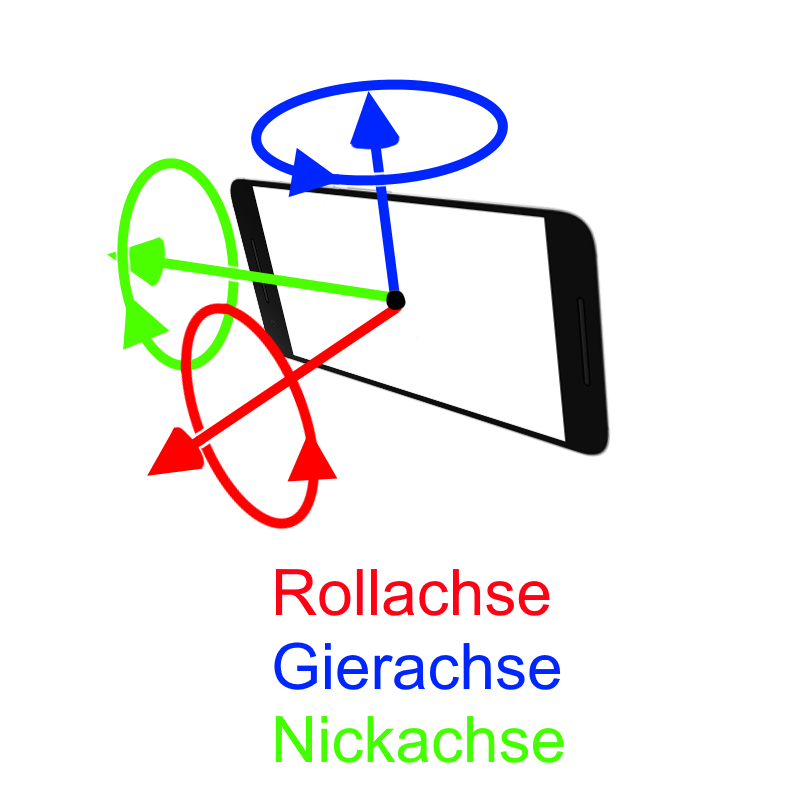
\includegraphics[width=0.5\linewidth]{Reviewdokument/Grafiken/drehachsen.png}
\end{figure}}}

\newglossaryentry{Detektion}{name={Detektion}, description={~\\Lokalisierung eines Merkmals (insb. eines Verkehrszeichens) in einem Bild}}

\newglossaryentry{Fahrzeug}{name={Fahrzeug}, description={~\\Handelsüblicher Personenkraftwagen (PKW), insbesondere kein Lastkraftwagen\\ (LKW)}}

\newglossaryentry{Filter}{name={Filter}, description={~\\Ein Verarbeitungsschritt. Jeder Filter hat eine Dateneingabe und eine -ausgabe. In jedem Verarbeitungsschritt werden die einkommenden Daten umgewandelt. Bei der Umwandlung können den Daten Teile entnommen, hinzugefügt oder auch vollständig ersetzt werden. Die Art der Umwandlung wird durch den Filter bestimmt}}

\newglossaryentry{Filterverwaltungs-Bibliothek}{name={Filterverwaltungs-Bibliothek}, description={~\\Programm-Bibliothek, welche Möglichkeiten bietet, Filter und Neuronale Filter zu laden und auf Bildserien anzuwenden}}

\newglossaryentry{FLOPs}{name={FLOPs}, 
description={Floating Point Operations.\\Operationen auf Fließkommazahlen, die von der \gls{ALU} ausgeführt werden. Sie gelten als eine der aufwendigsten, elementaren Operationen und bestimmen maßgeblich die Laufzeit eines Programms. Ausdrücklich zu unterscheiden von \glqq FLOPS\grqq}}

\newglossaryentry{FLOPS}{name={FLOPS}, 
description={Floating Point Operations per Second.\\Maß für die Leistungsfähigkeit von Computern. Ausdrücklich zu unterscheiden von \glqq FLOPs\grqq}}

\newglossaryentry{Geschwindigkeitsschild}{name={Geschwindigkeitsschild}, description={~\\Gibt die zulässige Höchstgeschwindigkeit des Fahrzeugs an, an dessen Rückseite es befestigt ist. Siehe §58 \gls{StVZO}}}

\newglossaryentry{GPU}{name={GPU}, 
description={Graphics Processing Unit; Grafikkarte.\\ Rechen- und Steuerwerk einer Rechenmaschine, hier insb. eines Personalcomputers oder eines Smartphones, welches auf die Bildverarbeitung spezialisiert ist}}

\newglossaryentry{Keras}{name={Keras}, description={~\\Deep-Learning-Framework in Python basierend auf TensorFlow}}

\newglossaryentry{Klassifikation}{name={Klassifikation}, description={~\\Einteilung eines Merkmals in eine Klasse von Urbildern}}

\newglossaryentry{Konfidenz}{name={Konfidenz}, description={~\\Sicherheit, dass das Objekt korrekt klassifiziert wurde}}

\newglossaryentry{Label}{name={Label}, description={~\\ Meta-Informationen zu einem Sample. In diesem Zusammhang die Position, Größe und Art von Verkehrsschildern in einer Bildaufnahme}}

\newglossaryentry{mAP}{name={mAP}, description={mean Average Precision.\\Maß für die Genauigkeit eines Objekt-Detektors und -Klassifikators. Basiert auf der Position und Größe des vermuteten Bildausschnitts sowie der Rangverteilung der vermuteten Klasse}}

\newglossaryentry{Multithreading}{name={Multithreading}, description={Nebenläufigkeit.\\ Gleichzeitiges Abarbeiten mehrerer Threads innerhalb eines Prozesses}}

\newglossaryentry{Neuronaler Filter}{name={Neuronale Filter}, description={~\\Ein Filter, dessen Umwandlungsvorgehen durch ein Neuronales Netz bestimmt wird}}

\newglossaryentry{Neuronales Netzwerk}{name={Neuronales Netzwerk}, description={~\\Hier im Besonderen: Künstliches Neuronales Netzwerk. Simplifiziertes Modell eines Nervensystems, bestehend aus künstlichen Neuronen, welche auf Computern trainiert werden, um komplexe Aufgaben im Bereich der künstlichen Intelligenz zu bewältigen}}

\newglossaryentry{Nutzer}{name={Nutzer}, description={~\\Der aktuelle Fahrzeugführer, während sich das Fahrzeug nicht in Fahrt befindet bzw. der Beifahrer, während sich das Fahrzeug in Fahrt befindet. Es wird das generische Maskulinum verwendet}}

\newglossaryentry{OpenCV2}{name={OpenCV2}, description={Open Source Computer Vision Library. \\Quelloffene Computergrafikbibliothek. Hier verwendet um Datensätze sowie das erfasste Kamerabild auf die Eingabespezifikationen der Neuronalen Netzwerke anzupassen}}

\newglossaryentry{Produkt}{name={Produkt}, description={~\\Die Kombination aus App und API, welche im Rahmen dieses Softwareprojektes entwickelt werden}}

\newglossaryentry{Pipe}{name={Pipe}, description={~\\Eine Pipe stellt eine Verbindung zwischen den einzelnen Verarbeitungsschritten dar}}

\newglossaryentry{Pipes and Filters}{name={Pipes and Filters}, description={auch Datenfluss-System.\\ Ein Architekturmuster welches die Struktur für Systeme, die Datenströme verarbeiten, darstellt}}

\newglossaryentry{Protobuf}{name={Protocol Buffers, Protobuf}, description={~\\Bezeichnet ein von Google entwickeltes, programmiersprachen- und plattformunabhängiges Format sowie die dazugehörige Implementierung für die Serialisierung und Deserialisierung strukturierter Daten.}}

\newglossaryentry{Sample}{name={Sample}, description={~\\In diesem Zusammenhang eine Bildaufnahme von Verkehrszeichen, welche Neuronalen Netzwerken präsentiert werden können, um sie zur Detektion und Klassifkation zu trainieren}}

\newglossaryentry{Smartphone}{name={Smartphone}, description={~\\Mobiles Endgerät, welches über eine integrierte Kamera verfügt und den im Pflichtenheft spezifizierten Bedingungen genügt}}

\newglossaryentry{SoC}{name={SoC}, description={System-on-a-Chip.\\ Kombination von CPU, Bus, Taktgeber, Co-CPUs, GPU, Soundchip, Interfaces, etc. oder Teilen davon auf einem Chip. Häufig verwendet in mobilen Endgeräten und eingebetteten Systemen um durch hohe Integrationsdichten Fläche auf der Platine einzusparen}}

\newglossaryentry{StVO}{name={StVO}, description={Straßenverkehrsordnung\footlink{https://www.gesetze-im-internet.de/stvo\_2013/StVO.pdf}{29.04.2018}}}

\newglossaryentry{StVZO}{name={StVZO}, description={Straßenverkehrszulassungsordnung\footlink{https://www.gesetze-im-internet.de/stvzo\_2012/StVZO.pdf}{29.04.2018}}}

\newglossaryentry{System}{name={System}, description={~\\Gesamtheit aus Halterung, Smartphone und App}}

\newglossaryentry{Tracking}{name={Tracking}, description={~\\Objekte anhand primitiver Merkmale in einer Bildserie oder einem Video lokalisieren und verfolgen}}

\newglossaryentry{TensorFlow Lite}{name={TensorFlow Lite}, description={~\\Für mobile Endgeräte optimiertes Deep-Learning-Framework des Google Brain Teams\footlink{https://www.tensorflow.org/mobile/tflite/}{29.04.2018}}}

\newglossaryentry{TensorFlow Mobile}{name={TensorFlow Mobile}, description={~\\Deep-Learning-Framework des Google Brain Teams, welches zwar für Android noch keine GPU Unterstützung bietet, dafür aber derzeit noch bzgl. der Kompatibilität besser von bereits etablierten Netzwerken unterstützt wird}}

\newglossaryentry{Tensorflow Node}{name={Tensorflow Node},description={~\\Ein Knoten (Node) im Sinne von TensorFlow bezeichnet eine bestimmte Operation innerhalb des Netzwerk Models: Es ist die grundlegende Einheit für Berechnungen innerhalb von TensorFlow. Die Ergebnisse dieser Knoten lassen sich anhand deren Bezeichnungen (zum Beispiel \glqq{}final\_output\qrqq{})  einzeln abfragen}}

\newglossaryentry{UI}{name={UI},description={User Interface.\\ Benutzeroberfläche}}

\newglossaryentry{VZ}{name={VZ}, description={Verkehrszeichen}}

\newglossaryentry{Verkehrszeichen-API}{name={Verkehrszeichen-API}, description={~\\Besondere Programmierschnittstelle, die für Verkehrszeichenerkennung optimiert ist und erweiterte Logik zur Verfügung stellt, wie etwa die Abschätzung, wann ein Verkehrsschild passiert wurde und damit gültig ist und angezeigt werden muss}}

\newglossaryentry{Verkehrszeichenkombination}{name={Verkehrszeichenkombination}, description={~\\Gruppe von untereinander angebrachten Verkehrszeichen, welche einen gemeinsamen Sinnzusammenhang darstellen}}

\newglossaryentry{VwV-StVO}{name={VwV-StVO}, description={Allgemeine Verwaltungsvorschrift
zur Straßenverkehrs-Ordnung\footlink{http://www.verwaltungsvorschriften-im-internet.de/bsvwvbund\_26012001\_S3236420014.htm}{29.04.2018}}}



\author{
    [Projektgruppe 2]\\~\\
    \textit{Namen entfernt}\\~\\
    \textcolor{red}{Verwendung nur zu Lehrzwecken an der TU Ilmenau. Die Verwendung}\\\textcolor{red}{für private oder kommerzielle Zwecke ohne Einwilligung der Autoren ist}\\ \textcolor{red}{ausdrücklich untersagt.}\\~\\
    Kontakt: \href{mailto:signapse.app@gmail.com}{signapse.app@gmail.com}
    %Bock, Robert Niklas\\ \texttt{robert-niklas.bock@tu-ilmenau.de}\\~\\
    %Dirbas, Mohammad\\ \texttt{mohammad.dirbas@tu-ilmenau.de} \\~\\
    %Fischedick, Söhnke Benedikt\\ \texttt{soehnke-benedikt.fischedick@tu-ilmenau.de} \\~\\
    %Hampel, Jakob Frank\\ \texttt{jakob.hampel@tu-ilmenau.de} \\~\\
    %Köhler, Florian\\ \texttt{florian.koehler@tu-ilmenau.de} \\~\\
    %Langer, Patrick\\ \texttt{patrick.langer@tu-ilmenau.de} \\~\\
    %Nowati, Yusuf\\ \texttt{yusuf.nowati@tu-ilmenau.de} \\~\\
    %Treichel, Tim\\ \texttt{tim.treichel@tu-ilmenau.de} \\ ~\\ ~\\ ~\\ ~\\
}

\title{Abschluss-Reviewdokument\\Verkehrszeichenerkennung}
\begin{document}
\maketitle
\renewcommand{\arraystretch}{1.5}
\tableofcontents

% -----------------------------------------

\part{Bisheriger Projektablauf}

\chapter{Einleitung}

\section{Ausganssituation}
Die meisten Autofahrer kennen das Gefühl der Unsicherheit über die aktuell erlaubte Höchstgeschwindigkeit. Daher verfügen viele moderne Fahrzeuge über eine automatische Verkehrszeichenerkennung, mit deren Hilfe der Fahrzeugführer zu jedem Zeitpunkt über die aktuell geltenden Verkehrsregelungen informiert ist. Der Fahrzeugführer kann beispielsweise stets die zulässige Geschwindigkeit nachvollziehen und gegebenenfalls auf ein Überschreiten dieser hingewiesen werden. Die Verkehrszeichenerkennung ist dabei meist als Fahrerassistenzsystem fest im \gls{Fahrzeug} verankert und nutzt zur Erkennung der Verkehrszeichen eine in Höhe des Innenspiegels angebrachte Kamera. Folglich ist ein solches Assistenzsystem ausschließlich modernen Fahrzeugen mit entsprechender Ausstattung vorbehalten und mit einem hohen Aufpreis verbunden.\\

Bisher existierte keine, mit diesem Projekt vergleichbare, praktikable Möglichkeit, ein solches Assistenzsystem auch in älteren und preisgünstigeren Fahrzeugen nachzurüsten. Zwar sind diverse Apps zur Verkehrszeichenerkennung für Android und iOS bereits verfügbar, allerdings ist keine davon in der Lage, mit der in diesem Projekt geplanten Verlässlichkeit und Performanz geschwindigkeitsregulierende Verkehrszeichen und \glslink{Verkehrszeichenkombination}{Verkehrszeichenkombinationen} zu erkennen.\\


\section{Ziel}
Ziel dieses Softwareprojektes ist es, ein \gls{System} (bestehend aus einem \gls{Smartphone}, einer KFZ-Smartphonehalterung und einer \gls{App}) zur Verkehrszeichenerkennung zu entwickeln,
welches in jedem \gls{Fahrzeug} nachgerüstet werden kann. Inhalt der dafür zu entwickelnden \gls{App} ist eine Benutzerschnittstelle, welche erkannte Verkehrszeichen während der Fahrt anzeigt, sowie eine Logik-Schnittstelle (als \gls{API}), welche in Echtzeit aus Kameraaufnahmen Verkehrsschilder identifiziert, aber derart modular aufgebaut ist, um auch andere \gls{Detektion}s- und \gls{Klassifikation}sprobleme zu lösen.\\

\section{Produktbeschreibung}
Das Produkt besteht aus einer Android-\gls{App} sowie einer wiederverwendbaren \gls{API}, im Folgenden \gls{Filterverwaltungs-Bibliothek} genannt. Um die \gls{App} an diese \gls{Filterverwaltungs-Bibliothek} anzubinden, existiert ferner die sogenannte \gls{Verkehrszeichen-API}, welche die \gls{Filterverwaltungs-Bibliothek} für das konkrete Problem der Verkehrszeichenerkennung konfiguriert und in die \gls{App} eingebunden ist.\\
Das \gls{System} soll von Fahrzeugführern mit Android-Smartphone bzw. deren Beifahrer verwendet werden. Hauptfunktion des \glslink{System}{Systemes} ist die Erkennung der in \cref{sec:liste_zu_erkennende_verkehrszeichen} spezifizierten Verkehrszeichen.\\

\subsection{Produktmerkmale}

\begin{itemize}

\item Die Verkehrszeichenerkennung funktioniert bei klarer Sicht und Tageslicht bis zu einer maximalen Geschwindigkeit von 150 km/h.

\item Das \gls{System} kann unter genauer Spezifikation von Halterung und Spannungsversorgung für das \gls{Smartphone} in jedem \gls{Fahrzeug} nachgerüstet werden.

\item Der \gls{Nutzer} wird zur richtigen Ausrichtung des \glslink{Smartphone}{Smartphones} bei Stillstand des Fahrzeugs mit einer Kalibrierungsphase unterstützt. Er erhält dazu Anweisungen auf dem Bildschirm.

\item Die Erkennung von Verkehrszeichen, Zusatz- und Sonderschildern durch die \gls{App} ist auf solche beschränkt, welche einen Einfluss auf die zulässige Höchstgeschwindigkeit sowie den Geltungsbereich derselben haben.

\item Die \gls{App} ist in der Lage, \glslink{Geschwindigkeitsschild}{Geschwindigkeitsschilder} (gemäß §58 \gls{StVZO}) auf LKWs herauszufiltern, um ein fehlerhaftes Anzeigen zu vermeiden.

\item Die Erkennung der Verkehrszeichen erfolgt in Echtzeit, das heißt videotaktschritthaltend. Nach dem Passieren eines Verkehrszeichens entsteht höchstens eine Verzögerung von 1 s bis zum Erscheinen des Verkehrszeichens auf dem Display.

\item Die Kernfunktionalität zur \gls{Detektion} und \gls{Klassifikation} von Verkehrszeichen im Kamerabild ist auf andere \glslink{Detektion}{Detektionsprobleme} übertragbar. Dafür wurde dieser Aspekt in die bereits genannte \glqq{}\gls{Filterverwaltungs-Bibliothek}\grqq{} ausgelagert.

\item Die aktuelle Geschwindigkeit kann nach Wunsch des \gls{Nutzer}s mittels GPS erfasst werden. Bei Überschreitung der zulässigen Geschwindigkeit - ermittelt aus dem aktuell erkannten Verkehrszeichen - wird eine entsprechende Warnung auf dem Display dargestellt.

\item Die Benutzeroberfläche steht sowohl in deutscher als auch englischer Sprache zur Verfügung.

\item Die Erkennung ist mittels \glslink{Neuronales Netzwerk}{Neuronaler Netzwerke} realisiert.

\item Die \gls{App} ist ohne aktive Internetverbindung nutzbar. Es wird lediglich das GPS benötigt.

\end{itemize}

Damit das \gls{System} diese Funktionalitäten auch jederzeit korrekt erfüllen kann, muss eine Reihe von Betriebsbedingungen erfüllt sein.\\

\subsection{Betriebsbedingungen}
\begin{itemize}

\item Die Verkehrszeichenerkennung der \gls{App} ist für Geschwindigkeiten bis zu 150km/h ausgelegt.

\item Das \gls{Smartphone}, auf welchem die \gls{App} ausgeführt wird, muss an der Windschutzscheibe bzw. in der Nähe der Windschutzscheibe auf dem Armaturenbrett des Fahrzeugs montiert werden. Die Kamera muss ein freies Sichtfeld auf den Verkehr besitzen und in einem von der \gls{App} festgelegten Winkel auf die Fahrbahn zeigen. Damit dies erreicht werden kann, gibt es eine Anleitung zur Ausrichtung in der \gls{App}.

\item Die zu erkennenden Verkehrszeichen müssen gemäß \gls{VwV-StVO} §§ 39-43 aufgestellt sein und sich im Originalzustand befinden.

\item Die Verkehrszeichenerkennung wird nur bei Tag und bei klarer Sicht (kein Nebel, kein Niederschlag, kein starkes Gegenlicht) garantiert. (Unter diesen Umständen und einem dunklen Armaturenbrett stellen Spiegelungen an der Frontscheibe kein Problem dar.)

\item Um eine dauerhafte Nutzung zu gewährleisten, muss das \gls{Smartphone} mit einem ausreichend starken Ladegerät verbunden sein. Der verwendete USB-Port sollte erfahrungsgemäß mindestens 2 A bei 5 V liefern. Die meisten in Autos integrierten USB-Anschlüsse liefern allerdings nicht diese Leistung. Deshalb sollte stattdessen ein KFZ-Ladeadapter mit entsprechend beschriebenen Leistungsfähigkeiten verwendet werden. Das Ladekabel muss zudem in der Lage sein, die beschriebene Leistung zu übertragen. Es ist deshalb empfehlenswert, das Original-Ladekabel oder ein entsprechend der Leistung ausreichend spezifiziertes Kabel zu verwenden. Ein guter Indikator für nicht ausreichende Ladeleistung ist ein abnehmender Ladestand trotz angeschlossenem Ladegerät.

\item Der Stromverbrauch des \glslink{Smartphone}{Smartphones} kann verringert werden, indem beispielsweise das Display maximal bei halber Helligkeit gehalten, im Hintergrund laufende Apps wie z.B. Musikwiedergabe beendet oder Funkverbindungen wie WLAN, Bluetooth oder NFC deaktiviert werden. Bei Bedarf kann die Helligkeit weiter reduziert oder ein anderes Ladegerät und/oder Kabel mit besseren Ladeeigenschaften genutzt werden.

\end{itemize}

\chapter{Entwurf}
Im Sinne des Hauptzieles des Softwareprojektes - die Nachrüstbarkeit auf ältere und preis\-günstigere Fahrzeuge - spielt es eine tragende Rolle, die Funktionalität der Verkehrszeichenerkennung auch auf andere Systeme übertragen zu können. Die \gls{App} wird zwar nur für Android programmiert, aber es soll problemlos möglich sein, mit derselben \gls{API} auch eine \gls{App} für Endgeräte mit anderen Betriebssystemen zu programmieren.\\
Um die gewünschte Portierbarkeit gewährleisten zu können, ist es absolut essentiell, dass die einzelnen Funktionalitäten möglichst modular gestaltet sind. Dies wird mithilfe der im Folgenden absteigend erklärten Abstraktionsebenen umgesetzt.

\begin{description}
\item[App] Die \gls{App} abstrahiert die \gls{Verkehrszeichen-API} dem \gls{Nutzer} gegenüber. Der \gls{Nutzer} weiß unter Umständen überhaupt nicht von der Existenz der \gls{Verkehrszeichen-API}, während er die \gls{App} benutzt, dies stellt für ihn allerdings kein Problem dar. Er soll in der Lage sein, die \gls{App} ohne jedwedes Wissen über die zugrundeliegenden Schnittstellen zu nutzen.

\item[Verkehrszeichen-API] Die \gls{Verkehrszeichen-API} abstrahiert die \glslink{Filterverwaltungs-Bibliothek}{Filterverwaltungs}-Bib\-liothek der \gls{App} gegenüber. Die \gls{App} greift auf die \gls{Verkehrszeichen-API} zu und sieht diese lediglich als Black Box. Dies ist insoweit wichtig, als dass für die eventuelle Realisierung einer iOS-\gls{App} exakt dieselbe Funktionalität gewährleistet werden kann.\\
Die \gls{Verkehrszeichen-API} kann also wiederverwendet werden, um dieses konkrete Problem der Verkehrszeicherkennung auf beliebigen Endgeräten realisieren zu können.

\item[Filterverwaltungs-Bibliothek] Die \gls{Filterverwaltungs-Bibliothek} abstrahiert die ihr zugrundeliegende \glslink{Pipes and Filters}{Pipes-and-Filters-Architektur} der \gls{Verkehrszeichen-API} gegenüber. Mit ihr soll es möglich sein, nach Belieben Filter zu implementieren, die den Datenstrom weiterverarbeiten. In diesem Falle kann ein Filter beispielsweise eine Entzerrung durchführen, ein Input-Bild zuschneiden - oder eben ein \gls{Neuronales Netzwerk} darauf anwenden.\\
Die \gls{Filterverwaltungs-Bibliothek} kann dementsprechend wiederverwendet werden, um beliebige \glslink{Detektion}{Detektions-} und \gls{Klassifikation}sprobleme auf verschiedenen Endgeräten (die Tensorflow unterstützen) umzusetzen.

\end{description}

\section{Systemzerlegung}

\begin{figure}[H]
\centering
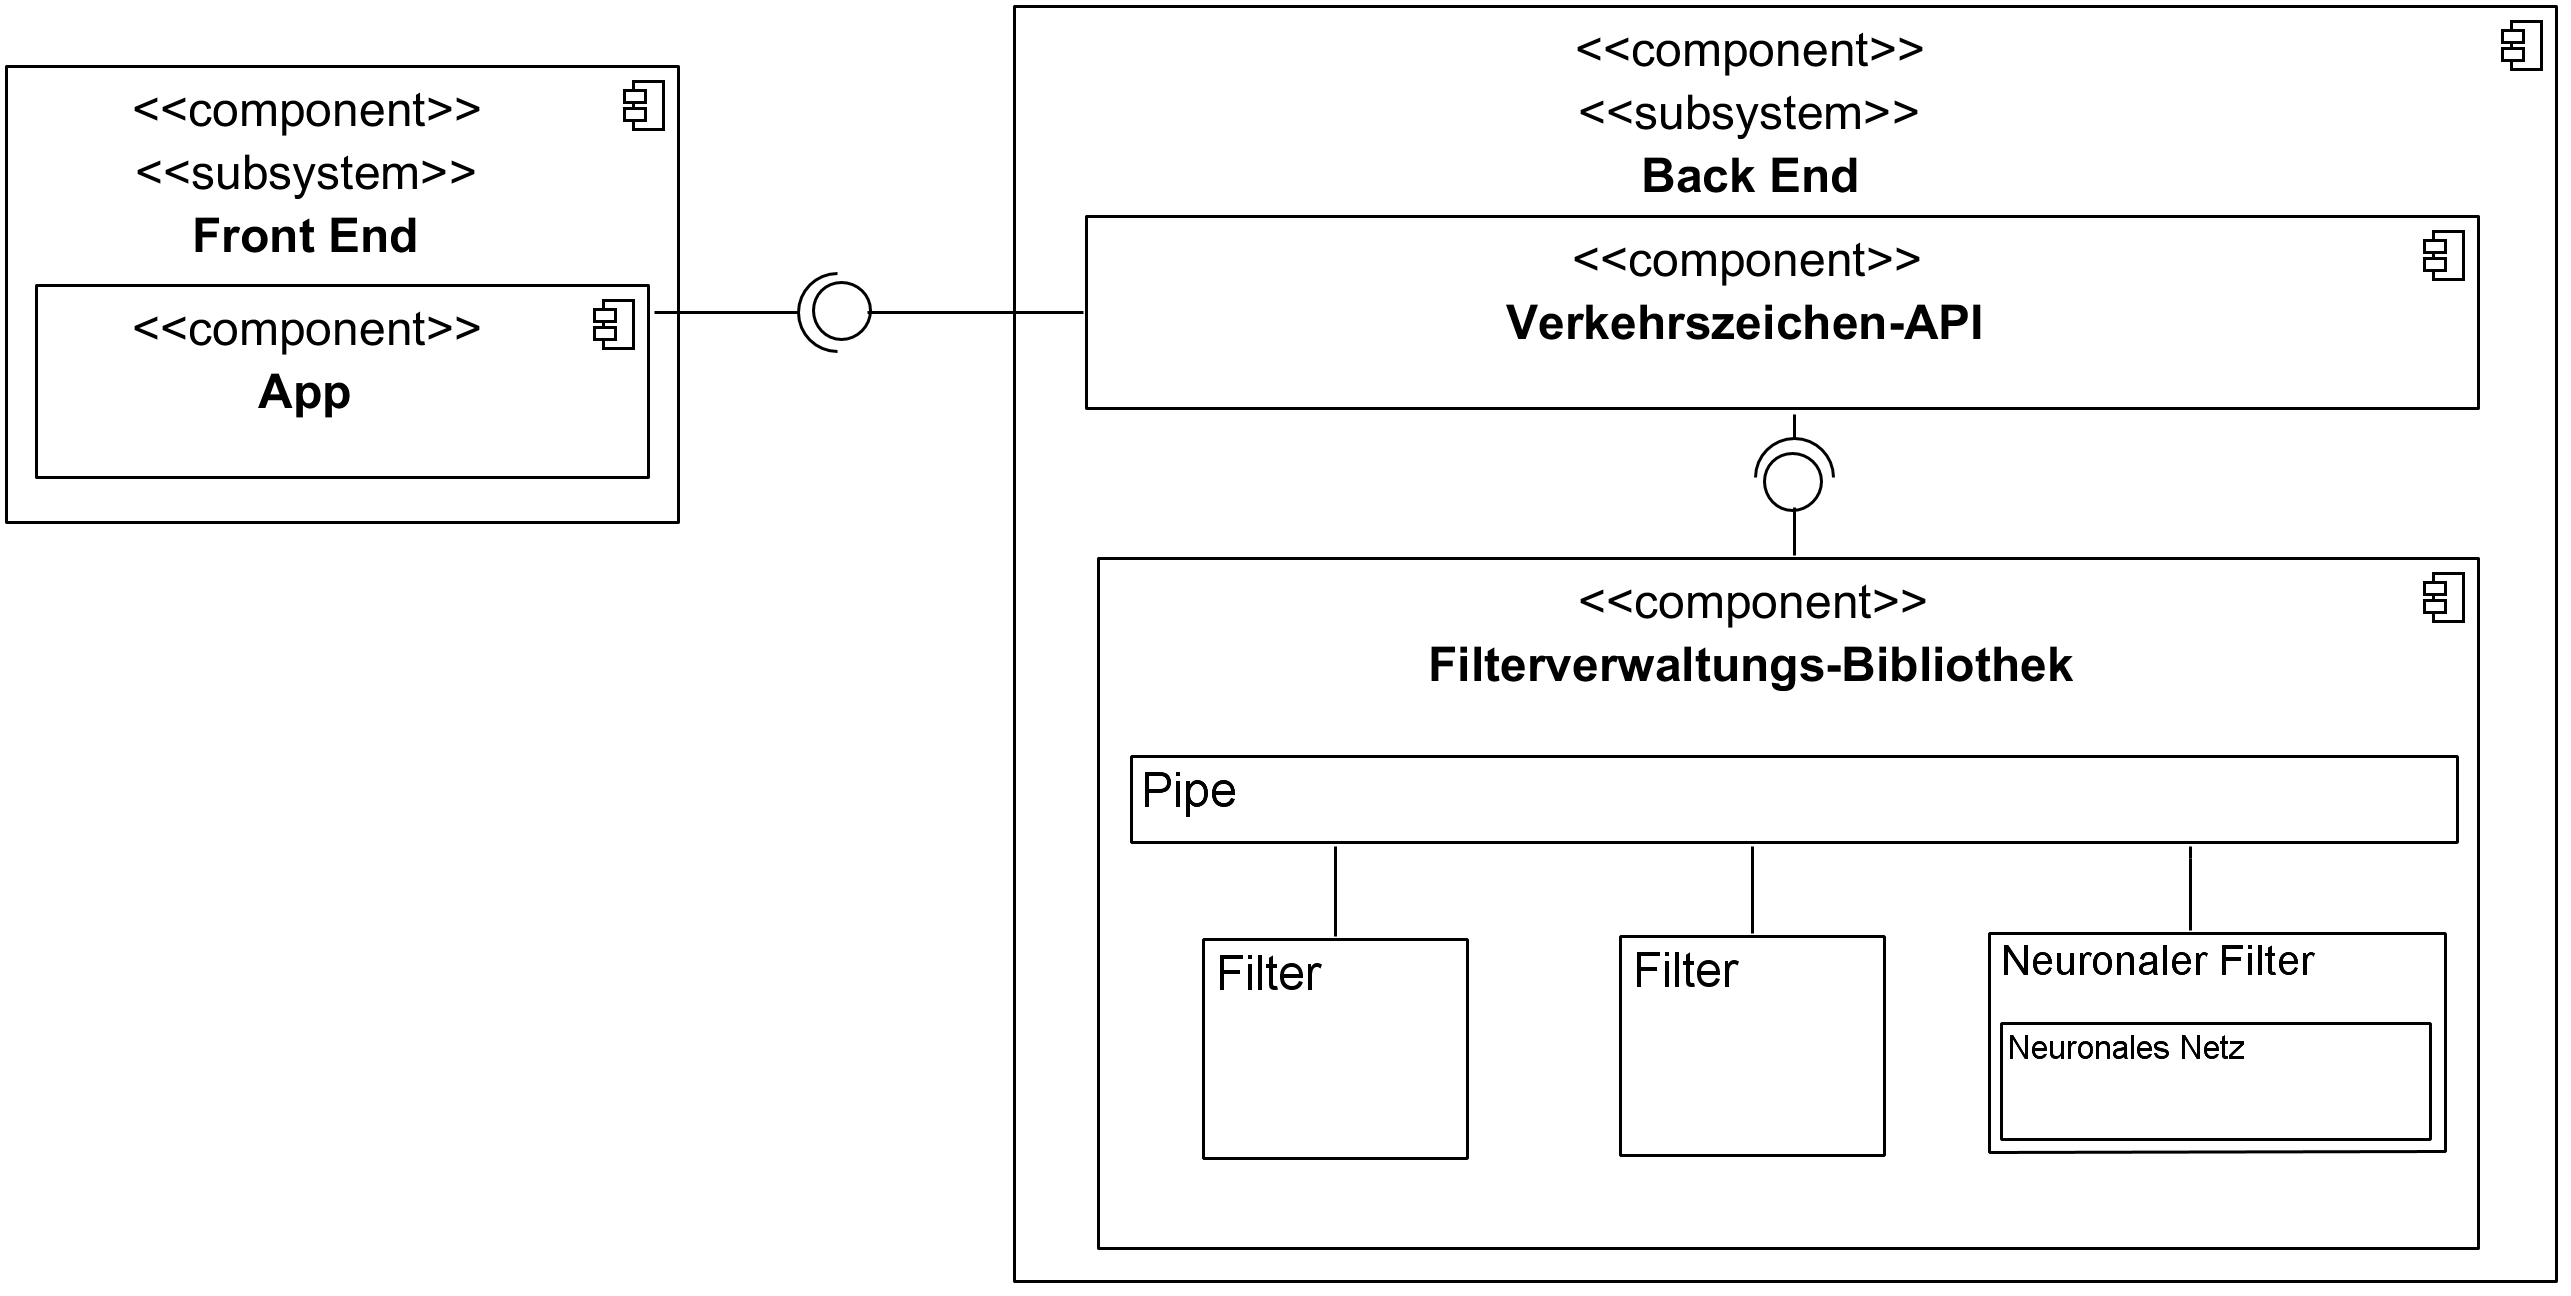
\includegraphics[width=1\linewidth]{Grafiken/component_diagram_neu.png}
\caption{Subsystemstruktur}
\end{figure}
\label{sec:subsystemstruktur}

Die Funktionalität der Verkehrszeichenerkennung wird aus der \gls{App} ausgelagert. Das Ziel ist dabei, diese Funktionalität möglichst modular zu gestalten, damit sie auf verschiedenen Endgeräten mit verschiedenen Betriebssystemen zum Einsatz kommen kann, während die \gls{App} vorerst ausschließlich für Android vorgesehen ist. Dabei wird das \gls{System} in zwei Subsysteme zerlegt - Front End und Back End. Das Front End wird von der \gls{App} realisiert und stellt lediglich die Benutzeroberfläche sowie einige Kleinigkeiten (z.B. die Geschwindigkeitsanzeige) zur Verfügung. Das Back End besteht aus der \gls{Verkehrszeichen-API}, welche ihrerseits auf die  \gls{Filterverwaltungs-Bibliothek}  zugreift.\\
Die \gls{App} greift, wenn sie ein Verkehrszeichen erkennen soll, auf die \gls{Verkehrszeichen-API} zu, welche die einzige Schnittstelle der \gls{App} zu den \gls{Detektion}s- und \gls{Klassifikation}snetzwerken darstellt. Dabei werden die beiden \glslink{Neuronales Netzwerk}{Neuronalen Netzwerke} als \gls{Filter} in der \gls{Filterverwaltungs-Bibliothek} realisiert. Ferner existiert ein  \gls{Filter}, welches die Aufgabe hat, den detektiereten Bildauschnitt zuzuschneiden, sodass das \glslink{Klassifikation}{Klassifikationsfilter} darauf arbeiten kann.\\
Das Ziel dieses gewählten Entwurfes ist es, die Schnittstelle zwischen \gls{App} und \gls{API}s möglichst einfach zu halten und das gesamte zugrundeliegende Netzwerk soweit wie möglich zu abstrahieren. Aus Sicht der \gls{App} existiert keine \gls{Filterverwaltungs-Bibliothek}. Die \gls{App} \glqq{}sieht\grqq{} nur die \gls{Verkehrszeichen-API} als Black Box.\\

\section{Zugrundeliegende Architektur}

\subsection{App}
Die \gls{App} ist aus einzelnen Komponenten aufgebaut, im Android-Jargon auch als \textit{Fragmente}\footnote{\link{https://developer.android.com/guide/components/fragments}, 15.06.2018} bezeichnet werden. Zu jedem Fragment gehört ein \gls{UI} sowie mindestens eine Java-Klasse, wodurch die zugehörige Funktionalität realisiert wird. Im Allgemeinen können mehrere Fragmente gleichzeitig aktiv sein, aber für dieses Projekt wurde sich dafür entschieden, nur höchstens ein aktives Fragment gleichzeitig zuzulassen. Der Grund liegt darin, dass die in einzelne Fragmente ausgelagerten Funktionalitäten in der Anwendung später disjunkt sind; so kann das \gls{System} beispielsweise nicht gleichzeitig kalibriert und verwendet werden. Die Entscheidung für die Verwendung solcher Fragmente liegt in ihrer Kapselung begründet, sowie in dem Vorteil ihrer einfachen Handhabung und der daraus erwachsenden einfachen Erweiterbarkeit der Anwendung.\\

\subsection{API}
Die \gls{Filterverwaltungs-Bibliothek} ist nach dem \glslink{Pipes and Filters}{Pipes-and-Filters}-Prinzip aufgebaut. Dieses ist ein gängiges Architekturmuster für \glslink{System}{Systeme}, die Datenströme verarbeiten. In unserem Fall bestehen diese aus (einer Folge von) Einzelbildern mit einem Header, in dem Zusatzinformationen Platz finden.\\
Ein \gls{Filter} stellt dabei einen Verarbeitungsschritt dar, wobei jeder \gls{Filter} der \gls{Pipe} ein Bild entgegennimmt und auch wieder ein Bild herausgibt. Darüber hinaus kann jeder \gls{Filter} dem Datenpaket bestimmte Metainformationen beifügen, die später für eine genauere Analyse verwendet werden können. Wenn beispielsweise ein \gls{Filter} ein Verkehrszeichen auf einem Bild an einer bestimmten Position detektiert und im darauffolgenden \gls{Filter} das Verkehrszeichen klassifiziert wird, wird neben dem Zuschneiden des Bildes auf das erkannte Verkehrszeichen auch die Position des Verkehrszeichens im Original als Metainformation gespeichert. Dies ist eine Abwandlung der herkömmlichen \glslink{Pipes and Filters}{Pipes-and-Filters}-Architektur.
Weiterhin ist es möglich, dass sich die \glslink{Pipe}{Pipeline} nach bestimmten Verarbeitungsschritten in mehrere untergeordnete \glslink{Pipe}{Pipes} aufteilt: Werden auf einem Bild mehrere Verkehrszeichen erkannt, wird der \gls{Filter} für die \gls{Klassifikation}  für alle Kandidaten aufgerufen (ggf. parallel). Dies erweitert die originale Architektur zum “Tee-and-Joins-\glslink{Pipes and Filters}{Pipes-and-Filters}-Pipeline-System”.
Die Wahl dieses Architekturmusters ist wie folgt begründet:

\subsubsection{Effizienz}
Alle \gls{Filter} einer \gls{Pipe} arbeiten auf ein- und demselben Datenobjekt im Speicher. Das heißt, dass jeder \gls{Filter} dieses Objekt per Adresse direkt anspricht, ohne es zu  kopieren. 

\subsubsection{Modularität}
Einzelne \gls{Filter} lassen sich individuell austauschen, erweitern oder entfernen. So lassen sich in unserem Fall z.B. einfach \gls{Filter} für verschiedene \glslink{Detektion}{Detektionsstrategien} oder optische Bildaufbereitung einfügen.

\subsubsection{Performanz}
Die Verwendung des \glqq{}Tee-and-Joins-\glslink{Pipes and Filters}{Pipes-and-Filters}-\glslink{Pipe}{Pipeline}-Systems\grqq{} erlaubt es, verschiedene Filteroperationen durch Verwendung mehrerer Threads echt-parallel zu bearbeiten und so Rechenzeit einzusparen.\\

\subsection{Neuronale Netzwerke}
Bereits von vornherein war bekannt, dass offensichtlich ein Trade-Off zwischen Erkennungsqualität und -geschwindigkeit eingegangen werden muss. Der Fokus lag in diesem Falle eindeutig bei der Geschwindigkeit, da es in der Anwendung absolut kritisch ist, die Verkehrszeichen rechtzeitig zu \glslink{Detektion}{detektieren} und zu \glslink{Klassifikation}{klassifizieren}. Zwischen dem Passieren des Verkehrszeichens und der Ausgabe in der \gls{App} darf den Anforderungen gemäß nur höchstens 1 s vergehen, was für die Verwendung \glslink{Neuronales Netzwerk}{Neuronaler Netzwerke} auf Mobilgeräten sehr wenig ist.\\
Die Wahl des Frameworks fiel zunächst auf \gls{TensorFlow Lite}, was auch zu dem Punkt eine kluge Entscheidung war. Etwa in der Mitte der Phase II musste diese Entscheidung allerdings revidiert werden. Der Grund dabei lag darin, dass sich nach Tests verschiedener \glslink{Detektion}{Detektoren} SSDLite\cite{DBLP:journals/corr/abs-1801-04381} als sinnvollste Architektur herausstellte, was aber nicht mit \gls{TensorFlow Lite} kompatibel ist - von daher wurde \gls{TensorFlow Mobile} gewählt. Genaueres dazu ist im nachfolgenden Kapitel erläutert.\\

\chapter{Realisierung des Entwurfes}

In diesem Kapitel sei die Umsetzung des Entwurfes in Phase II beschrieben. Änderungen, bzw. Erweiterungen der Implementierung sind im nachfolgenden Teil beschrieben.

\section[Meilenstein 1: App Prototyp]{Meilenstein 1: App Prototyp, bis 02.05 (50 PS)}
Das \gls{UI} des Prototypes in \cref{fig:detektor_ui} wurde zum Ende von Phase I erstellt und wurde seitdem ständig weiterentwickelt.\\

\begin{figure}[H]
\centering
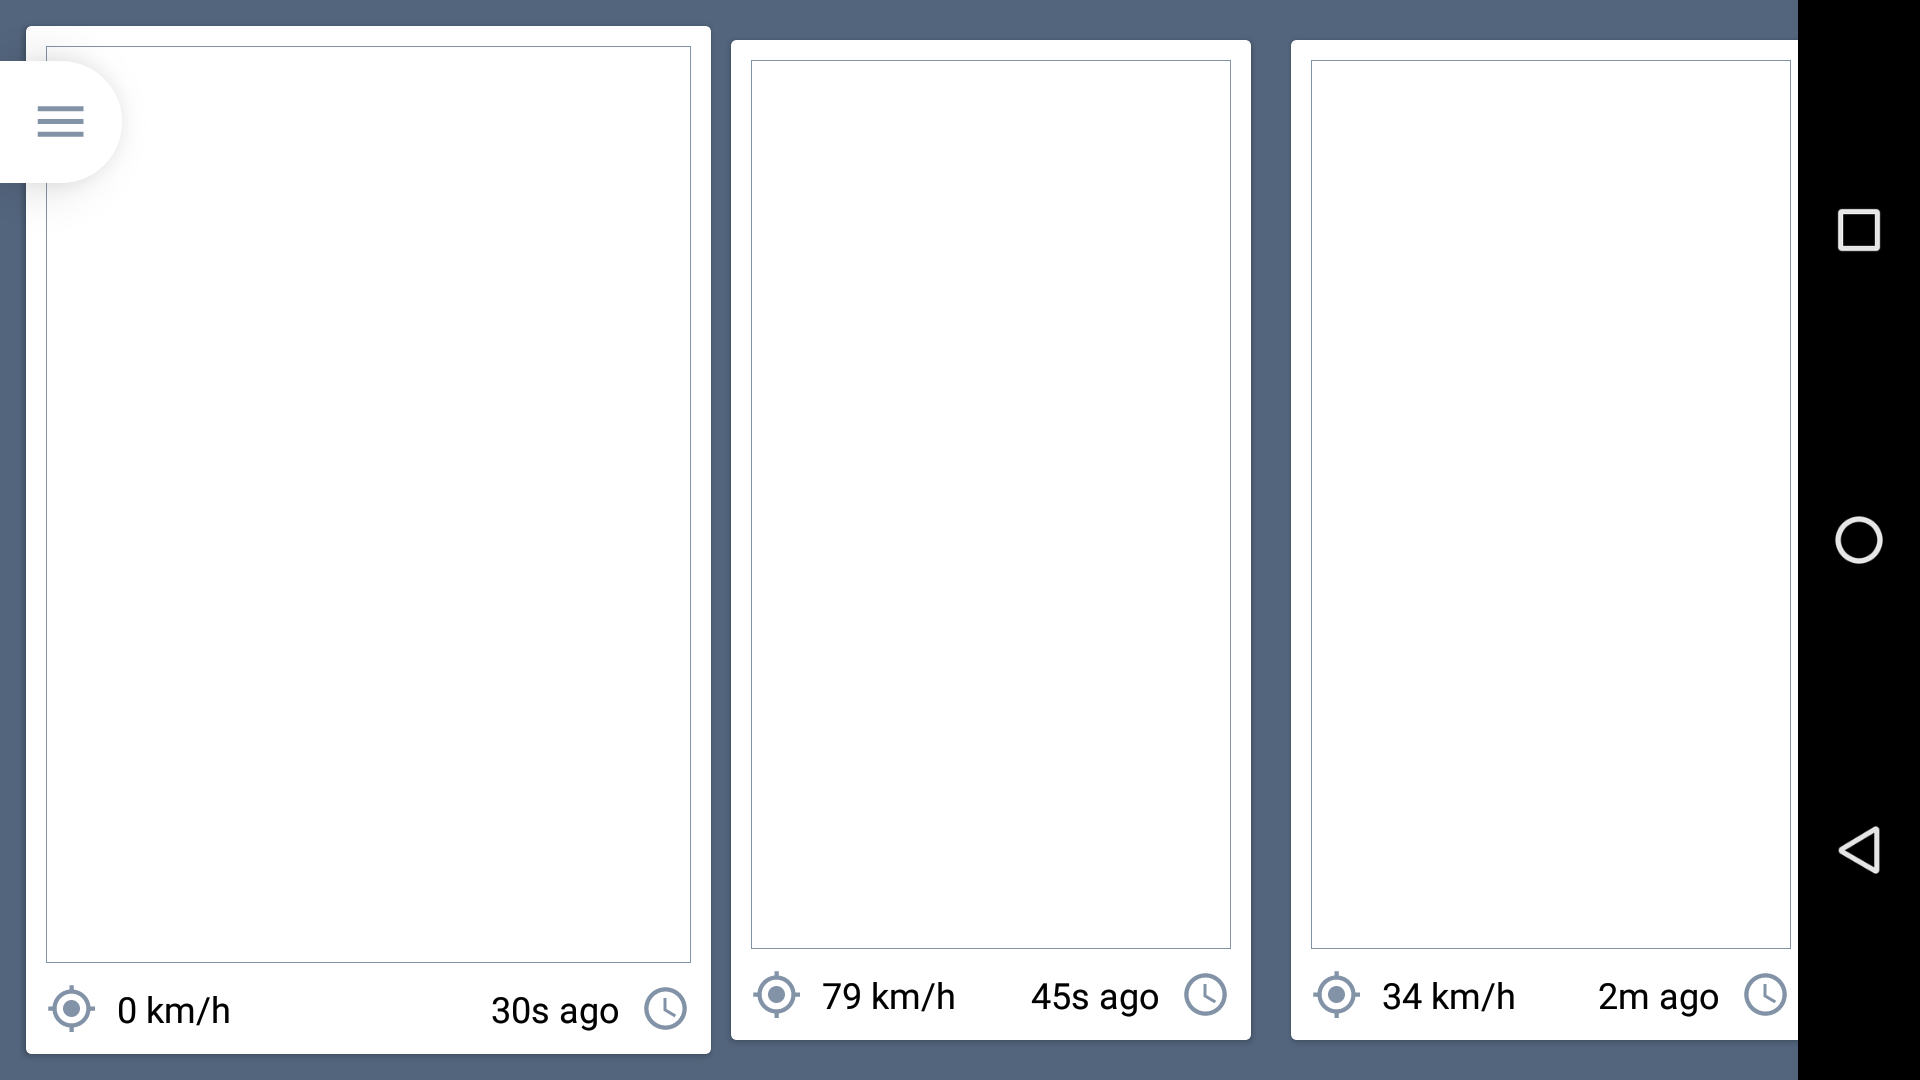
\includegraphics[width=0.9\linewidth]{Reviewdokument/Grafiken/app_detector_screenshot_old.png}
\caption{\gls{UI} des Detektor-Fragmentes zu Ende der ersten Iteration}
\label{fig:detektor_ui}
\end{figure}

\section[Meilenstein 2: Aufnahme und Labeln aller Samples]{Meilenstein 2: Aufnahme und Labeln aller Samples, bis 10.06. (300 PS)}

Die \glslink{Sample}Samples wurden aufgenommen, komplett gelabelt und sortiert. Wie in der Aufwandsabschätzung in Phase II beschrieben, hat dies deutlich länger gedauert als ursprünglich geplant. Neben den in \cref{sec:liste_zu_erkennende_verkehrszeichen} spezifizierten Verkehrszeichen wurden auch einige spezielle Gefahrenzeichen gelabelt. Dies liegt darin begründet, dass diese Gefahrenzeichen einen Einfluss auf die zulässige Höchstgeschwindigkeit haben, wenn sie an dem selben Mast hängen und damit den Geltungsbereich  eines geschwindigkeitsregulierenden Verkehrszeichens einschränken.\\

Ferner wurde es für vorteilhaft erachtet, alle Verkehrszeichen zu labeln, auch wenn diese auf die Geschwindigkeitsbeschränkung keinen Einfluss haben. Der Grund dafür ist, dass einige sehr unüblich gefärbte Verkehrszeichen, bspw. der Vorwegweiser, ggf. später als ähnliche Verkehrszeichen - z.B. die Orstafel  - klassifizieren werden könnten, weil dem \glslink{Neuronales Netzwerk}{Neuronalen Netzwerk} nur die Ortstafel präsentiert wurde und keine Abgrenzung zu den ähnlichen Schildern stattgefunden hat.\\
In \cref{sec:eigens_gelabelte_verkehrszeichen} ist eine Liste der dem ursprünglichen Datensatz (sh. \cref{sec:datensatz}) hinzugefügten Verkehrszeichen zu finden.\\
 
\section[Meilenstein 3: App]{Meilenstein 3: App, bis 10.06. (155 PS)}
Dieser Meilenstein beinhaltet die \gls{App}, allerdings noch ohne Einbindung der \gls{API}. Der Meilenstein 3 ist erreicht, wenn das \gls{UI} vorhanden ist, die Kameraanbindung sowie die Geschwindigkeitsmessung funktioniert und wenn eine Möglichkeit zur Kalibrierung des Gerätes mittels Gravitationssensor oder Gyroskop vorhanden ist. Das \gls{UI} wurde bereits in der letzten Iteration begonnen.\\

Die Kameraanbindung stellte aufgrund der hohen Komplexität der in Android bereitgestellten Camera2-\gls{API}\footnote{\link{https://developer.android.com/reference/android/hardware/camera2/package-summary}, 02.07.2018} ein großes Problem dar, wurde aber termingerecht fertiggestellt und funktioniert wie gefordert (Pflichtenheft P4302).\\
Während der Implementierung wurde temporär ein weiteres, nicht im Feinentwurf aufgelistetes Fragment eingefügt - \texttt{TSDDebugFragment} - welches Informationen über die \gls{Smartphone}-Kamera bereitstellt (sh. \cref{fig:debug_ui}). Beispielsweise werden dort die verschiedenen Kameras, die verschiedenen Autofokus-Modi der jeweiligen Kameras sowie das aktuelle Kamerabild angezeigt. Wie der Name bereits vermuten lässt, dient dieses Fragment ausschließlich zum Debugging und ist \emph{nicht} Teil der fertigen \gls{App}.\\

\begin{figure}[H]
\centering
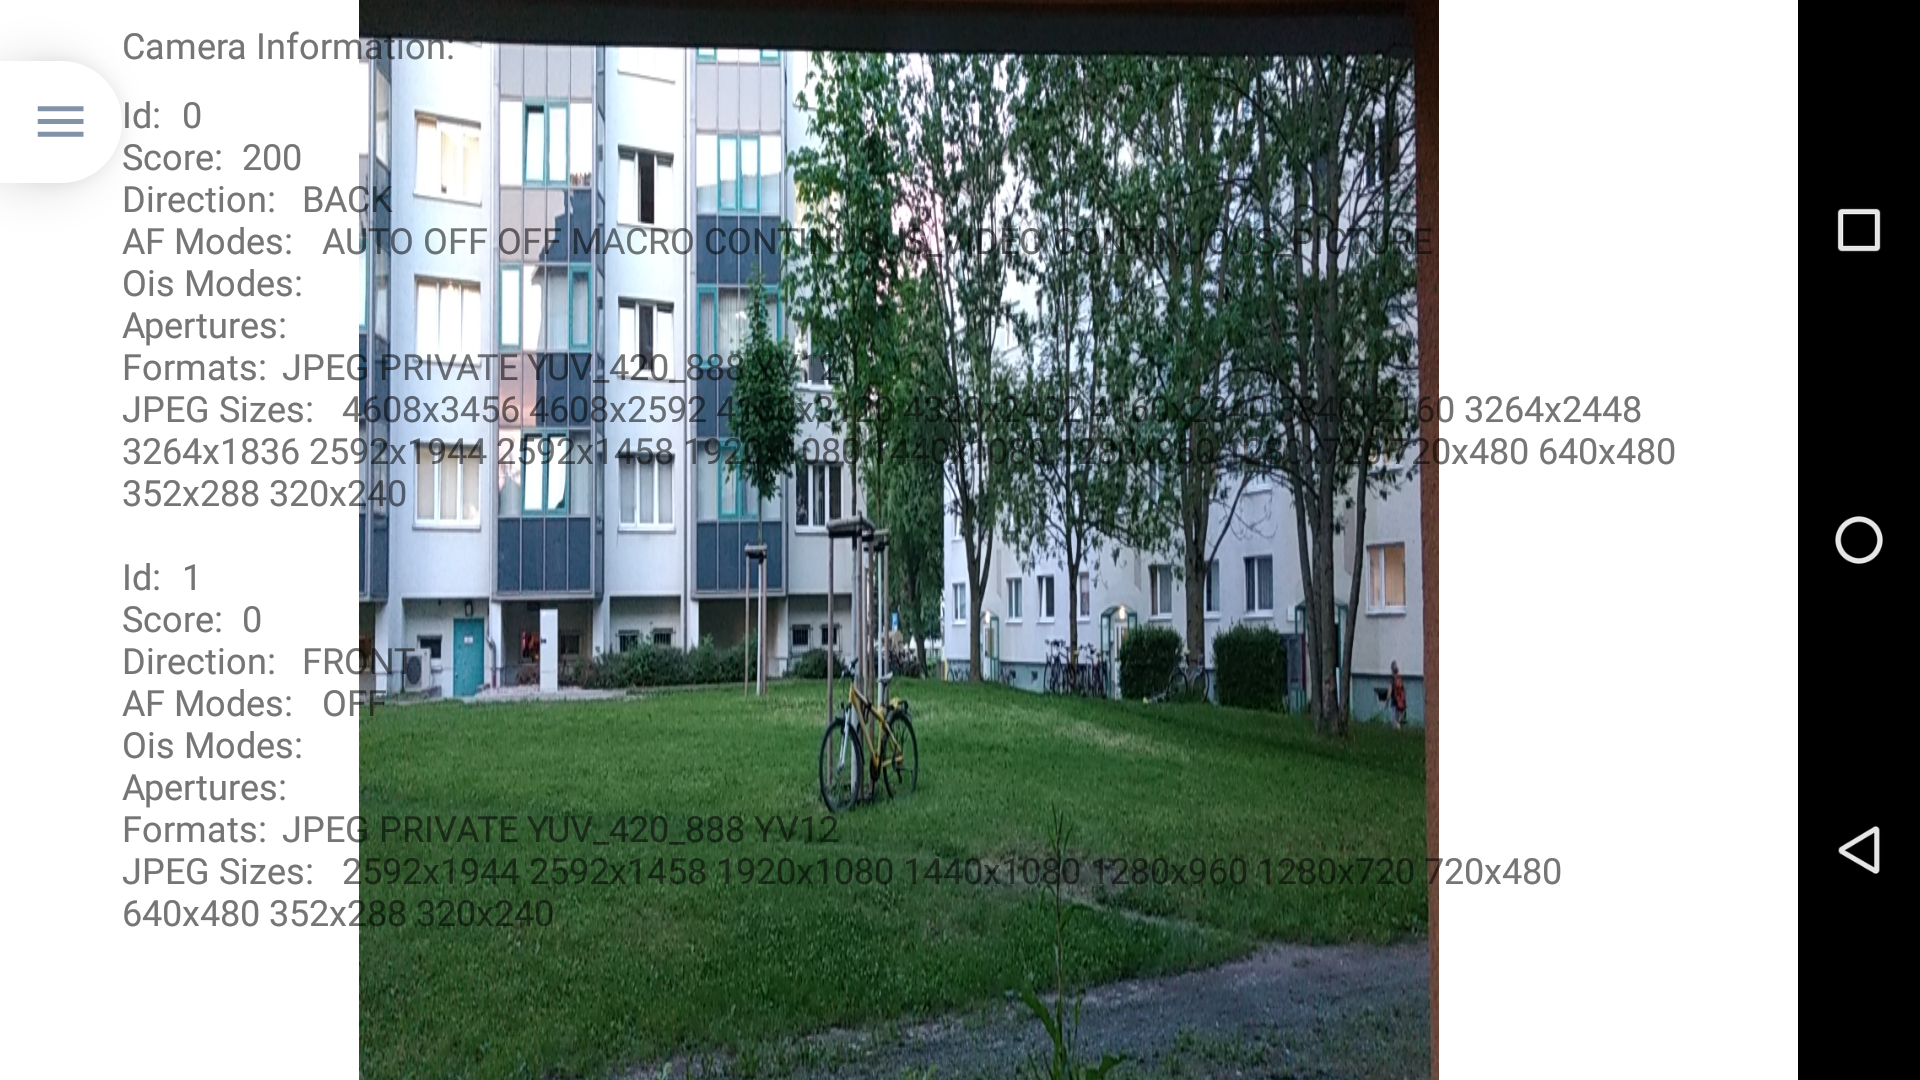
\includegraphics[width=0.9\linewidth]{Reviewdokument/Grafiken/app_debug_screenshot.png}
\caption{Debug-Fragment der App}
\label{fig:debug_ui}
\end{figure}

Die GPS-Geschwindigkeitsermittelung wurde ebenfalls fertiggestellt. Dabei wurde von der Methode \texttt{onLocationChanged()} des Android-Frameworks Gebrauch gemacht, welche automatisch aufgerufen wird, sobald das GPS eine Ortsänderung feststellt. Um die Geschwindigkeit zu errechnen, wird aus den GPS-Daten (Längen- und Breitengrad) die zurückgelegte Distanz in Meter bestimmt und durch die seit dem letzten Methodenaufruf vergangene Zeit dividiert. Erste Tests der GPS-Geschwindigkeitsermittelung im Vergleich mit einer Navigationsapp mit Geschwindigkeitsanzeige\footnote{\link{https://www.tomtom.com/de\_de/drive/sat-nav-app/go-mobile/}, 12.06.2018} zeigten, dass diese mit hinreichender Genauigkeit funktioniert. Um Ausreißer durch fehlerhafte Standortsermittelung zu vermeiden, werden die gemessenen Geschwindigkeiten in einer Datenstruktur ähnlich eines Ringspeichers geladen und die angezeigte Geschwindigkeit aus diesen gemittelt (Pflichtenheft P4304, B6007, B6009).\\

Da \glslink{Neuronales Netzwerk}{Neuronale Netze} oft sehr empfindlich auf Drehung des Eingaberaumes reagieren, ist es notwendig, dass das \gls{Smartphone} während der Fahrt möglichst waagerecht ausgerichtet ist. Dazu wurde in der \gls{App} ein Kalibrierungsmenü umgesetzt, was dem \gls{Nutzer} vermitteln soll, ob das \gls{System} korrekt kalibriert ist oder nicht (Pflichtenheft P4306). Zunächst war geplant, dies mit dem Drehvektorsensor\footnote{\link{https://developer.android.com/guide/topics/sensors/sensors\_motion\#sensors-motion-rotate}, 08.06.2018} umzusetzen, was sich aber als unnötig kompliziert erwies. Um aus dem Drehvektor die Neigung um die Y-Achse zu ermitteln, sind eine Reihe von Matrixoperationen notwendig, außerdem ist der Drehvektorsensor unter Umständen (z.B. wenn sich in der Nähe eine Magnetfeldquelle befindet) nicht besonders genau. Würde man sich für die Ausrichtung des \gls{Smartphone}s im Raum interessieren, wäre das die richtige Lösung gewesen. Für die Kalibrierung ist aber nur die Neigung um die Y- und Z-Komponente notwendig. Deshalb wurde sich für den G-Sensor\footnote{\link{https://developer.android.com/guide/topics/sensors/sensors\_motion\#sensors-motion-grav}, 08.06.2018} entschieden, wobei mittels einer Arkustangens-Berechnung die gesuchten Drehwinkel bestimmt werden. Das \gls{System} ist korrekt kalibriert, falls das \gls{Smartphone} jeweils nicht mehr als 5° um die \glslink{Drehachsen}{Nick- und Rollachse} gedreht ist. Das \gls{UI} des Setup-Menüs zu Ende der zweiten Iteration ist in \cref{fig:setup_ui} abgebildet.\\

Bei dem \gls{UI} wurde sich zunächst an das Mockup gehalten, wie aus \cref{fig:detektor_ui} ersichtlich ist. Damit das Layout aber übersichtlicher wird - insbesondere sollen keine UI-Elemente von dem aktuell erkannten Verkehrszeichen ablenken - wurde es jedoch noch einmal komplett überarbeitet. Der Fokus bei dem Redesign lag darauf, das \gls{UI} etwas lebhafter zu gestalten, aber gleichzeitig nicht so farbenfroh, dass es von den wichtigen Informationen ablenkt. Das zuletzt erkannte Verkehrszeichen soll weiterhin das \gls{UI} dominieren (Pflichtenheft B6001, B6002, B6003, B6004). \cref{fig:detektor_ui_neu} zeigt das neue \gls{UI}.\\

Des Weiteren wurde ein Warnhinweis beim Start der \gls{App} implementiert, welcher dem Nutzer vermittelt, dass die \gls{App} kein Ersatz für Aufmerksamkeit am Steuer ist und dass deren Anwendung nur innerhalb der geltenden StVO erfolgen darf(Pflichtenheft P4307).

\begin{figure}[H]
\centering
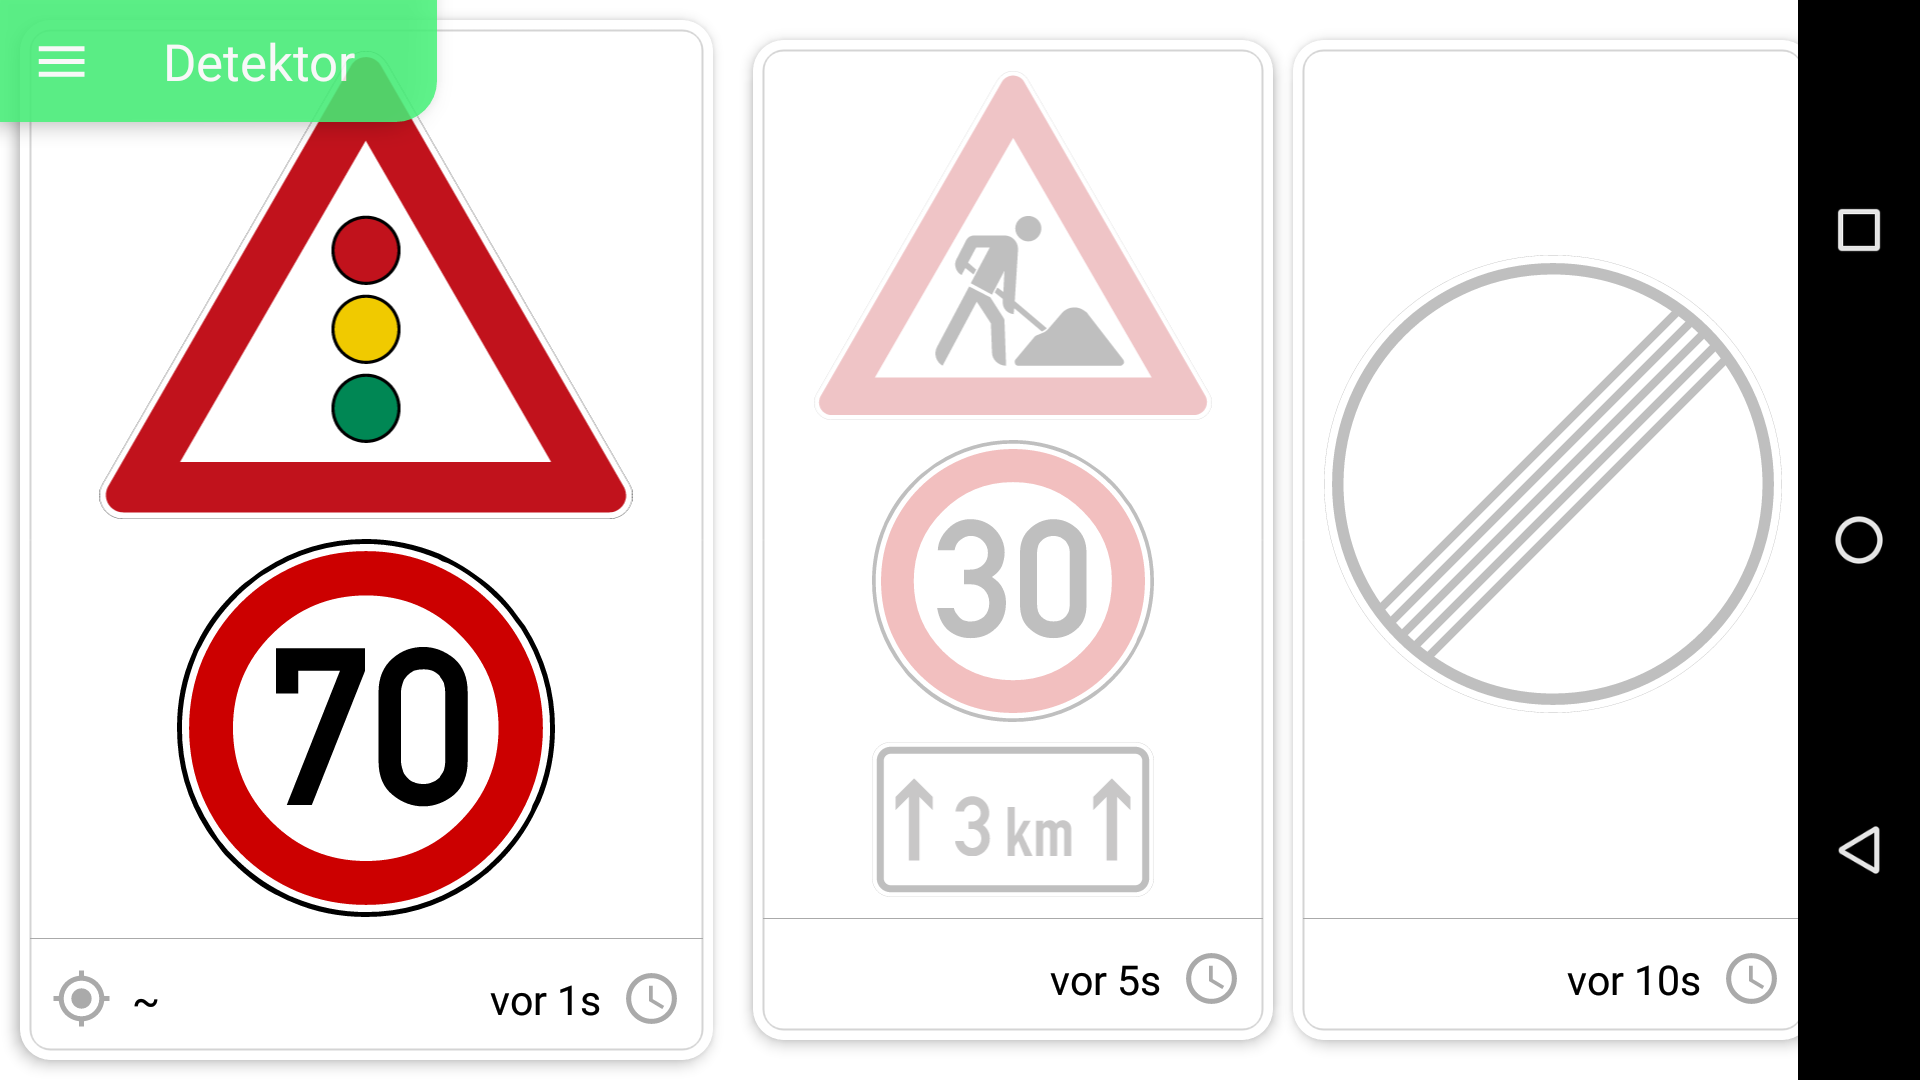
\includegraphics[width=0.9\linewidth]{Reviewdokument/Grafiken/app_detektor_neu.png}
\caption{UI des Detektor-Fragmentes zu Ende der zweiten Iteration}
\label{fig:detektor_ui_neu}
\end{figure}


\begin{figure}[H]
\centering
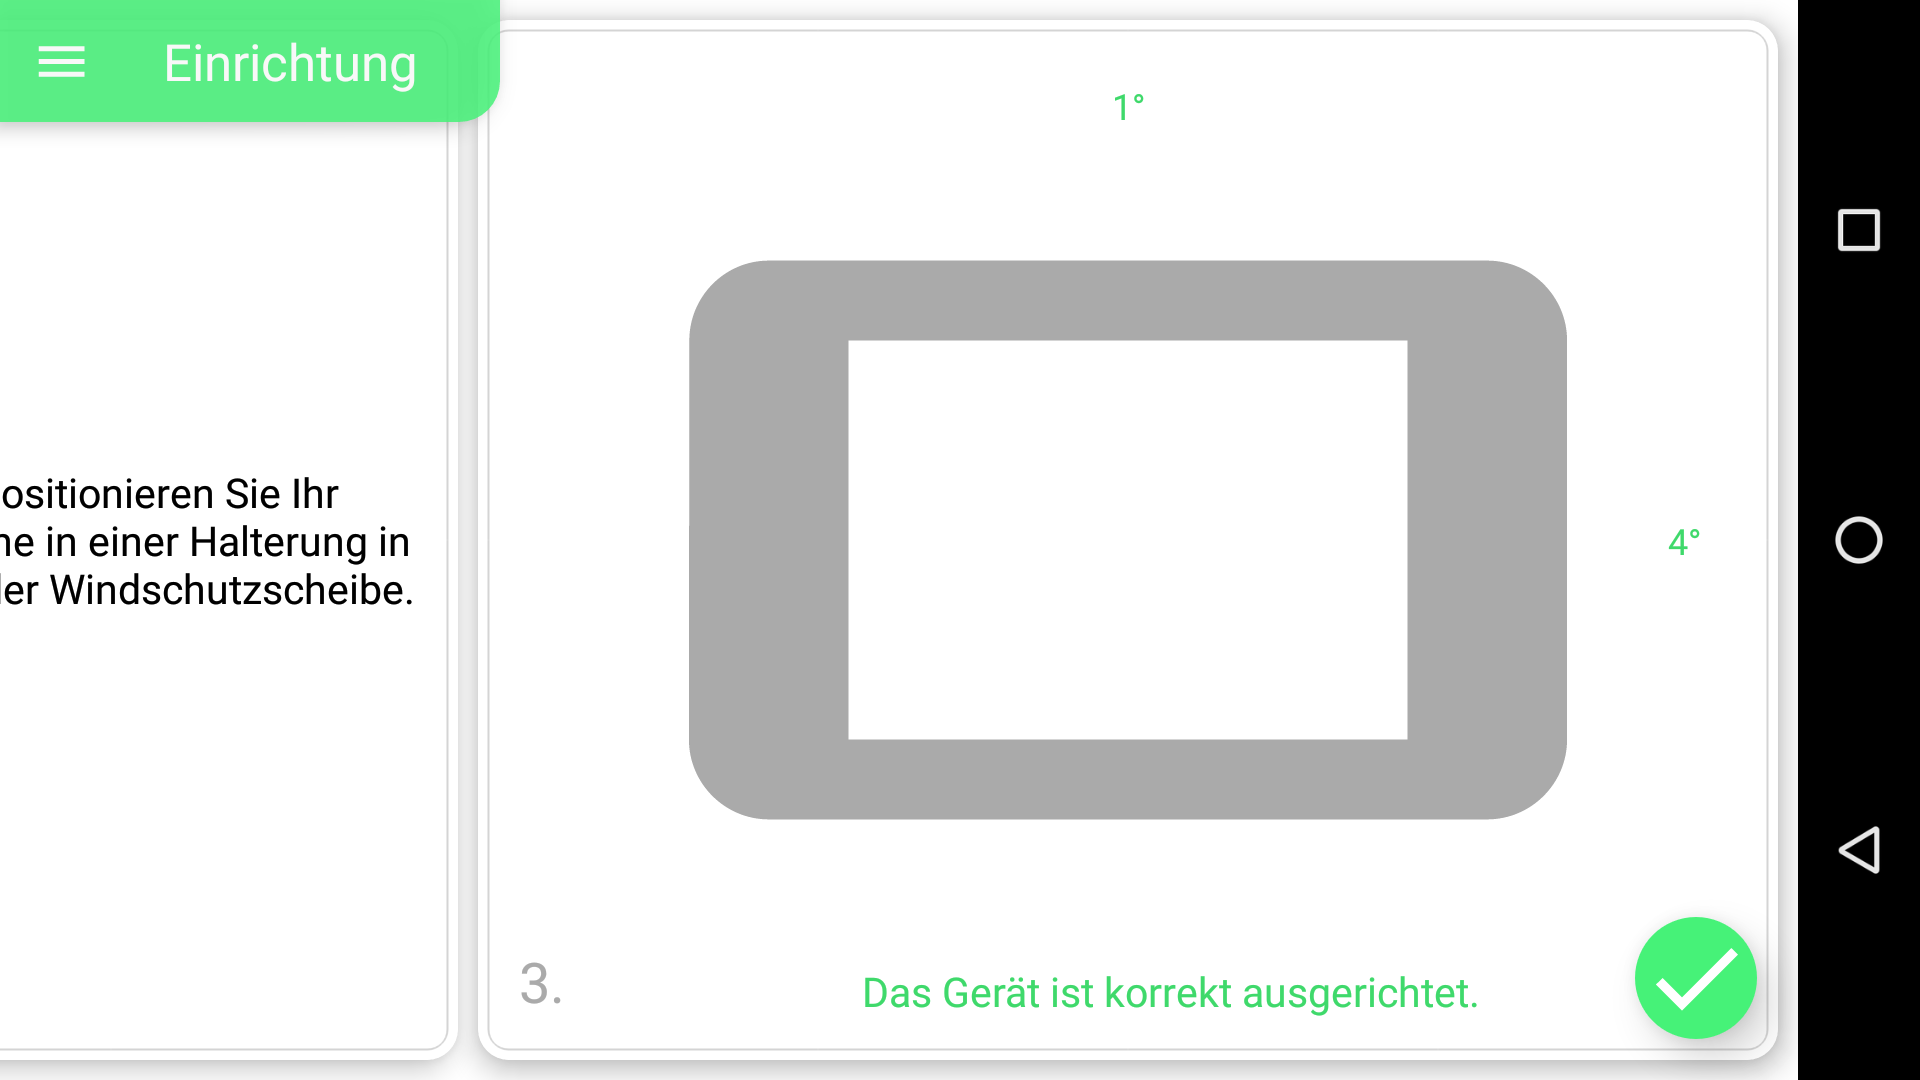
\includegraphics[width=0.9\linewidth]{Reviewdokument/Grafiken/app_setup_neu.png}
\caption{UI des Kalibrierungs-Fragmentes zu Ende der zweiten Iteration}
\label{fig:setup_ui}
\end{figure}

Das Kalibrierungsmenü zeigt dem \gls{Nutzer} nun neben der \glslink{Drehachsen}{Rollachse auch die Nickachse} an. Zwar sollte es für den \gls{Nutzer} selbstverständlich sein, dass das \gls{Smartphone} mit der Kamera in Fahrtrichtung zu zeigen hat, aber es ist für Nutzer möglicherweise nicht intuitiv entscheidbar, ob es eher auf die Fahrbahn, gerade nach vorn oder in Richtung Himmel zeigen muss.\\

\section[Meilenstein 4: Filterverwaltungs-Bibliothek]{Meilenstein 4: Filterverwaltungs-Bibliothek, bis 10.06. (200 PS)}
Dieser Meilenstein umfasst neben der Implementierung der \gls{Filterverwaltungs-Bibliothek} selbst auch die Schaffung der für die Entwicklung und Ausführung derselben benötigten Voraussetzungen (Pflichtenheft P4201, P4202, P4203, P5005). Da für die Verwaltung der \glslink{Neuronales Netzwerk}{Neuronalen Netze} TensorFlow verwendet werden und die Programmierung in C++ erfolgen sollte, war es zunächst notwendig, die entsprechenden Bibliotheken aus dem TensorFlow-Quellcode zu kompilieren. Dies geschah sowohl für Android als auch für x86-64 Linux (Ubuntu), um so ein Entwickeln auf beiden Plattformen zu ermöglichen, mit dem Ziel, die generelle Funktionsweise der \gls{API} und der \gls{Filterverwaltungs-Bibliothek} direkt aus der Entwicklungsumgebung heraus auf dem PC testen und verifizieren zu können. 
Hierbei ergaben sich einige Probleme (die mittlerweile weitgehend gelöst sind), welche im Folgenden kurz aufgelistet werden:\\

\subsubsection{Einbinden der TensorFlow-Header}
Um TensorFlow mit C++ benutzen zu können, werden die entsprechenden Header mit den Deklarationen der einzelnen Funktionen, Klassen, Structs und Enumerationen benötigt. Diese sind prinzipiell auch im Quellcode von TensorFlow verfügbar. Es ist allerdings nicht dokumentiert, welche Header genau benötigt werden und wie diese den Projekteinstellungen hinzuzufügen sind: einige der Header entstehen erst, nachdem TensorFlow das erste Mal kompiliert wurde und befinden sich in gänzlich anderen Ordnern, wo diese intuitiv nicht zu vermuten wären. Es gibt allerdings auch Fälle, in denen Platzhalter für die Header in die normale Ordnerstruktur eingepflegt sind, die sich darüber hinaus oft auch noch selbst einbinden, sodass Zirkelbezüge entstehen. Die Header aus dem Quellcode und jene, welche nach dem Kompilieren entstehen, müssen dann auf eine spezielle Weise in eigene Projekte eingebunden werden. Unterordner, die bereits als Teil eines übergeordneten Ordners eingebunden wurden, müssen teilweise selbst separat als \glqq{}Include Verzeichnis\grqq{} hinzugefügt werden, da unterschiedliche Teile von TensorFlow die einzelnen Dateien unterschiedlich einbinden. Dies war allerdings nicht dokumentiert und musste durch Studieren veröffentlichter Projekte (z.B. auf GitHub) sowie ausgiebigem Experimentieren herausgefunden werden.\\

\subsubsection{Kompilieren der Libraries}
Die Bibliotheken von TensorFlow mussten sowohl für \gls{ARM}-Android als auch für x86-64 Architekturen kompiliert werden. Hierbei kam es vor, dass sich die Bibliothek für einige der Architekturen, z.B. für arm64-v8a nicht erzeugen ließ. Dieses Problem konnte nur durch minutiöses experimentieren, verteilt über mehrere Rechner und Distributionen, gelöst werden, da die Dokumentation dazu, falls vorhanden, nicht öffentlich zugänglich ist.\\

\subsubsection{Unterschiedliche Ops auf ARM und x86-64}
\glqq{}Ops\grqq{} (Operations) im Sinne von TensorFlow sind Knoten im TensorFlow-Graphen, welche Berechnungen auf oder mit Tensor Objekten durchführen und selbst wieder beliebig viele Tensor Objekte zurückgeben, welche von anderen Ops benutzt werden können.
Da die zum Testen verwendete x86-64-Linux-Version anders als die \gls{ARM}-Version für Android kompiliert wird, kann es momentan noch zu Kompatibilitätsproblemen von verwendeten \glslink{Neuronales Netzwerk}{Neuronale Netzwerken} kommen.
Da eine lauffähige Android-Version priorisiert wird, und die Linux-Version, wie bereits angesprochen, nur zum Testen genutzt wird, liegt momentan der Fokus darauf, die richtigen Ops für Android einzubinden.\\
Jedoch wurde es geschafft, eine lauffähige Version für x86-64-Prozessoren mit AVX2 (Advanced Vector Extensions)-Support zu kompilieren. Dadurch ist ein Testen auf diesen Prozessoren möglich.\\

Während der Implementierung wurde festgestellt, dass einige, vor allem für die Detektion relevante, Ops, nicht von \gls{TensorFlow Lite} unterstützt werden. Um die Funktionalität dieser Neuronalen Netzwerke zu gewährleisten, musste deswegen ein Wechsel auf \gls{TensorFlow Mobile} vollzogen werden.\\
Nach dem Umstieg von \gls{TensorFlow Lite} auf \gls{TensorFlow Mobile} wurden wieder alle benötigten Abhängigkeiten erzeugt und eingebunden. Für die Entwicklung ist eine CMake-basierte Umgebung aufgesetzt worden. Die dynamische Bibliothek für die Android-\gls{App} wird dabei direkt aus Android Studio heraus erzeugt. Für Testzwecke wurde allerdings auch eine ndk-build Umgebung angelegt, mit derer sich der Code auch ohne Android Studio zu Testzwecken direkt kompilieren lässt.\\


\section[Meilenstein 5: Verkehrszeichen-API und Neuronale Netzwerke]{Meilenstein 5: Verkehrszeichen-API und Neuronale Netzwerke, bis 10.06. (290 PS)}
\subsection{Detektion}
Bei \glslink{Neuronales Netzwerk}{Neuronalen Netzwerken} zur Objektdetektion existiert stets ein Kompromiss zwischen Geschwindigkeit und Präzision. Es gibt eine Vielzahl verschiedener Architekturen, daher ist es notwendig, die Architektur des \glslink{Neuronales Netzwerk}{Neuronalen Netzwerkes} mit Bedacht auszuwählen und diese Faktoren für das gegebene Problem optimal zu gestalten. 

Diese Geschwindigkeit kann grob bestimmt werden, indem betrachtet wird, wieviele \gls{FLOPs} die Architektur benötigt.
Hierbei ist es wichtig zu wissen, dass Smartphones mit TensorFlow Mobile aktuell nur auf \gls{CPU}, nicht auf der leistungsstärkeren \gls{GPU}, rechnen können.
Die \gls{FLOPS} von Smartphone-\gls{CPU}s ist generell eher niedrig, weswegen es absolut entscheidend ist, dass die \gls{Detektion} möglichst wenig \gls{FLOPs} benötigt um diese videotaktschritthaltend zu ermöglichen.

Jedoch ist für eine genaue \gls{Detektion} eine hohe Anzahl von \gls{FLOPs} vonnöten, um feinere Merkmale zu extrahieren. Wird die \glslink{FLOPs}{FLOP}-Zahl zugunsten der Geschwindigkeit gering gehalten, sorgt dies für eine Abnahme der Präzision.
In der folgenden Betrachtung wird der Kompromiss dargestellt.
Bei den getesteten \glslink{Neuronales Netzwerk}{Neuronalen Netzwerken} handelt es sich um auf den COCO-Datensatz\footnote{\link{http://cocodataset.org/}, 31.05.2018} trainierte Netzwerke, deren Gewichte frei verfügbar sind.\\
\newcounter{n}
\setcounter{n}{\value{footnote}}

\clearpage
\begin{longtabu}{|l|r|r|r|r|}
\hline
Architektur & verwendete Auflösung & geteste Laufzeit\footnotemark & \gls{FLOPs} & \gls{mAP}\footnotemark \\
\hline
Tiny YOLO v1\cite{DBLP:journals/corr/RedmonDGF15} & 448$\times$448 & 508.71 ms $\pm$ 43.35 ms & \num{4.50e9} & - \\
Tiny YOLO v2\cite{DBLP:journals/corr/RedmonF16} & 416$\times$416 & 621.04 ms $\pm$ 74.71 ms & \num{5.41e9} & 23.7\\
Tiny YOLO v3\cite{DBLP:journals/corr/abs-1804-02767} & 416$\times$416 & (nicht getestet) & \num{5.56e9} & 33.1 \\
SSDLite\cite{DBLP:journals/corr/abs-1801-04381} &300$\times$300 & 295.02 ms $\pm$ 28.05 ms & \num{1.50e9} & 22.0 \\
\hline
\end{longtabu}
\setcounter{footnote}{\value{n}}

Die verwendete Vergleichsgröße \textit{Mean Average Precision} (mAP) ist ein gängiges Maß zur Bewertung der Präzision von Objektdetektionsnetzwerken. Grundlegende Faktoren der Berechnung stellen die Abweichung der vorhergesagten Bounding Box von der gegebenen sowie die Zuordnung zur korrekten Klasse dar. Damit die Evaluierung repräsentativ ist, wird dies auf einem Teil des Datensatzes berechnet, welcher explizit nicht für das Training verwendet wurde.
Diese Tatsache ist wichtig, da das Netzwerk sonst den unfairen Vorteil hätte, die Bilder bereits gelernt zu haben. Dies würde keine zielführende Auswertung liefern, da das Netzwerk in einem realen Einsatz auch ohne spezifisch gelernte Verkehrszeichen klar kommen muss.\\
\footrealtext{Durchschnittliche Berechnungszeit auf einem \gls{Smartphone} mit Snapdragon-820-Prozessor.}
\footlinktext{http://homepages.inf.ed.ac.uk/ckiw/postscript/ijcv\_voc09.pdf}{30.05.2018}
\footlinktext{https://pjreddie.com/darknet/yolo/}{30.05.2018}


SSDLite\cite{DBLP:journals/corr/abs-1801-04381} benötigt mit Abstand von ca. 250 ms die geringste Zeit pro Eingabe und bietet dabei eine \gls{mAP}, welche der Präzision von Tiny YOLO v2\cite{DBLP:journals/corr/RedmonF16} nahe kommt und einen guten Kompromiss darstellt. Durch die deutlich geringere Rechenzeit, können mehr Frames pro Sekunde verarbeitet werden. Dadurch haben nicht oder falsch detektierte Verkehrszeichen, sofern sie in späteren Frames erneut auftauchen, eine weitere Chance korrekt detektiert zu werden.\\
Einen Nachteil bringt SSDLite\cite{DBLP:journals/corr/abs-1801-04381} mit sich, wenn es um die Auflösung geht. Ein Teil der Rechenzeit wird eingespart, indem kleinere Bilder als Eingabe für das \glslink{Neuronales Netzwerk}{Neuronale Netzwerk} verwendet werden.
Eine Auflösung von 300$\times$300 erfordert, dass die Bilder noch kleiner skaliert werden als z.B. bei Tiny YoloV2\cite{DBLP:journals/corr/RedmonF16}.
Durch die Skalierung werden die Verkehrszeichen noch kleiner skaliert und sind schwieriger in dem Bild zu erkennen.\\
Es wurde sich, trotz der deutlich höheren \gls{mAP}, bewusst gegen Tiny YOLO V3\cite{DBLP:journals/corr/abs-1804-02767} entschieden.
Dies liegt daran, dass es aktuell noch keine Implementierung gibt, welche mit TensorFlow funktioniert.
Eine eigene Implementierung hätte Zeit in Anspruch genommen, weswegen auf das Testen verzichtet wurde.
Jedoch benötigt diese Architektur noch mehr FLOPs als Tiny YOLO v2\cite{DBLP:journals/corr/RedmonF16}, weswegen wir von einer leicht höheren Rechenzeit ausgehen.

Aufgrund dieser Argumente wurde sich für Verwendung von SSDLite\cite{DBLP:journals/corr/abs-1801-04381} entschieden, da es den besten Kompromiss zwischen Geschwindigkeit und Präzision für das Projekt bietet.\\
\\
Bei dem Training des \glslink{Neuronales Netzwerk}{Neuronalen Netzwerks} haben sich Probleme bemerkbar gemacht. Da der in Meilenstein 6.2. erstelle Datensatz relativ unbalanciert ist (d.h.: einige Verkehrszeichen kommen deutlich häufiger vor als andere), war es für das Netzwerk nicht möglich, die seltenen Klassen zu lernen. Um dieses Problem zu lösen, wurden Gewichtungen für die einzelnen Klassen eingeführt, welche bewirken sollen, dass die selten vorkommenden Klassen mehr gelernt werden als jene, die häufigen vorkommen. Dies berücksichtigt jedoch nicht, wie gut das Netzwerk die einzelne Klasse bereits beherrscht.
Deswegen sollten die einzelnen Klassengewichte gut gewählt werden.
%Dies hat sich auch nach erneutem Lernen durch sehr schlechte \glslink{Detektion}{Detektionsergebnisse} bemerkbar gemacht.\\
Ein weiteres Problem ist mit der eigentlichen Aufgabe des Dektektors verbunden. Dieser muss in der Lage sein, Verkehrszeichen verschiedener Klassen in einem Bild detektieren zu können. Dies ist bei Neuronalen Netzwerken nicht immer der Fall. Das verwendete Neuronalen Netzwerk hat mehrere Ausgabeneuronen zur Repräsentation der einzelnen Klassen und verwendet die Kategorische Kreuzentropie Loss-Funktion, welche mit solchen \glqq{}Multilabel\grqq{}-Problemen gut umgehen kann. Bei einer genaueren Betrachtung der vorliegenden Probleme wurde ein Wechsel auf die Funktion \textit{\glqq{}Focal Loss\grqq{}} \cite{DBLP:journals/corr/abs-1708-02002} als sinnvoll erachtet. Diese ist eine speziell für \glslink{Detektion}{Detektionsnetzwerke} entwickelte Funktion, welche bisher schlecht gelernte Klassen, oder sogar Einzelbilder aus einer Klasse, stärker gewichtet als schon gut gelernte Beispiele. Ein Vergleich der beiden Loss-Funktionen befindet sich in \cref{fig:lossfunktionen}.\\
\begin{figure}[H]
\centering
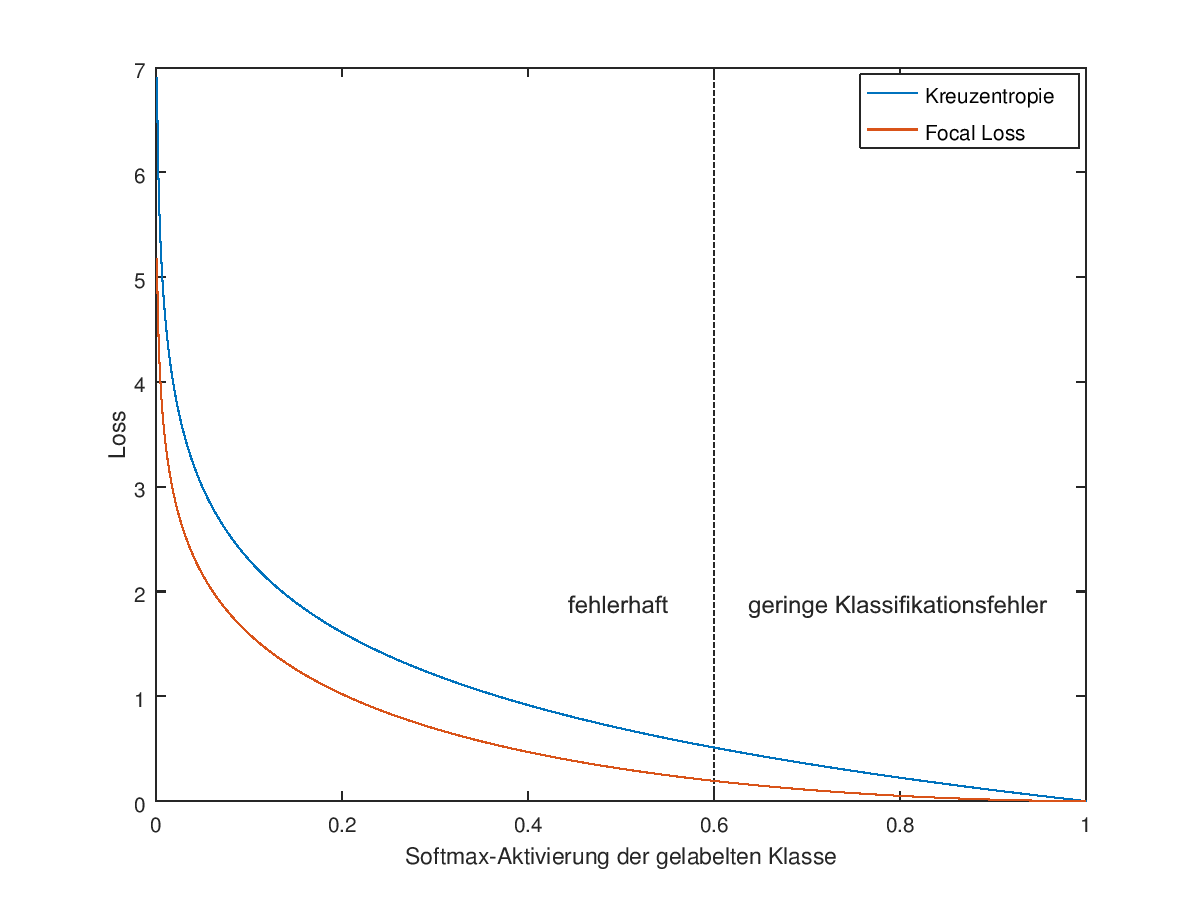
\includegraphics[width=1.1\linewidth]{Grafiken/lossfunktionen.png}
\caption{Vergleich der beiden Loss-Funktionen}
\label{fig:lossfunktionen}
\end{figure}

Diese Funktion besitzt zwei einstellbare Parameter, mit welchen festgelegt werden kann, wie viel stärker die schwachen \gls{Sample}s gewichtet werden. \cite{DBLP:journals/corr/abs-1708-02002} Hierbei ist es wichtig, einen guten Mittelweg zu wählen. Bei zu klein gewählten Parametern würde die Funktion die schwachen Klassen zu wenig beeinflussen. Wenn die Parameter jedoch zu groß gewählt sind, wird sogenanntes \glqq{}Overfitting\grqq{} betrieben, welches vermieden werden sollte, da dieses zu einer zu starken Spezialisierung des Neuronalen Netzwerkes auf die Trainingsdaten führen kann.\\
Daher hält sich diese Implementierung an die Empfehlung der Publikation \cite{DBLP:journals/corr/abs-1708-02002}, die sich mit einer ähnlichen Problemstellung beschäftigt\\


Zusätzlich wurden schon bei der Detektion deutlich mehr Einzelklassen angelernt. So wurden statt den vorher verwendeten drei Klassen (geschwindigkeitsregulierende \gls{VZ}, Zusatzzeichen, sonstige \gls{VZ}) insgesamt fünfzehn Klassen(\cref{sec:klassen_detektion})
eingeführt. Vor allem die \glqq{}Sonstige Verkehrszeichen\grqq{} Klasse, welche die Mehrheit der gesamten Daten darstellte, wurde in mehrere Klassen aufgeteilt wie z.B. \glqq{}Verschiedene Gelb\grqq{}, \glqq{}Verschiedene Blau\grqq{} oder \glqq{}Verschiedene Grün\grqq{}.\\
Nach einem erneuten Training haben sich deutlich bessere \glslink{Detektion}{Detektionsergebnisse} feststellen lassen. Fast alle Verkehrszeichen wurden beim Testen erkannt. Ab und zu liegen diese jedoch noch in der falschen Klasse, was sich mit der geringen Auflösung von 300$\times$300 Pixeln in Verbindung bringen lässt. Deswegen sollte die Ausgabe der Klasse eher als \glqq{}Guess\grqq{} (Vermutung) betrachtet werden und generell nochmal in einer höheren Auflösung durch das \glslink{Klassifikation}{Klassifikatornetzwerk} ausgewertet werden.\\

\subsection{Klassifikation}
Bei \glslink{Neuronales Netzwerk}{Neuronalen Netzen} zur \gls{Klassifikation} besteht ebenfalls der Kompromiss zwischen Geschwindigkeit und Präzision. Es gibt wenige Architekturen, welche für \glslink{Smartphone}{Smartphones} ausgelegt sind: zum Beispiel MobileNetV1\cite{DBLP:journals/corr/HowardZCKWWAA17} , MobileNetV2\cite{DBLP:journals/corr/abs-1801-04381}  und NASNet-Mobile. Diese Modelle klassifizieren Bilder in sehr kurzer Zeit und haben für die Geschwindigkeit eine ausreichende Genauigkeit.\\

\begin{tabu}{|X[l]|r|r|r|}
\hline
Architektur & verwendete Auflösung & Top 1 Accuracy & CPU Laufzeit \\
\hline
MobileNetV1\cite{DBLP:journals/corr/HowardZCKWWAA17}    & 244$\times$244 & 70.6 & 113 ms \\
NasNet-A-Mobile & 244$\times$244 & 74.0 & 183 ms \\
MobileNetV2\cite{DBLP:journals/corr/abs-1801-04381}    & 244$\times$244 & 72.0 & 75 ms \\
MobileNetV2\cite{DBLP:journals/corr/abs-1801-04381}  &  96$\times$96\footnotemark[9] & 60.3 & 18 ms \\
\hline  
\end{tabu}~\\
Die Tabelle vergleicht die genannten Architekturen hinsichtlich Top-1-Accuracy und Rechenzeit. Die Top-1-Accuracy gibt an, wie viel Prozent der Netzwerkausgaben mit der höchsten Wahrscheinlichkeit mit den geforderten Ausgaben übereinstimmen. Dabei ist zu beachten, dass die Netzwerke auf den Imagenet\footnotemark[10]-Datensatz mit 1001 verschiedenen Klassen und auf der \gls{CPU} eines Google Pixel 1 getestet wurden.\\

\footlinktext{https://github.com/tensorflow/models/tree/master/research/slim/nets/mobilenet}{12.06.2018}
\footlinktext{www.image-net.org/}{12.06.2018}

Beim Vergleich der genannten Architekturen unter der gleichen Auflösung der zu klassifizierenden Bilder stellte sich heraus, dass MobileNetV2\cite{DBLP:journals/corr/abs-1801-04381} eine viel kürzere Rechenzeit als NasNet-A-Mobile und eine etwas kürzere Rechenzeit als MobileNetV1\cite{DBLP:journals/corr/HowardZCKWWAA17}, wobei nur eine geringfügig schlechtere Genauigkeit als NasNet-A-Mobile und sogar eine bessere Genauigkeit als MobileNetV1\cite{DBLP:journals/corr/HowardZCKWWAA17} aufweist.
Die Geschwindigkeit der Netzwerkarchitekturen kann darüber hinaus noch gesteigert werden, wenn man eine Architektur wählt, welche für kleinere Bildgrößen konzipiert ist. 
So gibt es Netzwerkarchitekturen für kleinere Auflösungen bis hin zu 128$\times$128 für MobileNetV1\cite{DBLP:journals/corr/HowardZCKWWAA17} und 96$\times$96 für MobileNetV2\cite{DBLP:journals/corr/abs-1801-04381}.
Theoretisch würden zum Klassifizieren von Verkehrszeichen eine Bildgröße von 40$\times$40 für das menschliche Auge und somit auch für ein \glslink{Neuronales Netzwerk}{Neuronales Netzwerk} ausreichen, allerdings ist MobileNetV2\cite{DBLP:journals/corr/abs-1801-04381} in der 96$\times$96 Version das Modell mit vortrainierten Gewichten mit der kleinsten Auflösung.
Da die Klassifikation innerhalb kürzester Zeit und mit guter Genauigkeit erfolgen soll, fiel die Wahl der Architektur auf MobileNetV2\cite{DBLP:journals/corr/abs-1801-04381}.\\
Weiterhin war uns wichtig, vortrainierte Modelle zu verwenden, da diese, obwohl sie auf einen anderen Datensatz trainiert wurden, grundlegende Merkmale wie beispielsweise Kanten in einem Bild erkennen können, was den Trainingsprozess beschleunigt. Für MobileNetV2\cite{DBLP:journals/corr/abs-1801-04381} gibt es vortrainierte Modelle, welche auf den Imagenet Datensatz trainiert wurden.\\
Beim Training des Netzwerkes muss darauf geachtet werden, dass der gesammelte Datensatz nicht gut balanciert ist. Es gibt Verkehrszeichen, welche sehr häufig vertreten sind und es gibt kaum vertretene Verkehrszeichen.
Damit das \glslink{Neuronales Netzwerk}{Netzwerk} lernt, Verkehrszeichen zu klassifizieren, welche nur in geringen Mengen im Datensatz enthalten sind, kann man mit Klassengewichten trainieren, wie dies auch beim \glslink{Detektion}{Detektor} der Fall war.\\
%Das \glslink{Neuronales Netzwerk}{Netzwerk} zur \gls{Klassifikation} konnte unter anderem aufgrund von fehlender Rechenleistung und Fehleinschätzung der Datensatzaufbereitung noch nicht vollständig trainiert werden, was allerdings zu Beginn der nächsten Phase nachgeholt wird.\\

\section[Meilenstein 6: App-API-Anbindung]{Meilenstein 6: App-API-Anbindung, bis 14.06. (30 PS)}
Die \gls{Smartphone}-Kamera kann unterschiedliche Bildformate bereitstellen. Auf allen Smartphones, welche wenigstens die Android-\gls{API} Version 24 unterstützen, steht dabei das YUV\_420\_888 Format zur Verfügung, welches darüber hinaus auch in der offiziellen Dokumentation der Android-Kamera-\gls{API} zur Bildverarbeitung empfohlen wird. Da die von uns verwendeten Netzwerke RGB-Bilder benötigen und auch nur auf solchen trainiert wurden, musste eine Konvertierung des YUV-Formates in ein RGB-Format erfolgen. Im Detail sei dies in der Schnittstellendokumentation des Feinentwurfes aus Phase II genauer erläutert. Anschließend erfolgte die Einbindung der API relativ problemlos, zumindest nachdem die entsprechenden TensorFlow-Libraries für die \gls{ARM}-Architektur erfolgreich kompiliert wurden. Der Code der \gls{Filterverwaltungs-Bibliothek} und \gls{Verkehrszeichen-API} ist vor allem deswegen portabel, weil TensorFlow selbst weitgehend plattformunabhängig entwickelt wurde. Die bereits auf x86-64 lauffähige \gls{API} wurde als dynamische Bibliothek kompiliert, in die Android-\gls{App} eingebunden und über die entsprechenden Funktionen des Java Native Interfaces angesprochen.\\
Resümierend lässt sich sagen, dass die angestrebten Funktionalitäten entsprechend umgesetzt wurden: die \gls{App} ist in der Lage, Verkehrszeichen auf von der Kamera aufgenommenen Bildern zu \glslink{Detektion}{detektieren} und zu \glslink{Klassifikation}{klassifizieren} (sofern die dazu benötigten \glslink{Neuronales Netzwerk}{Neuronalen Netzwerke} bereitgestellt werden) und verwendet dafür die \gls{Verkehrszeichen-API}, welche wiederum auf der \gls{Filterverwaltungs-Bibliothek} aufbaut.

% -----------------------------------------

\part{Projektfortschritt, Phase III}

\chapter{Änderungen an der Implementierung}

\section{Änderungen an der Implementierung der App}

\subsection{Warnung bei zu geringer Leistung des Gerätes}
Es wurden Berechnungen zur Bestimmung jeder Geschwindigkeit implementiert, mit welcher ein Verkehrszeichen noch garantiert für mindestens einen Frame bearbeitet werden kann - also die höchste Geschwindigkeit, für welche die Verkehrszeichenerkennung noch verlässlich funktionieren sollte. Für eine Rechenzeit von 300 ms pro Frame beträgt diese Geschwindigkeit in etwa den im Pflichtenheft spezifizierten 150 km/h, bis zu denen das \gls{System} noch funktionieren soll.\\
Außerdem fiel während des Testens auf, dass das \gls{Smartphone} nach einer gewissen Zeit über\-hitzte und die \gls{CPU}-Leistung drosselte. Allerdings ist es einem \gls{App}-Entwickler unter normalen Gegebenheiten nicht möglich, das Betriebssystem dazu zu zwingen, diese Drosselung zu unterlassen.\\
Aufgrund des hohen Berechnungsaufwandes beim Verwenden \glslink{Neuronales Netzwerk}{Neuronaler Netzwerke} kann das Problem aus Sicht der Entwickler nur durch ein performanteres Netzwerk behoben werden, wobei die Kombination aus SSD Lite zur \gls{Detektion} und MobileNetV2 zur \gls{Klassifikation} bereits das schnellste darstellt, was gegenwärtig umsetzbar ist. Um dennoch dem \gls{Nutzer} mitzuteilen, dass sein \gls{Smartphone} für die aktuell gefahrene Geschwindigkeit zu langsam rechnet, wurde eine Funktion implementiert, die dem Nutzer eine entsprechende Warnung ausgibt, wie in \cref{fig:smartphone_zu_langsam} zu sehen ist.\\

\begin{figure}[H]
\centering
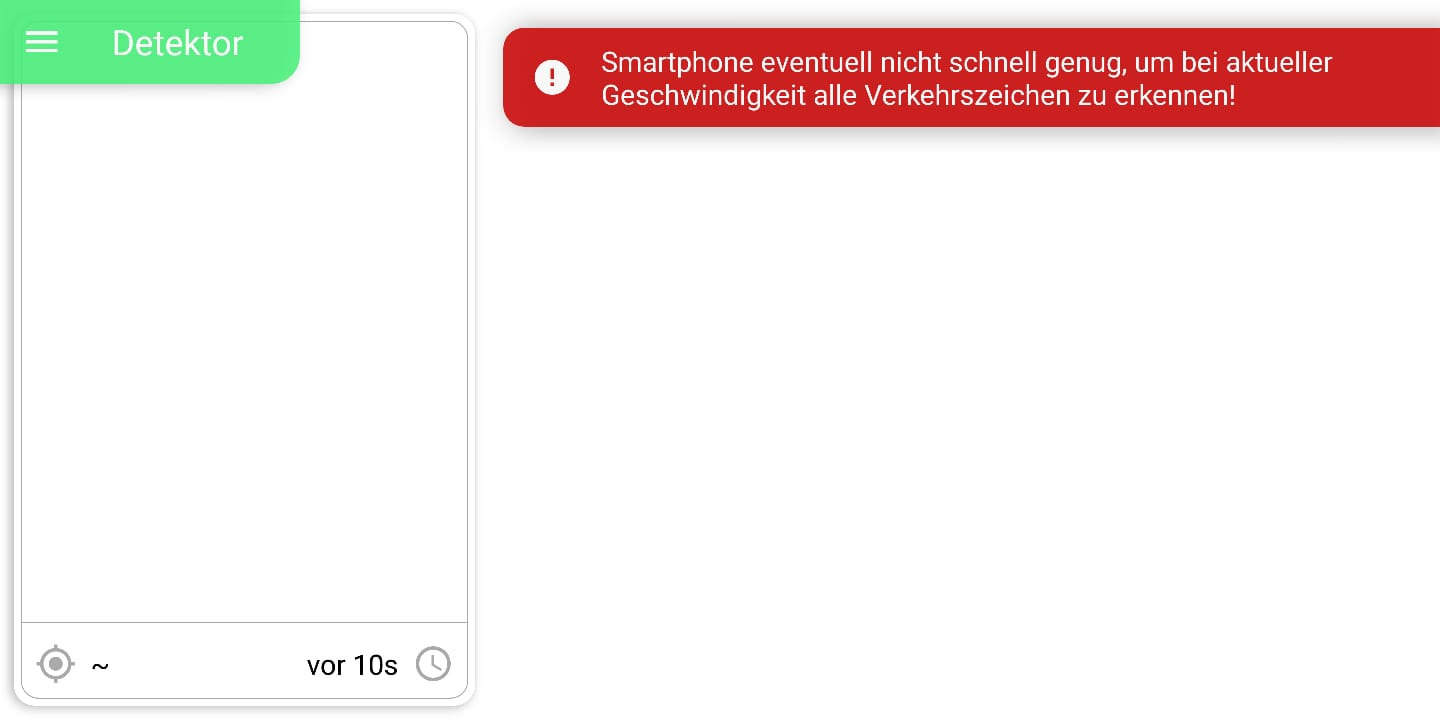
\includegraphics[width=0.9\linewidth]{Reviewdokument/Grafiken/smartphone_zu_langsam.jpeg}
\caption{Warnung bei zu geringer Rechenleistung}
\label{fig:smartphone_zu_langsam}
\end{figure}
\smallskip

\subsection{Erstellung eines About-Menüs}
Da die \gls{App} auch im Google Play Store\footnote{\link{https://play.google.com/store}, 25.06.2018} verfügbar sein soll, war es nötig, dass man rechtlich in mehrerlei Hinsicht abgesichert ist. So müssen beispielsweise die verwendeten OpenSource-Lizenzen sowie eine Datenschutzerklärung in der \gls{App} enthalten sein, damit man sie ohne Verstöße gegen das Urheberrecht und den Datenschutz veröffentlichen kann. Außerdem befindet sich dort noch einmal der Haftungsauschluss sowie ein Vermerk zur Kontaktaufnahme mit den Entwicklern.\\
Dieses Detail ist zwar an sich keine Implementierung in engeren Sinne, aber es ist dennoch absolut unabdingbar, um die App veröffentlichen zu können.\\

\subsection{Verhindern der automatischen Bildschirmdimmung}
Wenn das \gls{Smartphone} eine Weile nicht benutzt wird, d.h. der Bildschirm nicht berührt wird, wird dieser automatisch gedimmt und, den Geräteeinstellungen gemäß, irgendwann abgeschaltet. Natürlich würde das die Benutzbarkeit der \gls{App} in diesem Fall stark einschränken. Um den Bildschirm ständig aktiv zu halten, musste lediglich ein Flag (\texttt{FLAG\_KEEP\_SCREEN\_ON}) gesetzt werden.\\

\subsection{Verbesserung der Geschwindigkeitsermittlung}
\label{subsec:verbesserung-geschwindigkeitsermittlung}
Der Algorithmus zur Berechnung der Momentangeschwindigkeit aus der zweiten Phase basierte auf einer Speicherung der zuletzt berechneten Geschwindigkeiten, aus welchen für die Anzeige der einfache Durchschnitt ermittelt wurde.\\
Der neue Algorithmus speichert nun die zuletzt ermittelten Gerätepositionen mit den dazugehörigen Zeitpunkten. Zur Anzeige wird zunächst jene Position gesucht, welche sich am weitesten von allen anderen entfernt befindet. Diese wird dann in den nachfolgenden Schritten ausgelassen. Zwischen den verbleibenden Positionen werden die Teilgeschwindigkeiten berechnet. Die approximative Momentangeschwindigkeit ergibt sich dann aus dem Durchschnitt dieser Teilgeschwindigkeiten.\\
Der Vorteil dieser Implementierung liegt in der konstanteren angezeigten Geschwindigkeit bei konstanter realer Bewegung im Vergleich zum zuerst implementierten Algorithmus.\\

\subsection{Zusammenfassen (teil-)wiederholter Verkehrszeichenkombinationen}
Die Erkennung von Verkehrszeichen durch die \gls{API} erfolgt auf Basis eines einzelnen Bildes ohne Wissen über zuvor erkannte Informationen. Dadurch tritt häufig der Fall ein, dass eine \gls{Verkehrszeichenkombination} komplett oder zu Teilen mehrfach der App übergeben wird. Eine wiederholte Darstellung schränkt allerdings die Gesamtübersicht über die zuletzt erkannten Verkehrszeichen in der \gls{App} ein und ist somit zu vermeiden.\\
Deshalb werden nun neu erkannte \glslink{Verkehrszeichenkombination}{Verkehrszeichenkombinationen} mit den bereits erkannten und in der \gls{App} gespeicherten verglichen. Werden dabei Parallelen zu \glslink{Verkehrszeichenkombination}{Kombinationen} aus dem gleichen oder den letzten zwei analysierten Bildern gefunden, dann werden die Informationen bei Bedarf zu einer neuen \glslink{Verkehrszeichenkombination}{Kombination} zusammengefügt und diese anstelle jener von der \gls{API} übergebenen in der \gls{App} gespeichert. Beim Zusammenfügen wird dabei beachtet, dass möglichst neue Informationen erhalten bleiben, solange absehbar ist, dass dadurch die Korrektheit der dargestellten \gls{Verkehrszeichenkombination} nicht beeinflusst wird.\\
Eine Parallele zwischen zwei \glslink{Verkehrszeichenkombination}{Kombinationen} besteht genau dann, wenn die einzelnen Verkehrszeichen in der Art, Reihenfolge und Anzahl entweder genau übereinstimmen, oder wenn die Zeichen einer Kombination in der gleichen Reihenfolge unter der Möglichkeit von  Einschüben auch in der anderen vorhanden sind.\\

\subsection{Name der App}
Nach gut zweimonatiger Entwicklung wurde die \gls{App} auf den Namen \textit{Signapse} getauft - ein Wortspiel aus \textit{Sign} und \textit{Synapse}.\\

\section{Änderungen an der Implementierung der API}

\subsection{Fehlerhafte Mehrfachdetektionen}
Es ist aufgefallen, dass gelegentlich dasselbe Verkehrszeichen in demselben Bild fälschlicher\-weise mehrfach mit einem kleinen Versatz \glslink{Detektion}{detektiert} wird (sh. \cref{fig:mehrfachdetektion}), was für den \gls{Nutzer} natürlich störend ist, da es dann mehrfach in der Historie der App angezeigt würde. Außerdem würde so unnötig Rechenleistung durch die anschließende \gls{Klassifikation} verschwendet werden. Die Lösung bestand darin, dass die durch den \glslink{Detektion}{Detektor} gesetzten Boxen verglichen werden. In der \gls{Verkehrszeichen-API} wurde ein neuer Filter, der sog. \texttt{RoadSignDuplicationDeleter}-Filter, angelegt, welcher ebenjene Boxen vergleicht und im Falle überlappender Boxen eine der beiden verwirft. Als Schwellwert wurden dabei 60\% gewählt - ein \gls{Detektion}sergebnis wird also ignoriert, wenn mindestens 60\% seiner Fläche bereits von einem anderen \gls{Detektion}sergebnis beschrieben werden.\\

Eine Vermeidung dieser Mehrfachdetektionen ist zwar auch durch weiteres Training der \glslink{Neuronales Netzwerk}{Neuronalen Netzwerke} möglich, aber vollständig ausgeschlossen werden kann es nicht. Eine Erhöhung des Thresholds, ab welchem ein \gls{Detektion}sergebnis an den \glslink{Klassifikation}{Klassifikator} übergeben wird, hätte zur Folge, dass ggf. andere Verkehrszeichen gar nicht übergeben werden, obwohl sie eigentlich korrekt \glslink{Detektion}{detektiert} wurden. Die Verwendung eines Filters ist unter Betrachtung der Umstände die sinnvollste Alternative.\\

\begin{figure}[H]
\centering
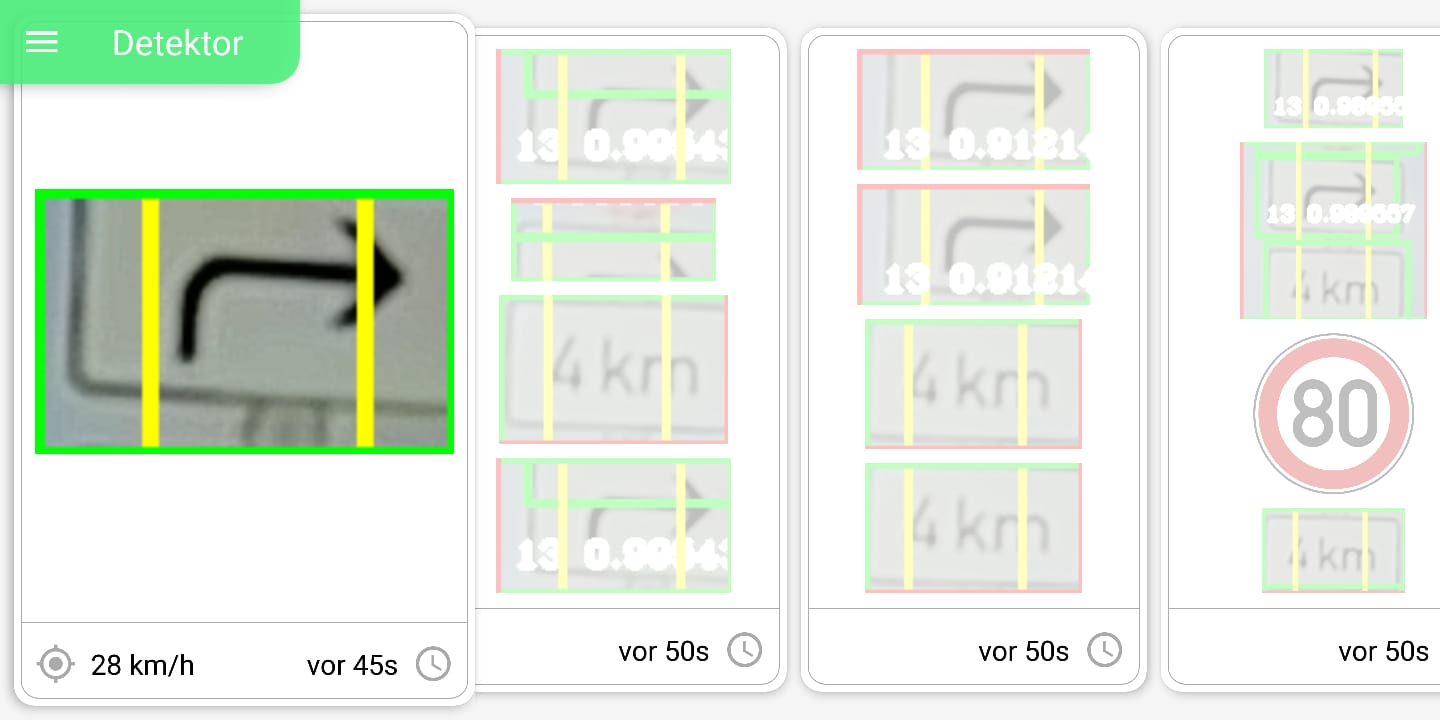
\includegraphics[width=0.9\linewidth]{Reviewdokument/Grafiken/mehrfachdetektion.jpeg}
\caption{Beispielhafte Mehrfachdetektion}
\label{fig:mehrfachdetektion}
\end{figure}

\subsection{Gruppierungsfilter}
Um eine bessere, sortierte Anzeige der erkannten \gls{Verkehrszeichenkombination}en gewährleisten zu können, wurde ein weiterer  \gls{Filter} in der \gls{Verkehrszeichen-API} implementiert, welcher alljene Verkehrszeichen, die am selben Mast montiert sind, gruppiert. Dieser Filter ist der letzte \gls{Filter} in der \glslink{Pipe}{Pipeline}. Das Vorgehen zur Gruppierung der erkannten Verkehrszeichen verläuft wie folgt:
\begin{enumerate}
    \item Erstelle für das erste erkannte Verkehrszeichen ein neues Objekt von Typ \\ \texttt{DetectedSignCombination}, welches eine \gls{Verkehrszeichenkombination} darstellt.
    
    \item Errechne aus der linken und rechten X-Koordinate der Box dieses Verkehrszeichens die Mitte. Dies ist in etwa die Position des Masts, an dem es montiert ist.
    
    \item Betrachte das nächste erkannte Verkehrszeichen und berechne die Position des Masts analog zu 2)
    
    \item Iteriere über alle bisher erstellten Verkehrszeichenkombinationen und vergleiche jeweils die erwartete Position der Masten von Schild und Kombination.
    
    \begin{itemize}
        \item Falls diese etwa gleich sind\footnote{Anm.: das heißt, dass sich die gelben Bereiche aus \cref{fig:mehrfachdetektion} überlappen}, wird das Verkehrszeichen der Kombination hinzugefügt und die erwartete Mitte (die erwartete Position des Masts) aus dem Durchschnitt der Mitten aller erkannten einzelnen Verkehrszeichen der \gls{Verkehrszeichenkombination} neu berechnet
           
        \item Falls der vorhergehende Fall für keine Verkehrszeichenkombination eingetreten ist, erstelle ein neues Objekt vom Typ \\ \texttt{DetectedSignCombination} für das erkannnte Verkehrszeichen.   
    \end{itemize}
    
    \item Wiederhole diesen Vorgang für alle erkannten Verkehrszeichen
\end{enumerate}
\smallskip

\section{Änderungen an den Neuronalen Netzwerken}
\subsection{Implementierung eines neuen Klassifikators}
\label{subsec:neuer-klassifikator}
Aufgrund der sehr schlechten Erkennungsrate des alten \glslink{Klassifikation}{Klassifikators}  wurde ein Wechsel auf einen neuen \glslink{Klassifikation}{Klassifikator} vollzogen. 

Dabei wurde \gls{Keras} als Front End mit TensorFlow als Back End benutzt und MobileNetV2 soweit implementiert, dass es sich trainieren lies. Vortrainierte Gewichte konnten dabei nicht verwendet werden, weil für die verwendete Situation schlichtweg keine existierten. Die Batch-Größe wurde von vorher 96 auf nun 128 erhöht. Beim Training wurde nicht mehr auf das TensorFlow-Format zurückgegriffen, sondern es wurden direkt die Bildateien verwendet, in dem Zuge wurde auf die \gls{Sample}s auch eine leichte, zufällige Translation, Rotation und Vergrößerung angewendet, damit das \glslink{Neuronales Netzwerk}{Neuronale Netzwerk} beim Training eine größere Vielfalt der \gls{Sample}s bekam.\\

Das Ergebnis dieser Neuimplementierung des \glslink{Klassifikation}{Klassifikators} ist die in \cref{fig:konfusionsmatrix} abgebildete Konfusionsmatrix. Diese zeigt, mit welcher Wahrscheinlichkeit sich das \gls{Klassifikation}snetzwerk für eine bestimme Klasse bei gegebener Eingabe entscheidet. Die einzelnen Elemente stellen die Wahrscheinlichkeit dar, mit der sich der \glslink{Klassifikation}{Klassifikator} für die Klasse auf der Abszissenachse entscheiden würde, wenn die tatsächliche Eingabe die Klasse auf der Ordinatenachse ist. Die Summe aller Elemente einer Zeile muss also für jede Zeile 1 ergeben.\\
Je stärker die Hauptdiagonale besetzt ist, und je weniger die Ergebnisse streuen, desto besser ist der \glslink{Klassifikation}{Klassifikator}. Ein perfekter \glslink{Klassifikation}{Klassifikator} besäße die Einheitsmatrix als Konfusionsmatrix, würde sich also mit der Wahrscheinlichkeit 1 für die richtige Klasse entscheiden und mit der Wahrscheinlichkeit 0 für eine der falschen Klassen entscheiden. Um verschiedene \glslink{Klassifikation}{Klassifikatoren} nach ihrer Erkennungsleistung bewerten zu können, summiert man die Elemente der Haupdiagonalen auf; bei 47 verschiedenen Klassen wäre die bestmögliche Bewertung für einen \glslink{Klassifikation}{Klassifikator} also 47. Ein hoher Wert heißt hier, dass sich der \glslink{Klassifikation}{Klassifikator} mit hoher Wahrscheinlichkeit für die richtigen Klassen entscheidet. Die Bewertung des verwendeten \glslink{Klassifikation}{Klassifikators} nach diesem Schema ist 41, was bereits einen relativ hohen Wert darstellt und eine starke Verbesserung vom alten \glslink{Klassifikation}{Klassifikators} ist, welcher lediglich den Wert 25 besaß.\\
Ist man an der \textit{Accuracy} des \glslink{Klassifikation}{Klassifikators} interessiert, d.h. mit welcher Wahrscheinlichkeit im Mittel (falls als Klassen gleichwahrscheinlich auftreten) eine richtige \gls{Klassifikation} zu erwarten ist, so dividiert man die Summe über der Hauptdiagonalen durch die Anzahl an Klassen. Für den alten \glslink{Klassifikation}{Klassifikators} beträgt die Accuracy gerade einmal 53,3\%, wohingegen der neue \glslink{Klassifikation}{Klassifikators} eine Accuracy von 87,2\% besitzt.\\
Die Annahme, dass alle Klassen gleichwahrscheinlich auftreten, ist allerdings meistens nicht richtig. So tritt beispielsweise \gls{VZ} 274 (zulässige Höchstgeschwindigkeit) verglichen mit anderen Klassen deutlich häufiger auf, und genau dort streut die Konfusionsmatrix des alten \glslink{Klassifikation}{Klassifikators} auch sehr stark, was hier besonders fatal ist. Tatsächlich ist der Unterschied zwischen dem alten und dem neuen \glslink{Klassifikation}{Klassifikators} also noch drastischer. Unter Berücksichtigung der Auftrittswahrscheinlichkeit der einzelnen Klassen besitzt der neue \glslink{Klassifikation}{Klassifikator} eine Accuracy von 98\%.\\

Für den \glslink{Klassifikation}{Klassifikator} wurde der eigens gelabelte Datensatz (sh. \cref{sec:eigens_gelabelte_verkehrszeichen}) in Verbindung mit GTSRB verwendet. Dabei wurden die nun vorhandenen Daten im Verhältnis 9:1 geteilt; es wurden die ersten 10\% jeder Klasse als Testdaten reserviert und der Rest als Trainingsdaten verwendet. Anhand ersterer wurden die Konfusionsmatrizen erstellt und daraus der beste \glslink{Klassifikation}{Klassifikator} ausgewählt.

\begin{figure}[H]
\centering
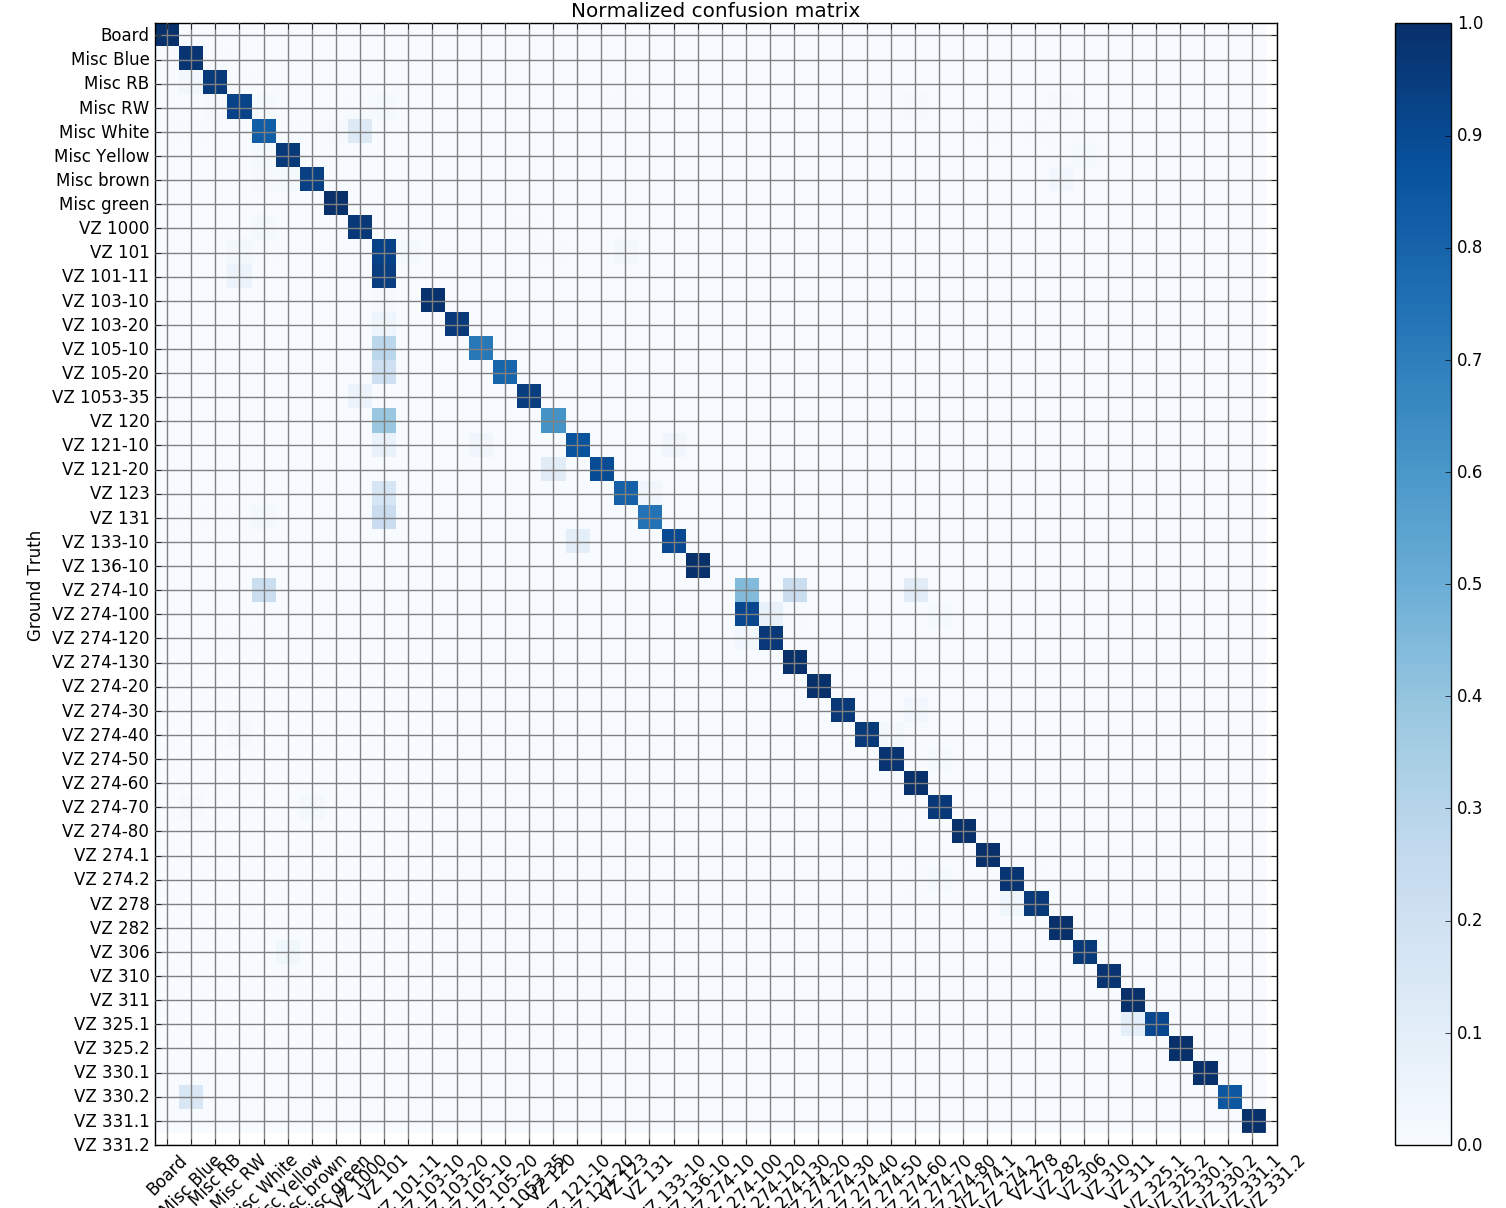
\includegraphics[width=1\linewidth]{Reviewdokument/Grafiken/konfusionsmatrix.png}
\caption{Normierte Konfusionsmatrix des neuen Klassifikators, $\sum\limits_{i=0}^{N-1}a_{i,i} \approx 41$}
\label{fig:konfusionsmatrix}
\end{figure}

\subsubsection*{Unregelmäßigkeiten in der Konfusionsmatrix}
\begin{description}
    \item[(\gls{VZ} 101-11, \gls{VZ} 101)] \gls{VZ} 101-11 (Gefahrenzeichen Fußgängerüberweg) befindet sich kaum in den Trainingsdaten, also würde sich der Klassifkator bei Eingabe dieser Klasse eher für \gls{VZ} 101 entscheiden, was dem generischen Gefahrenzeichen entspricht.\\
    Dass sich der \glslink{Klassifikation}{Klassifikator} fast immer für \gls{VZ} 101 entscheidet, kann u.A. daran liegen, dass \gls{VZ} 101 verglichen mit \gls{VZ} 101-11 deutlich überrepräsentiert ist. Inkonsistentes \glslink{Label}{Labeling} könnte ebenfalls dazu beitragen.
    \item[(\gls{VZ} 274-10, \gls{VZ} 274-100)] Da der Datensatz nur sehr wenige \gls{Sample}s für \gls{VZ} 274-10 (zul. Höchstgeschw. 10 km/h) enthält, wird der \glslink{Klassifikation}{Klassifikator} sich wahrscheinlich eher für die Klasse \glqq{}Sonstige rot/weiß\grqq{} oder für ein \gls{VZ} 274 mit einer anderen Zahl entscheiden.
\end{description}
\smallskip

Trotz dieser beiden Unregelmäßigkeiten ist die Konfusionsmatrix dennoch relativ gut. Die Wahrscheinlichkeit für eine korrekte \gls{Klassifikation} ist bei den meisten Klassen, insbesondere bei allen geschwindigkeitsregulierenden Verkehrszeichen (bis auf \gls{VZ} 274-10) sehr hoch. \\\\
Im Vergleich dazu zeigt \cref{fig:konfusionsmatrix_alt} den alten \glslink{Klassifikation}{Klassifikator}.

\begin{figure}[H]
\centering
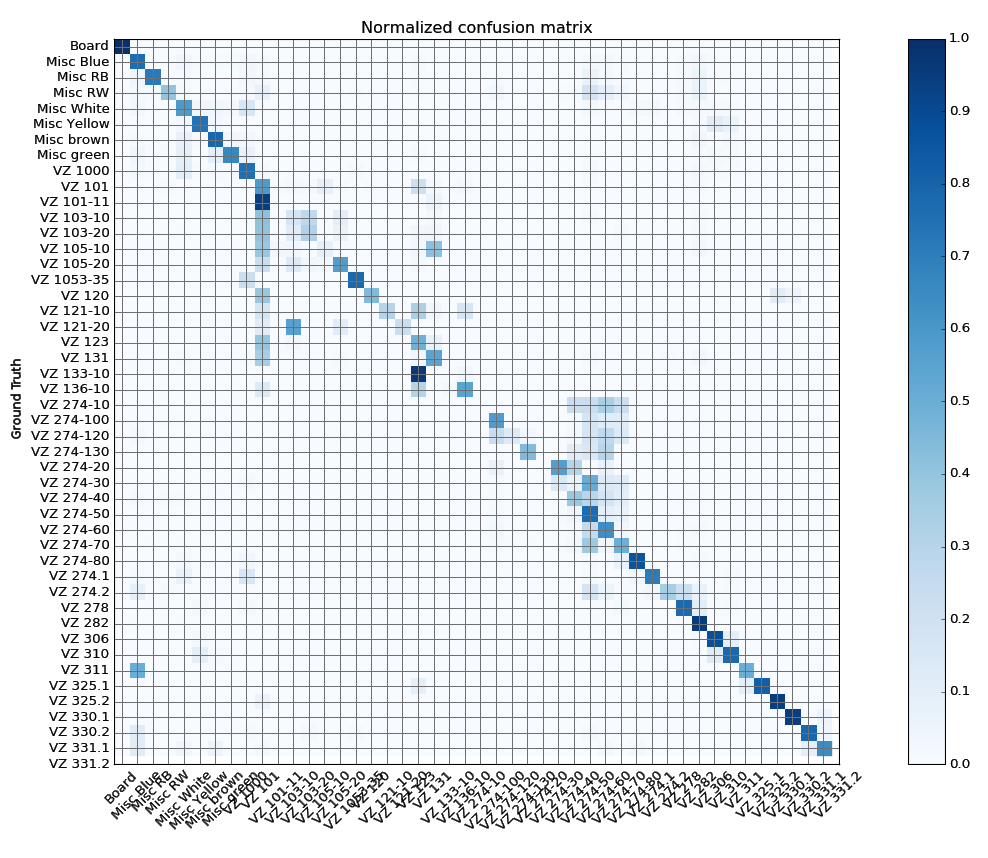
\includegraphics[width=1\linewidth]{Reviewdokument/Grafiken/Konfusionsmatrix_alt.png}
\caption{Normierte Konfusionsmatrix des alten Klassifikators, $\sum\limits_{i=0}^{N-1}a_{i,i} \approx 25$}
\label{fig:konfusionsmatrix_alt}
\end{figure}

\chapter{Bug-Review}

\section{Bugs in der App}

\subsection{Verursachung von Scroll-Artefakten}
Wenn der \gls{Nutzer} in dem Detektionsmenü der \gls{App} zu schnell in eine Richtung scrollt, traten dabei Artefakte auf. Das heißt, dass in den angezeigten Karten teilweise Verkehrszeichen falsch skaliert oder sogar in der falschen Kombination auftraten. Dies lag wahrscheinlich daran, dass diese Karten in einem \texttt{RecyclerView}\footnote{\link{https://developer.android.com/guide/topics/ui/layout/recyclerview}, 26.06.2018} organisiert werden, welcher nur die aktuell sichtbaren Karten anzeigt und die nicht-sichtbaren Karten erst lädt, wenn man auf diese hinscrollt. Natürlich benötigt dies eine gewisse - wenn auch sehr geringe - Ladezeit, was vermutlich dazu führte, dass bei zu schnellem Scrollen die Karten falsch aktualisiert wurden.\\
Einige Tage später wurde erfolglos versucht, diesen Bug zu reproduzieren. Da er nicht reproduziert werden konnte, wurde er daraufhin ignoriert. Es besteht die Möglichkeit, dass er infolge anderer Änderungen bereits gelöst wurde.

\begin{description}

    \item[Erkannt am:] 06.06.2018
    
    \item[Aktueller Status:] Konnte nicht reproduziert werden und wurde daraufhin ignoriert.
    
    \item[Zukünftiges Risiko:] Es besteht ein Restrisiko, dass der Bug noch immer vorhanden ist. Da er zur Zeit des zweiten Tests allerdings als nicht reproduzierbar war und die Situation während der Fahrt aufgrund des Verbotes der Bedienung nicht auftreten sollte, besaß dessen Korrektur eine relativ geringe Priorität.
    
\end{description}
\smallskip

\subsection{Drücken des Zurück-Buttons aktualisierte den Titel nicht}
Jedes Fragment besitzt einen Titel, welcher gut sichtbar in der oberen linken Bildschirmecke angezeigt wird. Es gibt die Möglichkeit für den \gls{Nutzer}, durch Drücken des Zurück-Buttons (das nach links zeigende Dreieck am Bildschirmrand) in die zuvor aktiven Fragmente zu navigieren. Dabei wurde allerdings dieser Titel in der oberen linken Ecke nicht aktualisiert.\\
Dieser Bug wurde dadurch korrigiert, dass die Methode \texttt{onBackPressed()} des Android-Frameworks dahingehend überschrieben wurde, sodass der Titel des aufgerufenen Fragmentes abgefragt und entsprechend angezeigt wird.

\begin{description}

    \item[Erkannt am:] 06.06.2018
    
    \item[Aktueller Status:] Seit dem 21.06.2018 korrigiert.
    
    \item[Zukünftiges Risiko:] Stellt kein weiteres Risiko dar.
    
\end{description}
\smallskip

\subsection{Zu häufiges Drücken des Zurück-Buttons führe dazu, dass nichts mehr angezeigt wurde}
Wenn der \gls{Nutzer} den Zurück-Button öfter drückt, als er zuvor Fragmente geöffnet hatte, führte dies dazu, dass gar kein Fragment mehr angezeigt wurde. Dass man mit dem Zurück-Button durch die Fragmente zurücknavigieren kann, wird dadurch ermöglicht, dass man beim Anzeigen eines neuen Fragmentes ein neues Element in den sogenannten \glqq{}BackStack\grqq{} pushed. Wenn man das allerdings auch für das erste angezeigte Fragment macht, dann kann das auch mit entfernt werden und es bleibt keines mehr übrig, was dazu führte, dass die \gls{App} kein Fragment mehr anzeigte.\\
Dieser Bug wurde dadurch korrigiert, dass nun beim Öffnen des ersten Fragmentes ein Flag gesetzt wird. Erst ab diesem Setzen wird beim Öffnen von Fragmenten der BackStack verwendet. Dadurch bleibt das erste Fragment außen vor und ist nicht mehr durch den Zurück-Button entfernbar. Stattdessen wird nun, wenn der \gls{Nutzer} in diesem Fragment den Zurück-Button drückt, die App beendet.

\begin{description}

    \item[Erkannt am:] 06.06.2018
    
    \item[Aktueller Status:] Seit dem 21.06.2018 korrigiert.
    
    \item[Zukünftiges Risiko:] Stellt kein weiteres Risiko dar.
    
\end{description}
\smallskip

\subsection{Zurvor erkannte Verkehrszeichen verschwinden aus der Historie}
Wenn das Detektor-Fragment vorher schon eine Weile gelaufen ist, und der \gls{Nutzer} dann durch einige Menüs hin und her navigiert und zum Detektor zurückkehrt, wurden (vermeintlich zufällig) einige Einträge der Historie gelöscht. Dies lag daran, dass die Historie selbst in der Laufzeit der \gls{App} gespeichert wurde, eine zugehörige Zählervariable \texttt{FrameID} allerdings nur in der Laufzeit des Detektor-Fragmentes, welche damit beim Wechseln des Fragmentes zurückgesetzt wird.
Der Algorithmus zum Zusammenfassen von Verkehrszeichenkombinationen benutzt allerdings die \texttt{FrameID} um herauszufinden, mit welchen Kombinationen eine Zusammenfassung sinnvoll wäre. Nun passierte es, dass die zurückgesetzte Zählervariable wieder alte erkannte Kombinationen als aktuell markierte und diese somit fälschlicherweise aktualisiert werden konnten. Da beim Aktualisieren einer alten Kombination diese aus der Historie entfernt wird, um die neuere vorne anzufügen, verschwanden sie einfach aus der Anzeige.\\
Dieser Bug wurde dadurch korrigiert, dass beim erneuten Wechsel zum Detektorfragment die aktuelle \texttt{FrameID} nun abgefragt wird und entsprechend die Zählervariable nicht mehr bei 0 anfängt zu zählen.

\begin{description}

    \item[Erkannt am:] 25.06.2018
    
    \item[Aktueller Status:] Seit dem 25.06.2018 korrigiert.
    
    \item[Zukünftiges Risiko:] Stellt kein weiteres Risiko dar.
    
\end{description}
\smallskip

\subsection{Fehlerhafte Behandlung der Skalierung von Bildausschnitten}
Die \gls{App} zeigt manche Verkehrszeichen nicht als Vektorgrafiken, sondern als Ausschnite aus dem aufgenommenen Bild an. Dies ist beispielsweise bei Zusatzzeichen der Fall, wo eine korrekte \gls{Klassifikation} schwierig ist. Wenn Bildausschnitte zusammen mit den Grafiken angezeigt werden, müssen die Bildausschnitte in der Skalierung extra behandelt werden. Wenn eine Karte aktualisiert wird (z.B. wenn dieselbe \gls{Verkehrszeichenkombination} noch einmal erkannt wurde), werden auch die Grafiken aktualisiert, wobei es passieren konnte, dass bezüglich der Skalierung nicht extra behandelte Bildausschnitte in eine andere Karte kommen konnten und dort viel zu klein dargestellt wurden.\\
Dieser Bug wurde dadurch korrigiert, dass die Sonderbehandlung der Bildausschnitte bei Notwendigkeit nun nachgeholt wird, wenn \gls{Verkehrszeichenkombination}en beim Aktualisieren zusammengefügt werden.

\begin{description}

    \item[Erkannt am:] 25.06.2018
    
    \item[Aktueller Status:] Seit dem 25.06.2018 korrigiert.
    
    \item[Zukünftiges Risiko:] Stellt kein weiteres Risiko dar.
    
\end{description}
\smallskip

\subsection{Aktuell angezeigtes Verkehrszeichen wurde nicht aktualisiert}
Bei der Darstellung der \gls{Verkehrszeichenkombination}en in den einzelnen Karten wurde versucht, eine Optimiertung vorzunehmen, welche darin bestand, dass die Verkehrszeichen in den \texttt{ImageView}s nur dann neu geladen werden sollten, wenn sie sich auch tatsächlich änderten. Diese \glqq{}Optimierung\grqq{} führte allerdings aus einem noch nicht ausgemachten Grund dazu, dass nach Hin- und Herwechseln vom Detektor-Fragment die aktuelle \gls{Verkehrszeichenkombination} nicht mehr richtig angezeigt wurde. Entweder war die Karte der aktuellen \gls{Verkehrszeichenkombination} komplett leer oder es wurde eine alte \gls{Verkehrszeichenkombination} angezeigt.\\
Da der wirkliche Grund für diesen Bug noch nicht ausgemacht wurde, wurde er dadurch korrigiert, dass diese \glqq{}Optimierung\grqq{} für die Karte der aktuellen \gls{Verkehrszeichenkombination} rückgängig gemacht wurde. Für die Historie wurde sie allerdings beibehalten, da dort keine solche Probleme festgestellt wurden.

\begin{description}

    \item[Erkannt am:] 25.06.2018
    
    \item[Aktueller Status:] Seit dem 25.06.2018 korrigiert.
    
    \item[Zukünftiges Risiko:] Es besteht ein geringes Risiko, dass in der Historie Fehler auftreten können, wie sie bei der aktuellen \gls{Verkehrszeichenkombination} beobachtet wurden.
    
\end{description}
\smallskip

\subsection{Historie \glqq{}springt\grqq{} manchmal hin und her}
Gelegentlich springt die Historie unerwartet hin und her. Dies tritt vor allem dann auf, wenn in kurzer Zeit relativ viele Verkehrszeichen in die Historie hinzugefügt werden. Der Bug wurde noch nicht genauer untersucht.

\begin{description}

    \item[Erkannt am:] 25.06.2018
    
    \item[Aktueller Status:] Noch vorhanden.
    
    \item[Zukünftiges Risiko:] Der Bug beeinflusst als kleiner Grafikfehler die Benutzbarkeit nicht in signifikantem Maße.
    
\end{description}
\smallskip

\subsection{Bildrotation unter Umständen fehlerhaft}
Je nach Orientierung des Kamerasensor und Orientierung des Gerätes konnte es passieren, dass das aufgenommene Kamerabild auf den Kopf gestellt war, wodurch natürlich keine sinnvolle \gls{Detektion} oder \gls{Klassifikation} mehr möglich war.\\
Dies wurde dadurch korrigiert, dass nun die Orientierung des Sensors und die Orientierung des Gerätes vorher abgefragt werden, und das aufgenommene Bild falls nötig um 180° gedreht wird.

\begin{description}

    \item[Erkannt am:] 29.06.2018
    
    \item[Aktueller Status:] Seit dem 30.06.2018 korrigiert.
    
    \item[Zukünftiges Risiko:] Stellt kein weiteres Risiko dar.
    
\end{description}
\smallskip

\subsection{Angezeigte Geschwindigkeit zu niedrig}
Um Ausreißer zu vermeiden, wurde eine Änderung an der Geschwindigkeitsanzeige vorgenommen - der Algorithmus dazu ist in \cref{subsec:verbesserung-geschwindigkeitsermittlung} beschrieben. Bei der ersten Testfahrt nach dieser Verbesserung fiel auf, dass der angezeigte Wert stets um etwa 20\% nach unten vom Tachometer abwich. Dies lag einfach daran, dass bei der Mittelung aus dem Ringspeicher der falsche Divisor gewählt wurde. Bei fünf GPS-Positionen im Ringspeicher besitzt man nämlich nicht fünf Geschwindigkeitswerte, sondern nur vier, weil die Abschnitte zwischen den Positionen, nicht die Positionen selbst gezählt werden müssen.\\
Dieser Fehler wurde dadurch korrigiert, dass nun der korrekte Divisor (im Beispiel 4 anstatt 5) gewählt wurde.

\begin{description}

    \item[Erkannt am:] 29.06.2018
    
    \item[Aktueller Status:] Seit dem 30.06.2018 korrigiert.
    
    \item[Zukünftiges Risiko:] Stellt kein weiteres Risiko dar.
    
\end{description}
\smallskip

\newpage
\section{Bugs im Back End}

\subsection{Unzureichende Erkennungsrate des Klassifikators} 
Beim Training des \glslink{Klassifikation}{Klassifikators} fiel auf, dass die Erkennungsrate für das vergleichsweise einfache Problem der Verkehrszeichen-\gls{Klassifikation} klassenübergreifend zu niedrig war. So gab es beispielsweise die Klasse \gls{VZ} 274-120 (zul. Höchstgeschw. 120 km/h), welche auf den Validierungsdaten gerade einmal zu 10\% erkannt wurde, da der \glslink{Klassifikation}{Klassifikator} ihm ähnlich aussehende Klassen zugeordet hat.\\
Es gab mehrere Versuche dieses Problem zu beheben. Als erstes wurden verschiedenste Klassengewichte getestet, was das Problem allerdings nicht behoben hat. Danach wurden weniger \gls{Sample}s derer Klassen zum Training benutzt, welche weitaus mehr \gls{Sample}s hatten als andere Klassen. Allerdings führte dies ebenfalls zu keiner Verbesserung. Weiterhin wurde versucht, den \glslink{Klassifikation}{Klassifikator} nur auf die Verkehrszeichen, welche unter die Klassen \gls{VZ} 274 fallen, zu trainieren. Dies führte allerdings auch zu keiner Verbesserung. In diesem Durchgang hat das \glslink{Neuronales Netzwerk}{Netzwerk} fast ausschließlich die Klasse \gls{VZ} 274-70 gelernt und alle anderen Verkehrszeichen auch dementsprechend als \gls{VZ} 274-70 klassifiziert. Das gleiche Training wurde noch einmal unter der Beachtung, dass alle Klassen gleich viele \glslink{Sample}{Samples} enthalten, durchgeführt. Das Resultat war deutlich besser als zu allen Versuchen davor, allerdings immer noch deutlich schlechter als erwartet. Des Weiteren wurden verschiedene Optimierungsverfahren, vortrainierte Modelle, Lernraten und Klassengewichte getestet, was jedoch ebenfalls nicht zur Verbesserung beigetragen hat.\\
Nach vielen erfolglosen Versuchen wurde das Netzwerk, sowie das Training von Grund auf neu in \gls{Keras} implementiert. Nach dem Training mit \gls{Keras} war die Erkennungsrate deutlich besser, was die Konfusionsmatrix \cref{fig:konfusionsmatrix} unter \cref{subsec:neuer-klassifikator} zeigt. \\
Da zum Training in \gls{TensorFlow Mobile} die Trainingsskripte von TensorFlow-Slim\footnote{\link{https://github.com/tensorflow/models/tree/master/research/slim}, 01.07.2018} benutzt wurden, ist anzunehmen, dass diese Fehler enthalten. Es ist nicht gelungen, den genauen Fehler ausfindig zu machen, allerdings war es möglich ihn durch die Implementierung in \gls{Keras} zu umgehen.

\begin{description}

    \item[Erkannt am:] 26.06.2018
    
    \item[Aktueller Status:] Seit dem 26.06.2018 korrigiert. 
    
    \item[Zukünftiges Risiko:] Stellt kein weiteres Risiko dar. 
    
\end{description}
\smallskip

\chapter{Nachweis der Abnahmekriterien}
Im Folgenden sei die Erfüllung bzw. Nichterfüllung der im Pflichtenheft in Abschnitt 8 (S.14ff) beschrieben Abnahmekriterien und Testfälle beschrieben.\\

\section{Funktionale Anforderungen}

\begin{description}

    \item[A001: Testfahrt]~\\ In der 45-minütigen Testfahrt der im Pflichtenheft spezifizierten Teststrecke entlang wurden lediglich vier Verkehrszeichen nicht erkannt - zweimal \gls{VZ} 1001-31 (auf ... km), einmal \gls{VZ} 274-70 (zul. Höchstgeschw. 70 km/h) und einmal \gls{VZ} 274-80 (zul. Höchstgeschw. 80 km/h). Insbesondere die zuvor als risikoreich eingeschätzten \gls{VZ} 310 u. 311 (Ortstafel) und \gls{VZ} 330 (Autobahn) wurden fast immer korrekt erkannt. Eine \gls{Verkehrszeichenkombination} bestehend aus \gls{VZ} 274-30 (zul. Höchstgeschw. 30 km/h) und \gls{VZ} 103 (gefährliche Rechtskurve) konnte nicht erkannt werden, da es von einem Baum verdeckt wurde, woraufhin die Betriebsbedingungen nicht mehr gegeben waren.\\
    Bei etwa 60 befahrenen Verkehrszeichen liegt die Fehlerrate dabei also bei unter 10\%.\\
    Es wurden einige Male fälschlicherweise Werbeplakate als Ortstafeln erkannt. Dies lag daran, dass auf diesen Werbeplakaten eine Ortstafel abgedruckt war. Diesen Randfall auszusortieren wäre, wenn überhaupt, nur mit einem viel umfangereicherem Datensatz möglich.
    
    \item[A002: Einbindbarkeit der \gls{Filterverwaltungs-Bibliothek}]~\\ Für die \gls{Verkehrszeichen-API} wurden exemplarisch vier Filter angelegt, durch die die \gls{Filterverwaltungs-Bibliothek} eingebunden wird. Wie im Pflichtenheft beschrieben liegt die Beweislast für diesen Testfall im Allgemeinen beim Kunden.
    
    \item[A004: Einstellung der Historie]~\\ Wurde durch Einstellen der gewünschen Anzahl und anschließendes Abzählen der Einträge in der Historie verifiziert.
    
    \item[A005: Geschwindigkeitsanzeige]~\\ Bei eingeschalteter Geschwindigkeitserkennung (sh. A006) wurde diese Anforderung durch Vergleich der angezeigen Geschwindigkeit unter dem aktuellen Verkehrszeichen mit der angezeigten Geschwindigkeit einer Navigationsapp verifiziert. Beim Vergleich mit dem Fahrzeugtachometer ergeben sich erwartungsgemäß Abweichungen nach unten, da dieser bekanntlicherweiser etwas \glqq{}nachgeht\grqq{}.

    \item[A006: Einstellung der Geschwindigkeitsanzeige]~\\ Wenn der \gls{Nutzer} keine Geschwindigkeitsanzeige wünscht, wird der GPS-Sensor auch nicht abgefragt, wodurch es für die \gls{App} keine Möglichkeit gibt, die Geschwindigkeit verlässlich zu bestimmen. Wenn die Geschwindigkeitsanzeige abgeschaltet ist, wird stattdessen unter dem aktuellen Verkehrszeichen eine Tilde angezeigt.
    
    \item[A007: Warnhinweis]~\\ Kann bei jedem Start der \gls{App} verifiziert werden. Dieser Haftungsausschluss muss bestätigt werden, um fortfahren zu können; er befindet sich ferner auch in einem Untermenü in der \gls{App} und auch im Benutzerhandbuch.
    
    \item[A008: Kalibrierung]~\\ Das Kalibrierungsmenü wird beim Start der App nach Bestätigung des Haftungsausschlusses angezeigt. Der \gls{Nutzer} hat die Möglichkeit, dieses Menü auch später nocheinmal aufzurufen, falls er bemerkt, dass die Smartphonehalterung schief hängt. Als Schwellwert wurde eine \glslink{Drehachsen}{Neigung und Drehung} von jeweils 5° festgelegt - eine größere Abweichung von der waagerechten Nulllage gilt nicht mehr als kalibriert. Alle sonstigen Kalibrierungen (insb. Kamerafokus, Brennweite, etc.) werden automatisch von der \gls{App} festgelegt.
    
    \item[A009: Überlagerung über andere Apps]~\\ Die zugehörige Anforderung wurde nicht umgesetzt, der Testfall wurde also nicht erfüllt. Siehe \cref{nichtumgesetzte-anforderungen}. 
    
    \item[A010: Abgleich mit Kartendaten]~\\ Die zugehörige Anforderung wurde nicht umgesetzt, der Testfall wurde also nicht erfüllt. Siehe \cref{nichtumgesetzte-anforderungen}. 
    
\end{description}
\smallskip

\section{Nichtfunktionale Anforderungen}

\begin{description}

    \item[A003: Parallelität der \gls{Filterverwaltungs-Bibliothek}]~\\ Für die \gls{Verkehrszeichen-API} wurden exemplarisch vier Filter angelegt, durch die die \gls{Filterverwaltungs-Bibliothek} eingebunden wird. Wie im Pflichtenheft beschrieben liegt die Beweislast für diesen Testfall im Allgemeinen beim Kunden.

    \item[A011: Erkennung in 1 s]~\\ Wurde anhand einer Aufnahme der Testfahrt auszugsweise verifiziert.
    
    \item[A012: Funktion ohne Internet]~\\ Die \gls{App} fragt niemals eine Internetverbindung ab. Im gesamten Quellcode gibt es keine einzige Anfrage auf Internetverbindung und auch im Android Manifest\footnote{\link{https://developer.android.com/guide/topics/manifest/manifest-intro}, 25.06.2018} wird die dafür notwendige Berechtigung nicht angefordert - würde die \gls{App} also versuchen, auf das Internet zuzugreifen, würde das Betriebssystem diese augenblicklich mit einer Exception beenden.
    
    \item[A013: Modularität des Back Ends]~\\ Für die \gls{Verkehrszeichen-API} wurden exemplarisch vier Filter angelegt, durch welche die \gls{Filterverwaltungs-Bibliothek} eingebunden wird. Wie im Pflichtenheft beschrieben liegt die Beweislast für diesen Testfall im Allgemeinen beim Kunden.
    
\end{description}

% -----------------------------------------

\part{Rückblickende Betrachtung}

\chapter{Bewertung des Vorgehensmodelles}

\section{Ursprüngliches Vorgehensmodell}
Die Wahl des Vorgehensmodelles für das Softwareprojekt wurde durch die Auftraggeber nicht festgelegt. Die Wahl fiel auf das \emph{agile Vorgehensmodell}, da dieses aufgrund der Flexibilität am ehesten den Anforderungen des Projektes gerecht wurde: aufgrund der Unvorhersehbarkeit des Erfolges gewählter Strategien und Lösungsansätze musste dynamisch auf neue Erkenntnisse und ggf. Fehlschläge reagiert werden können und das Vorgehen dementsprechend angepasst werden.\\
In einem so stark umforschten Themengebiet wie dem  \gls{Deep Learning}, welches viel Austesten benötigt, ist es vorteilhaft, nicht an ein zu Beginn festgelegtes Schema gebunden zu sein und stets notwendige Änderungen vornehmen zu können.
Diese Vorteile sind auch teils bei Unified Process gegeben, allerdings war die noch freiere Handhabung im agilen Vorgehen adäquater für die Projektgruppe.\\

\subsection{Anpassungen}
Als Grundkonzept des agilen Vorgehensmodelles galten die Bestimmungen, welche auf der Website des Fachgebietes für System- und Software-Engineering\footlink{https://www.tu-ilmenau.de/sse/lehre/softwareprojekt/projektablauf/}{29.04.2018} vorgeschrieben sind. Davon abweichend wurde die Gruppe in Teams unterteilt, da aufgrund des Umfangs und Einarbeitungsaufwandes für die Einzelthemen es im Rahmen des Softwareprojektes schlichtweg nicht möglich war, dass jedes Gruppenmitglied alle Teilgebiete des Projekts vollständig beherrscht.\\

\section{Bewertung}
Die Vorteile des agilen Vorgehensmodell und der Grund, weshalb es ursprünglich gewählt wurde, war, um dynamisch auf unerwartete Erfolge und Fehlschläge reagieren zu können. Größtenteils war es allerdings nicht notwendig, von diesen Vorteilen Gebrauch zu machen. Es gab drei Rückschläge im Projekt - die grobe Fehlabschätzung des Zeitaufwandes für die \gls{Sample}s, die Inkompatibilität von \gls{TensorFlow Lite} mit dem Single Shot Detector sowie die Probleme des Trainings des \glslink{Klassifikation}{Klassifikators}. Diese hätten jedoch auch mit anderen Vorgehensmodellen adäquat gehandhabt werden können.\\
Rückblickend betrachtet wurden die ursprünglichen Vorteile des agilen Vorgehensmodelles nicht benötigt, was aber keineswegs bedeutet, dass die Entscheidung dafür die falsche war. \emph{Wäre} es zu sehr großen Fehlschlägen gekommen, \emph{hätte} das agile Vorgehensmodell noch die besten Chancen gelassen.\\

Aufgrund der Strukturierung des Softwareprojektes ist ein \glqq{}richtiges\grqq{} agiles Vorgehensmodell allerdings nur mit Einschränkungen möglich. Die Einteilung des Projektes in drei Phasen (Entwurf, Implementierung, Test) und die entsprechend geforderten Reviewdokumente hatten zur Folge, dass in den einzelnen Iterationen der Fokus doch sehr stark auf den Inhalt der jeweiligen Dokumente gelegt wurde. Unser Projektplan (sh. Reviewdokument Phase II) spiegelt dies auch wieder - in der ersten Iteration wurde hauptsächlich Entwurfsdokumentation angefertigt, in der zweiten Iteration implementiert und in der dritten Iteration getestet. Von daher ist es durchaus fragwürdig, ob tatsächlich das agile Vorgehensmodell gewählt wurde. Wahrscheinlich entsprach das durchgeführte Vorgehen eher einer Mischung aus dem agilen Vorgehenesmodell und dem Rational Unified Process. Es gab durchaus eine starke Diskrepanz zwischen den Fokussen der einzelnen Phasen, aber gleichzeitig wurde bereits zu Ende der ersten Iteration jeweils ein Prototyp zur \gls{App} und zu den \glslink{Neuronales Netzwerk}{Neuronalen Netzen} fertiggestellt, welcher in den folgenden Iterationen weiterentwickelt wurde, was wiederum eine Eigenschaft des agilen Vorgehens ist.\\
Der Leitwert des agilen Vorgehensmodelles, keine Überstunden zu arbeiten, wurde definitiv \emph{nicht} eingehalten. Dies war allerdings zwingend notwendig, um einen Erfolg des Projekts sicherstellen zu können.\\

\chapter{Bewertung des Projekterfolges}% ich denke, in dem Abschnitt können wir auch mal von "wir" anstatt von "man" sprechen

Wir sehen das Projekt als Erfolg an. Lediglich einige, in \cref{nichtumgesetzte-anforderungen} beschriebene, Kleinigkeiten konnten keine Beachtung finden. Neben den ursprünglichen geplanten Artefakten des Projektes entstand außerdem ein umfangreicher Datensatz von deutschen Verkehrszeichen, welcher ggf. auch in zukünftigen Projekten verwendet werden kann.\\
Wegen der erfolgreich umgesetzten Modularität und der daraus folgenden Wiederverwendbarkeit ist die Wahrscheinlichkeit groß, dass das einige der Artefakte auch in Zukunft zum Einsatz kommen. Es war für uns als Projektgruppe wichtig, ein Softwareprojekt anzufertigen, welches auch nach Ende des Projektes einen Zweck erfüllen kann.\\

\section{Nicht umgesetzte Anforderungen}
\label{nichtumgesetzte-anforderungen}

\begin{description}

\item[(P4308) Abgleich mit Kartendaten]~\\ Wurde nicht umgesetzt, da es mit großem Aufwand verbunden ist, gleichzeitig aber nur eine geringe Priorität besitzt. Würde man ständig Kartenmaterial extrahieren, würde dies außerdem relativ viel Rechenleistung benötigen, welche eigentlich für die \gls{Detektion} und \gls{Klassifikation} benötigt wird.

\item[(P5003) Überlagerung über andere Apps]~\\ Wurde nur teilweise erfüllt. Die \gls{App} läuft zwar nicht als Dienst (Service)\footnote{\link{https://developer.android.com/guide/components/services}, 15.06.2018} im Hintergrund, sie unterstützt aber den mit Android 7.0 \textit{Nougat} eingeführten Split-Screen-Modus, sodass sie neben einer Navigationsapp laufen kann. Dies funktioniert allerdings nur, sofern diese Navigationsapp ebenfalls den Split-Screen-Modus unterstützt.

\item[(B6005) Warnung bei Geschwindigkeitsunterschreitung]~\\ Falls die aktuelle Situation (z.B. Stau, Glatteis) eine niedrigere Fahrtgeschwindigkeit erfordert als durch \gls{VZ} 275 vorgeschrieben, ist eine Geschwindigkeitsunterschreitung im Sinne der \gls{StVO} §3 nicht nur zulässig, sondern auch vorgeschrieben. Im Allgemeinen kann das \gls{System} solche Situationen nicht erkennen, und würde den Fahrer so verbotenerweise zu einer überhöhten Fahrtgeschwindigkeit motivieren. Deshalb wurde von einer Warnung bei Geschwindigkeitsunterschreitung abgesehen.

\item[(B6006) Akustische Warnung]~\\ Diese Anforderung wurde von vornherein als ein Feature mit geringer Priorität eingestuft und aus Zeitgründen nicht implementiert.

\end{description}

\textbf{Anmerkung}: die Anforderung \textbf{$\llbracket$P4102$\rrbracket$} beschreibt, dass das \gls{System} in der Lage sein soll, Geschwindigkeitsschilder gemäß \gls{StVZO} § 58 als solche zu erkennen und auszusortieren. Das \gls{System} wurde nicht direkt auf diese Funktion hin ausgelegt, aber aufgrund der Wahl des \glslink{Detektion}{Detektors} - insbesondere dessen Auflösung von 300$\times$300 Pixeln - sollte es in der realitätsnahen Anwendung nur in äußerst seltenen Randfällen vorkommen, dass das \gls{System} Schilder in dieser Größe überhaupt erkennen kann. Entsprechend ist die Herausfilterung dieser Schilder nicht zwingenderweise notwendig. Diese Annahme konnte allerdings aufgrund zeitlicher Einschränkungen und dem Fehlen passender Situationen in Testfahrten nicht überprüft werden. \emph{Bei Zutreffen dieser durchaus realistischen Annahme ändert sich an der Funktion des \gls{System}s jedoch nichts}.\\
Ein Algorithmus zur direkten Ausfilterung solcher Fehldetektionen ließe sich nachträglich folgendermaßen umsetzen:\\
Die API ist in der Lage, die überschneidende Fläche detektierter Bereiche zu ermitteln, um Duplikate entfernen zu können. Wenn der Detektor ebenfalls auf die Erkennung von Fahrzeugen trainiert wird, kann dieser Algorithmus dazu erweitert werden, Detektionen innerhalb der zu einem Fahrzeug zugehörig erkannten Bereiche auszufiltern. Diese zusätzliche Absicherung gegen eine solche Art von Fehldetektion wurde aufgrund zeitlicher Einschränkungen allerdings nicht im Rahmen des Softwareprojektes umgesetzt.\\
Von daher kann nicht gesagt werden, ob diese Anforderung erfüllt ist oder nicht. Zwar werden diese Geschwindigkeitsschilder nicht explizit herausgefiltert, aber das \gls{System} ist aufgrund der Umstände prinzipiell dazu in der Lage und für den \gls{Nutzer} ändert sich nichts an der Funktion.\\

\chapter{Ausblick auf zukünftige Projekte}

Im Rahmen dieses Projektes konnten nicht alle Anforderungen umgesetzt werden

\section{Datensatz}
Der erstellte Datensatz (sh. \cref{sec:eigens_gelabelte_verkehrszeichen}) ist deutlich umfangreicher als alle vergleichbaren, für den deutschen Straßenverkehr geltende, Datensätze aus der Literatur. Der größte bisher verfügbare Datensatz war der \textit{German Traffic Sign Detection Benchmark} (GTSDB, \gls{Detektion}) bzw. \textit{German Traffic Sign Recognition Benchmark}\footnote{\link{http://benchmark.ini.rub.de/?section=home\&subsection=news}, 01.07.2018} (GTSRB, \gls{Klassifikation}) der Ruhr-Universität Bochum.\\

\begin{tabu}{|X[l]|X[r]|X[r]|}
    \hline
    ~               & GTSRB/GTSDB               & eigener Datensatz         \\  \hline
    Klassifikation  & $\approx$50.000 Samples   & $\approx$272.000 Samples  \\
    Detektion       & $\approx$900 Samples      & $\approx$50.000 Samples   \\  
    Vielfalt        & 42 Klassen                & 107 Klassen               \\
    \hline
\end{tabu}
\bigskip

Ferner ist der erstellte Datensatz mit dem der Ruhr-Universität Bochum kompatibel, man kann also beim Training bis zu 322.000 \gls{Sample}s für die \gls{Klassifikation} und 50.900 \gls{Sample}s für die \gls{Detektion} verwenden. Der erstellte Datensatz kann in Zukunft veröffentlicht und für andere Projekte verwendet werden. Eine Erweiterung dieses Datensatzes um weitere \gls{Sample}s ist außerdem möglich, um beispielsweise auch sämtliche \gls{VZ} 275 (vorgeschriebene Mindestgeschwindigkeit) erkennen zu können.\\

\section{Tracking}
Der \glslink{Tracking}{Tracker} wurde in Phase II vorerst hinten angestellt und in Phase III zugunsten eines besseren \glslink{Klassifikation}{Klassifikators} aufgegeben, da dies als deutlich wichtiger angesehen wurde. Die Implementierung eines \glslink{Tracking}{Trackers} in einem zukünftigen Projekt würde die Erkennungsrate wahrscheinlich deutlich verbessern und auch die Mehrfacherkennung desselben Verkehrszeichens in zwei verschiedenen Frames ausschließen.\\

\section{Dynamische Thresholds}
Gegenwärtig wird für alle Klassen der gleiche Threshold gewählt, aber die Wahl eines dynamischen Thresholds ist ebenfalls möglich und kann unter Umständen die Genauigkeit des \glslink{Klassifikation}{Klassifikators} deutlich erhöhen. So kann z.B. für besonders häufig im Datensatz vorkommende Verkehrszeichen ein etwas höherer Threshold gewählt werden, um False Positives zu vermeiden, und für selten im Datensatz vorkommende Verkehrszeichen analog dazu ein geringerer Threshold, um False Negatives zu vermeiden.\\
Beispielsweise könnte man auch einen zweiten Threshold einführen, der für den Unterschied zwischen der wahrscheinlichsten und zweitwahrscheinlichsten Klasse gilt. Wenn das \glslink{Neuronales Netzwerk}{Netzwerk} also die Ausgabe 0,4 für eine Klasse und 0,42 für eine andere Klasse liefert, ist diese Differenz zu gering, um sagen zu können, dass sich das \glslink{Neuronales Netzwerk}{Netzwerk} verlässlich für eine der beiden Klassen entschieden hat.\\
Da der \glslink{Detektion}{Detektor} ebenfalls in Klassen einteilt, wenn auch nur relativ primitiv (sh. \cref{sec:klassen_detektion}), kann die Vermutung des \glslink{Detektion}{Detektors} verwendet werden, um den Threshold des \glslink{Klassifikation}{Klassifikators} entsprechend anzupassen. Beispielsweise könnte man sagen, dass für den \glslink{Klassifikation}{Klassifikator} ein signifikant höherer Threshold nötig ist, wenn sich das \glslink{Klassifikation}{Klassifikationsergebnis} nicht in der vom \glslink{Detektion}{Detektors} vermuteten Klasse befindet.\\
Eine weitere Möglichkeit wäre für die in \cref{fig:konfusionsmatrix} ersichtlichen schwachen Klassen wie z.B. \gls{VZ} 120 (Fahrbahnverengung), den Datensatz auf Korrektheit zu überprüfen und diesen evtl. zu erweitern. Nach erneutem Training könnte der \glslink{Klassifikation}{Klassifikator} diese Verkehrszeichen besser unterscheiden können. 
%Eine weitere, wenn auch ggf. etwas risikobehaftete Möglichkeit ist es, Heuristiken anhand der Validierungsdaten anzuwenden. Aus der Konfusionsmatrix (sh. \cref{fig:konfusionsmatrix}) ersichtlich, für welche Klassen sich der \glslink{Klassifikation}{Klassifikator} erfahrungsgemäß oft unsicher ist, und für diese entsprechend einen geringeren Threshold anzusetzen. Ein Beispiel dafür wäre \gls{VZ} 120 (Fahrbahnverengung), welches der \glslink{Klassifikation}{Klassifikator} vergleichsweise häufig mit \gls{VZ} 101 (generisches Gefahrenzeichen) verwechselt. Hier kann es durchaus sinnvoll sein, den Threshold für \gls{VZ} 120 niedriger zu wählen, damit der \glslink{Klassifikation}{Klassifikator} sich eher dafür anstatt für \gls{VZ} 101 entscheidet. \\

\section{Umsetzung einiger Kann-Anforderungen}
In \cref{nichtumgesetzte-anforderungen} sind diejenigen Anforderungen aufgezählt, die aus Zeitgründen oder aus sonstigen Gründen nicht umgesetzt wurden. Die Anforderungen \textbf{(P5003)} (Überlagerung über andere \gls{App}s) und \textbf{(B6006)} (akustische Warnung) sind gute Kandidaten, um nach Ende dieses Softwareprojektes umgesetzt werden können. Insbesondere \textbf{(P5003)} würde die Nutzbarkeit der \gls{App} in der Praxis deutlich verbessern, ist jedoch mit großem Aufwand verbunden.\\

\section{Realisierung auf anderen Endgeräten}
Der Grund, weshalb sich überhaupt für eine modulare \gls{Verkehrszeichen-API} entschieden wurde, war die Möglichkeit einer Nutzung derselben auf anderen Endgeräten. Aufgrund der Verfügbarkeit wurde die App vorerst nur für Android umgesetzt, was aber nicht heißt, dass eine Implentierung einer solchen \gls{App} mit dem gleichen Back End nur auf Android möglich wäre. Insbesondere die Umsetzung einer iOS-\gls{App}, aber auch z.B. Windows Phone, sind dabei möglich - die Wahl auf ein modulares Back End erfolgte nicht ohne Grund.\\

\begin{appendix}

\chapter{Sonstiges}
\renewcommand{\arraystretch}{1.25}
\section{Verwendete Entwicklungswerkzeuge}
\begin{longtabu}{l X[j]}
    \bfseries TensorFlow & \glslink{Deep Learning}{Deep-Learnung}-Bibliothek für Python / C++\\
    &\\
    \bfseries Anaconda & Python-Distribution\\
    &\\
    \bfseries \gls{TensorFlow Lite} &  \glslink{Deep Learning}{Deep-Learnung}-Bibliothek, für mobile Endgeräte optimiert\\
    &\\
    \bfseries \gls{TensorFlow Mobile} &  \glslink{Deep Learning}{Deep-Learnung}-Bibliothek, für Endgeräte optimiert (allerdings weniger als TensorFlow Lite, dafür derzeit noch höhere Kompatibilität zu bestehenden Netzen)\\
    &\\
    \bfseries OpenCV & Bibliothek zur Bildverarbeitung; in diesem Projekt für Rescaling verwendet
    &\\
    \bfseries Visual Studio 2017 & Entwicklungsumgebung, hier: für C++ genutzt\\
    &\\
    \bfseries Visual Paradigm & UML-Werkzeug\\
    &\\
    \bfseries Visual Studio Code & Entwicklungsumgebung, hier: für Python genutzt\\
    &\\
    \bfseries Android Studio & Entwicklungsumgebung, hier: für Umsetzung der AndroidApp in Java, XML und Anbindung an C++ über Java Native Interface\\
    &\\
    \bfseries Notepad++ & Texteditor für alle Dokumente, die nicht mit anderen Entwicklungswerkzeugen bearbeitet werden z.B. ReadMes\\
    &\\
    \bfseries GitLab & zur Versionskontrolle, Bugtracking, Einhaltung von Coding Rules \\
    &\\
    \bfseries LabelImg\footnotemark & für das \glslink{Label}{Labeln} von \glslink{Sample}{Samples}
    &\\
    \bfseries Doxygen & zur automatisierten Erstellung der Entwicklerdokumentation
    &\\
\end{longtabu}
\footnotetext{\link{https://github.com/tzutalin/labelImg}, 01.05.2018}

\pagebreak
\renewcommand{\arraystretch}{1.5}
\section{Liste der zu erkennenden Verkehrzeichen}
\label{sec:liste_zu_erkennende_verkehrszeichen}
Hier werden alle Verkehrszeichen gelistet, welche erkannt werden müssen, um den Nutzer fehlerfrei auf eventuelle Geschwindigkeitsüber- oder unterschreitungen aufmerksam zu machen.\\
Die grau hinterlegten Verkehrszeichen sind nicht Teil des verwendeten Datensatzes der Ruhr-Universität Bochum, werden aber im Lastenheft gefordert. Für diese Verkehrszeichen kann mangels Trainingsdaten keine ideale Erkennungsrate garantiert werden.\\
Die Risikoeinschätzung beschreibt, für wie schwierig es erachtet wird, entsprechende Aufnahmen solcher Schilder auf Stadt- und Autobahnfahrten zu machen bzw. wie selten diese dabei auftreten werden. Risikoeinschätzungen von \glqq{}Hoch\grqq{} oder \glqq{}Sehr Hoch\grqq{} weisen explizit darauf hin, dass diese Schilder möglicherweise - aufgrund unzureichender Datensätze - nicht sicher erkannt und klassifiziert werden können.\\

\begin{longtabu}{l X[j] l}
\hline
\bf Nummerierung & \bf Bezeichnung &\bf Risiko\\
\hline
\hl \gls	{VZ}	274-5	&  \hl	zulässige Höchstgeschwindigkeit 5 km/h	& \hl	Hoch	\\ \hline
\hl \gls	{VZ}	274-10	&  \hl	zulässige Höchstgeschwindigkeit 10 km/h	& \hl	Hoch	\\ \hline
    \gls	{VZ}	274-20	&	zulässige Höchstgeschwindigkeit 20 km/h	&	Gering	\\ \hline
    \gls	{VZ}	274-30	&	zulässige Höchstgeschwindigkeit 30 km/h	&	Gering	\\ \hline
\hl \gls	{VZ}	274-40	&  \hl	zulässige Höchstgeschwindigkeit 40 km/h	& \hl	Hoch	\\ \hline
    \gls	{VZ}	274-50	&	zulässige Höchstgeschwindigkeit 50 km/h	&	Gering	\\ \hline
    \gls	{VZ}	274-60	&	zulässige Höchstgeschwindigkeit 60 km/h	&	Gering	\\ \hline
    \gls	{VZ}	274-70	&	zulässige Höchstgeschwindigkeit 70 km/h	&	Gering	\\ \hline
    \gls	{VZ}	274-80	&	zulässige Höchstgeschwindigkeit 80 km/h	&	Gering	\\ \hline
\hl \gls	{VZ}	274-90	&  \hl	zulässige Höchstgeschwindigkeit 90 km/h	& \hl	Mittel	\\ \hline
    \gls	{VZ}	274-100	&	zulässige Höchstgeschwindigkeit 100 km/h    &	Gering	\\ \hline
\hl \gls	{VZ}	274-110	&  \hl	zulässige Höchstgeschwindigkeit 110 km/h	& \hl	Mittel	\\ \hline
    \gls	{VZ}	274-120	&	zulässige Höchstgeschwindigkeit 120 km/h    &	Gering	\\ \hline
\hl \gls	{VZ}	274-130	&  \hl	zulässige Höchstgeschwindigkeit 130 km/h	& \hl	Mittel	\\ \hline
\hl \gls	{VZ}	274.1	&  \hl	Beginn einer Tempo 30-Zone	& \hl	Hoch	\\ \hline
\hl \gls	{VZ}	274.1-20&  \hl	Beginn einer Tempo 20-Zone	& \hl	Hoch	\\ \hline
\hl \gls	{VZ}	274.2	&  \hl	Ende einer Tempo 30-Zone	& \hl	Hoch	\\ \hline
\hl \gls	{VZ}	274.2-20&  \hl	Ende einer Tempo 20-Zone	& \hl	Hoch	\\ \hline
\hl \gls	{VZ}	275-5	&  \hl	Vorgeschriebene Mindestgeschwindigkeit 5 km/h	& \hl	Sehr Hoch	\\ \hline
\hl \gls	{VZ}	275-10	&  \hl	Vorgeschriebene Mindestgeschwindigkeit 10 km/h	& \hl	Sehr Hoch	\\ \hline
\hl \gls	{VZ}	275-20	&  \hl	Vorgeschriebene Mindestgeschwindigkeit 20 km/h	& \hl	Sehr Hoch	\\ \hline
\hl \gls	{VZ}	275-30	&  \hl	Vorgeschriebene Mindestgeschwindigkeit 30 km/h	& \hl	Sehr Hoch	\\ \hline
\hl \gls	{VZ}	275-40	&  \hl	Vorgeschriebene Mindestgeschwindigkeit 40 km/h	& \hl	Sehr Hoch	\\ \hline
\hl \gls	{VZ}	275-50	&  \hl	Vorgeschriebene Mindestgeschwindigkeit 50 km/h	& \hl	Sehr Hoch	\\ \hline
\hl \gls	{VZ}	275-60	&  \hl	Vorgeschriebene Mindestgeschwindigkeit 60 km/h	& \hl	Sehr Hoch	\\ \hline
\hl \gls	{VZ}	275-70	&  \hl	Vorgeschriebene Mindestgeschwindigkeit 70 km/h	& \hl	Sehr Hoch	\\ \hline
\hl \gls	{VZ}	275-80	&  \hl	Vorgeschriebene Mindestgeschwindigkeit 80 km/h	& \hl	Sehr Hoch	\\ \hline
\hl \gls	{VZ}	278-5	&  \hl	Ende der zulässigen Höchstgeschwindigkeit 5 km/h	& \hl	Sehr Hoch	\\ \hline
\hl \gls	{VZ}	278-10	&  \hl	Ende der zulässigen Höchstgeschwindigkeit 10 km/h	& \hl	Sehr Hoch	\\ \hline
\hl \gls	{VZ}	278-20	&  \hl	Ende der zulässigen Höchstgeschwindigkeit 20 km/h	& \hl	Sehr Hoch	\\ \hline
\hl \gls	{VZ}	278-30	&  \hl	Ende der zulässigen Höchstgeschwindigkeit 30 km/h	& \hl	Sehr Hoch	\\ \hline
\hl \gls	{VZ}	278-40	&  \hl	Ende der zulässigen Höchstgeschwindigkeit 40 km/h	& \hl	Sehr Hoch	\\ \hline
\hl \gls	{VZ}	278-50	&  \hl	Ende der zulässigen Höchstgeschwindigkeit 50 km/h	& \hl	Hoch	\\ \hline
\hl \gls	{VZ}	278-60	&  \hl	Ende der zulässigen Höchstgeschwindigkeit 60 km/h	& \hl	Hoch	\\ \hline
\hl \gls	{VZ}	278-70	&  \hl	Ende der zulässigen Höchstgeschwindigkeit 70 km/h	& \hl	Hoch	\\ \hline
    \gls	{VZ}	278-80	&	Ende der zulässigen Höchstgeschwindigkeit 80 km/h	&	Gering	\\ \hline
\hl \gls	{VZ}	278-90	&  \hl	Ende der zulässigen Höchstgeschwindigkeit 90 km/h	& \hl	Hoch	\\ \hline
\hl \gls	{VZ}	278-100	&  \hl	Ende der zulässigen Höchstgeschwindigkeit 100 km/h	& \hl	Hoch	\\ \hline
\hl \gls	{VZ}	278-110	&  \hl	Ende der zulässigen Höchstgeschwindigkeit 110 km/h	& \hl	Hoch	\\ \hline
\hl \gls	{VZ}	278-120	&  \hl	Ende der zulässigen Höchstgeschwindigkeit 120 km/h	& \hl	Hoch	\\ \hline
\hl \gls	{VZ}	278-130	&  \hl	Ende der zulässigen Höchstgeschwindigkeit 130 km/h	& \hl	Hoch	\\ \hline
\hl \gls	{VZ}	279-5	 &  \hl	Ende der vorgeschriebenen Mindestgeschwindigkeit 5 km/h	& \hl	Sehr Hoch	\\ \hline
\hl \gls	{VZ}	279-10	 &  \hl	Ende der vorgeschriebenen Mindestgeschwindigkeit 10 km/h	& \hl	Sehr Hoch	\\ \hline
\hl \gls	{VZ}	279-20	 &  \hl	Ende der vorgeschriebenen Mindestgeschwindigkeit 20 km/h	& \hl	Sehr Hoch	\\ \hline
\hl \gls	{VZ}	279-30	 &  \hl	Ende der vorgeschriebenen Mindestgeschwindigkeit 30 km/h	& \hl	Sehr Hoch	\\ \hline
\hl \gls	{VZ}	279-40	 &  \hl	Ende der vorgeschriebenen Mindestgeschwindigkeit 40 km/h	& \hl	Sehr Hoch	\\ \hline
\hl \gls	{VZ}	279-50	 &  \hl	Ende der vorgeschriebenen Mindestgeschwindigkeit 50 km/h	& \hl	Sehr Hoch	\\ \hline
\hl \gls	{VZ}	279-60	 &  \hl	Ende der vorgeschriebenen Mindestgeschwindigkeit 60 km/h	& \hl	Sehr Hoch	\\ \hline
\hl \gls	{VZ}	279-70	 &  \hl	Ende der vorgeschriebenen Mindestgeschwindigkeit 70 km/h	& \hl	Sehr Hoch	\\ \hline
\hl \gls	{VZ}	279-80	 &  \hl	Ende der vorgeschriebenen Mindestgeschwindigkeit 80 km/h	& \hl	Sehr Hoch	\\ \hline
    \gls	{VZ}	282	    &	Ende sämtlicher Streckenverbote	&	Gering	\\ \hline
\hl \gls	{VZ}	310	    &  \hl	Ortstafel Vorderseite (\glqq{}Ortseingangsschild\grqq)	& \hl	Mittel	\\ \hline
\hl \gls	{VZ}	311	    &  \hl	Ortstafel Rückseite (\glqq{}Ortsausgangsschild\grqq)	& \hl	Mittel	\\ \hline
\hl \gls	{VZ}	325.1	&  \hl	Beginn eines verkehrsberuhigten Bereichs	& \hl	Hoch	\\ \hline
\hl \gls	{VZ}	325.2	&  \hl	Ende eines verkehrsberuhigten Bereichs	& \hl	Hoch	\\ \hline
\hl \gls	{VZ}	330.1	&  \hl	Autobahn	& \hl	Mittel	\\ \hline
\hl \gls	{VZ}	330.2	&  \hl	Ende der Autobahn	& \hl	Mittel	\\ \hline
\hl \gls	{VZ}	331.1	&  \hl	Kraftfahrstraße	& \hl	Hoch	\\ \hline
\hl \gls	{VZ}	331.2	&  \hl	Ende der Kraftfahrstraße	& \hl	Hoch	\\ \hline
\hl \gls	{VZ}	523-30	&  \hl	Fahrstreifentafel ohne Gegenverkehr - zweistufig (Höchstgeschwindigkeit) & \hl	Sehr Hoch	\\ \hline
\hl \gls	{VZ}	523-31	&  \hl	Fahrstreifentafel ohne Gegenverkehr - dreistreifig (Höchstgeschwindigkeit) & \hl	Sehr Hoch	\\ \hline
\hl \gls	{VZ}	525-31	&  \hl Fahrstreifentafel ohne Gegenverkehr (Mindestgeschwindigkeit) - zweistreifig & \hl	Sehr Hoch	\\ \hline
\hl \gls	{VZ}	 526-31	&  \hl	Fahrstreifentafel mit Gegenverkehr - zweistreifig in Fahrtrichtung und einstreifig in Gegenrichtung
                                (Mindestgeschwindigkeit) & \hl	Sehr Hoch	\\ \hline
\hl \gls	{VZ}	 526-33	&  \hl	Fahrstreifentafel mit Gegenverkehr - zweistreifig in Fahrtrichtung und zweistreifig in Gegenrichtung                                                (Mindestgeschwindigkeit)	& \hl	Sehr Hoch	\\ \hline
\hl \gls	{VZ}	1001-30	&  \hl	auf ... m	& \hl	Sehr Hoch	\\ \hline
\hl \gls	{VZ}	1001-31	&  \hl	auf ... km	& \hl	Sehr Hoch	\\ \hline
\hl \gls	{VZ}	1001-32	&  \hl  noch ... m	& \hl	Sehr Hoch	\\ \hline
\hl \gls	{VZ}	1001-33	&  \hl	noch ... km	& \hl	Sehr Hoch	\\ \hline
\hl \gls	{VZ}	1001-34	&  \hl	auf ... m	& \hl	Sehr Hoch	\\ \hline
\hl \gls	{VZ}	1001-35	&  \hl	auf ... km	& \hl	Sehr Hoch	\\ \hline
\hl \gls	{VZ}	1004-30	&  \hl	in ... m	& \hl	Sehr Hoch	\\ \hline
\hl \gls	{VZ}	1004-31	&  \hl	in ... km	& \hl	Sehr Hoch	\\ \hline
\hl \gls	{VZ}	1040-30	&  \hl	zeitliche Beschränkung (16-18 h)	& \hl	Sehr Hoch	\\ \hline
\hl \gls	{VZ}	1040-31	&  \hl	zeitliche Beschränkung (8-11 h , 16-18 h)	& \hl	Sehr Hoch	\\ \hline
\hl \gls	{VZ}	1040-34	&  \hl	ab Zeitpunkt	& \hl	Sehr Hoch	\\ \hline
\hl \gls	{VZ}	1040-35	&  \hl	Lärmschutz mit Zeitangabe	& \hl	Sehr Hoch	\\ \hline
\hl \gls	{VZ}	1040-36	&  \hl	Schulweg in Verbindung mit zeitlicher Begrenzung	& \hl	Sehr Hoch	\\ \hline
\hl \gls	{VZ}	1042-30	&  \hl	werktags	& \hl	Sehr Hoch	\\ \hline
\hl \gls	{VZ}	1042-31	&  \hl	werktags 18-19 h	& \hl	Sehr Hoch	\\ \hline
\hl \gls	{VZ}	1042-32	&  \hl	werktags 8.30-11.30 h, 16-18 h	& \hl	Sehr Hoch	\\ \hline
\hl \gls	{VZ}	1042-33	&  \hl	Mo-Fr, 16-18 h	& \hl	Sehr Hoch	\\ \hline
\hl \gls	{VZ}	1042-34	&  \hl	Di, Do, Fr, 16-18 h	& \hl	Sehr Hoch	\\ \hline
\hl \gls	{VZ}	1042-35	&  \hl	6-22 h an Sonn- und Feiertagen	& \hl	Sehr Hoch	\\ \hline
\hl \gls	{VZ}	1042-38	&  \hl	werktags außer samstags	& \hl	Sehr Hoch	\\ \hline
\hl \gls	{VZ}	1042-51	&  \hl	Sa und So	& \hl	Sehr Hoch	\\ \hline
\hl \gls	{VZ}	1042-53	&  \hl	Schulweg in Verbindung mit zeitlicher Begrenzung an Werktagen	& \hl	Sehr Hoch	\\ \hline
\hl \gls	{VZ}	1053-35	&  \hl	bei Nässe	& \hl	Sehr Hoch	\\ \hline

\end{longtabu}
\pagebreak

\section{Liste der im Datensatz enthaltenen und zu erkennenden Verkehrszeichen}
\label{sec:datensatz}
\begin{longtabu}{l X[j] r}
\hline
\bf Nummerierung & \bf Bezeichnung &\bf Samples\\
\hline
\gls	{VZ}	274-20	&	zulässige Höchstgeschwindigkeit 20 km/h	&	211	\\ \hline
\gls	{VZ}	274-30	&	zulässige Höchstgeschwindigkeit 30 km/h	&	2221	\\ \hline
\gls	{VZ}	274-50	&	zulässige Höchstgeschwindigkeit 50 km/h	&	2251	\\ \hline
\gls	{VZ}	274-60	&	zulässige Höchstgeschwindigkeit 60 km/h	&	1411	\\ \hline
\gls	{VZ}	274-70	&	zulässige Höchstgeschwindigkeit 70 km/h	&	1981	\\ \hline
\gls	{VZ}	274-80	&	zulässige Höchstgeschwindigkeit 80 km/h	&	1861	\\ \hline
\gls	{VZ}	274-100	&	zulässige Höchstgeschwindigkeit 100 km/h	&	1441	\\ \hline
\gls	{VZ}	274-120	&	zulässige Höchstgeschwindigkeit 120 km/h	&	1411	\\ \hline
\gls	{VZ}	278-80	&	Ende der zulässigen Höchstgeschwindigkeit 80 km/h	&	421	\\ \hline
\gls	{VZ}	282	&	Ende sämtlicher Streckenverbote	&	241	\\ \hline
\end{longtabu}
\pagebreak

\section{Liste der eigens gelabelten Verkehrszeichen}
\label{sec:eigens_gelabelte_verkehrszeichen}

Für \gls{VZ} 306 (Vorfahrtsstraße) wurde eine eigene Klasse gewählt, da sie sehr häufig vorkommen und in keine der sonstigen Klassen wirklich passen. Tatsächlich ist \gls{VZ} 306 mit großem Abstand das häufigste nicht-sonstige Verkehrszeichen in unseren \glslink{Sample}Samples.\\ 
Die Klassen \textit{Sonstige Zusatzzeichen} und \textit{Sonstige Gefahrenzeichen} verstehen sich als Klassen für Verkehrszeichen, die zwar für uns keinen Einfluss haben (z.B. \gls{VZ} 1026-35 (Lieferverkehr frei)), also nicht klassifiziert werden sollen, aber für die Detektion durchaus sinnvoll sind. \\

\begin{longtabu}{|l|X[l]|r|}
\hline
Nummerierung & Bezeichnung & Samples \\
\hline
- & Sonstiges & 19448 \\
- & Sonstige Zusatzszeichen &  2840\\ 
- & Sonstige Gefahrenzeichen & 1144 \\
\hline
\gls{VZ} 103-10 & Kurve (links) & 86 \\
\gls{VZ} 103-20 & Kurve (rechts) & 140 \\
\gls{VZ} 105-10 & Doppelkurve (zunächst links) & 16 \\
\gls{VZ} 105-20 & Doppelkurve (zunächst rechts) & 58 \\
\gls{VZ} 120 & Beidseitig verengte Fahrbahn & 21 \\
\gls{VZ} 121-10 & Einseitig rechts verengte Fahrbahn & 7 \\
\gls{VZ} 121-20 & Einseitig links verengte Fahrbahn & 2 \\
\gls\gls{VZ} 123 & Baustelle & 188 \\
\gls{VZ} 131 & Lichtzeichenanlage & 187 \\
\gls{VZ} 133 & Fußgänger & 5 \\
\gls{VZ} 134 & Fußgängerüberweg (Gefahrenzeichen) & 266 \\
\gls{VZ} 136 & Kinder & 14 \\
\hline
\gls{VZ} 274-10 & Zulässige Höchstgeschwindigkeit 10 km/h & 3  \\
\gls{VZ} 274-20 & Zulässige Höchstgeschwindigkeit 20 km/h &  4 \\
\gls{VZ} 274-30 & Zulässige Höchstgeschwindigkeit 30 km/h &  224 \\
\gls{VZ} 274-40 & Zulässige Höchstgeschwindigkeit 40 km/h & 1 \\
\gls{VZ} 274-50 & Zulässige Höchstgeschwindigkeit 50 km/h & 347 \\
\gls{VZ} 274-60 & Zulässige Höchstgeschwindigkeit 60 km/h & 497 \\
\gls{VZ} 274-70 & Zulässige Höchstgeschwindigkeit 70 km/h & 1143 \\
\gls{VZ} 274-80 & Zulässige Höchstgeschwindigkeit 80 km/h & 279 \\
\gls{VZ} 274-100 & Zulässige Höchstgeschwindigkeit 100 km/h & 105 \\
\gls{VZ} 274-120 & Zulässige Höchstgeschwindigkeit 120 km/h & 92 \\
\gls{VZ} 274-130 & Zulässige Höchstgeschwindigkeit 130 km/h & 29 \\
\hline
\gls{VZ} 274.1 & Beginn einer Tempo-30-Zone & 134 \\
\gls{VZ} 274.2 & Ende einer Tempo-30-Zone & 83 \\
\hline
\gls{VZ} 278-30 & Ende der zul. Höchstgeschw. 30 km/h & 2 \\
\gls{VZ} 278-50 & Ende der zul. Höchstgeschw. 50 km/h &  5\\
\gls{VZ} 278-60 & Ende der zul. Höchstgeschw. 60 km/h & 10 \\
\gls{VZ} 278-70 & Ende der zul. Höchstgeschw. 70 km/h & 174 \\
\gls{VZ} 278-80 & Ende der zul. Höchstgeschw. 80 km/h & 27 \\
\hline
\gls{VZ} 282 & Ende sämtlicher Streckenverbote & 292 \\
\hline
\gls{VZ} 306 & Vorfahrtsstraße & 3429 \\ 
\hline
\gls{VZ} 310 & Ortstafel Vorderseite (\glqq Ortseingangsschild\grqq) & 317 \\
\gls{VZ} 311 & Ortstafel Rückseite (\glqq Ortsausgangsschild\grqq) & 289 \\ \hline
\gls{VZ} 325.1 & Verkehrsberuhigter Bereich (\glqq Spielstraße\grqq) & 10 \\
\gls{VZ} 325.2 & Ende eines Verkehrsberuhigten Bereiches & 8 \\
\hline
\gls{VZ} 330.1 & Autobahn & 20 \\
\gls{VZ} 330.2 & Ende der Autobahn & 26 \\
\gls{VZ} 331.1 & Kraftfahrstraße & 115 \\
\gls{VZ} 331.2 & Ende der Kraftfahrstraße & 61 \\
\hline
\gls{VZ} 525-31 & Fahrstreifentafel ohne Gegenverkehr & 28 \\
\hline
\gls{VZ} 1001-30 & auf ... m & 36 \\
\gls{VZ} 1001-31 & auf ... km & 125 \\
\gls{VZ} 1001-32 & noch ... m & 3 \\
\gls{VZ} 1001-33 & noch ... km & 12 \\
\gls{VZ} 1004-30 & in ... m & 25 \\
\gls{VZ} 1004-31 & in ... km & 189 \\
\gls{VZ} 1040-30 & zeitliche Beschränkung (...-... h) & 6 \\
\gls{VZ} 1042-31 & werktags ...-... h & 8\\
\gls{VZ} 1053-35 & bei Nässe & 44 \\
\hline
Insgesamt & & 32634 \\
\hline
\end{longtabu}

Die Anzahl in der rechten Spalte versteht sich ausschließlich als die Anzahl der selbst gelabelten Daten. Ein paar der Verkehrszeichen befinden sich auch in den von uns verwendeten Datensatz (sh. Phase 1). Die Anzahl der \glslink{Sample}{Samples} aus dem Datensatz ist \textit{nicht} mit eingeschlossen.\\

Der für die \gls{Detektion} verwendete GTSDB-Datensatz beinhaltet 1213 Verkehrszeichen. Der ganze Datensatz wurde um ca. 32.000 \gls{Sample}s erweitert, wobei davon einige Verkehrszeichen komplett neu sind, wie z.B. Ortstafeln. Andererseits sind auch rund 20.000 Verkehrszeichen enthalten, an denen kein eigentliches Interesse liegt. Diese trugen jedoch dazu bei, irrelevante Verkehrszeichen zu differenzieren, indem diese auf eine eigene Klassen trainiert werden.
\newpage
\section{Verwendete Klassen für die Detektion}
\label{sec:klassen_detektion}
\begin{longtabu}{|l|r|}
\hline
Interner Klassenname & ID \\
\hline
misc yellow & 1\\
\hline
misc blue & 2\\
\hline
misc brown & 3\\
\hline
misc green & 4\\
\hline
misc white & 5\\
\hline
misc red white & 6\\
\hline
misc red blue& 7\\
\hline
speed& 8\\
\hline
nospeed& 9\\
\hline
speedmax& 10\\
\hline
additional& 11\\
\hline
town& 12\\
\hline
board& 13\\
\hline
danger& 14\\
\hline
priority& 15\\
\hline
\end{longtabu}
\pagebreak

\printnoidxglossary[type=\acronymtype,numberedsection=autolabel] 

\end{appendix}

\bibliographystyle{plain}

\bibliography{BibTex}

\end{document}